\chapter{fondamenti}
\section{logica}

Se, come diceva Galileo, la matematica è il linguaggio della natura,
è importante che la matematica sia essa stessa espressa in un linguaggio
che risulti essere il più possibile oggettivo e non ambiguo.
La \emph{logica} è la disciplina matematica che si occupa
dello studio e della formalizzazione del linguaggio matematico.
In questo capitolo riassumiamo in maniera sintetica ed intuitiva
alcuni concetti e contemporaneamente
fissiamo le notazioni che verranno utilizzate nel seguito.
%Per eventuali approfondimenti rimandiamo a \cite{appunti_logica}.

La logica studia i \emph{sistemi formali}%
\mymargin{sistemi formali}%
\index{sistemi formali} (anche detti \emph{sistemi logico-deduttivi}
o \emph{sistemi assiomatici)} che sono delle descrizioni meccaniche, non ambigue, 
di un linguaggio formale. 
Parliamo al plurale di \emph{sistemi formali} in quanto ogni ambito della matematica 
(o di altre scienze) potrebbe sviluppare un proprio sistema formale specializzato per quell'ambito. 
Il primo sistema formale è stato sviluppato da Euclide per descrivere le proprietà 
di punti, rette e circonferenze del piano (la \emph{geometria euclidea}).
Al tempo di Euclide la formalizzazione era ancora intuitiva e incompleta, 
la formalizzazione moderna 
di tale sistema è stata completata da Hilbert, dopo duemila anni.
Peano ha introdotto un sistema assiomatico per descrivere le proprietà dei numeri naturali.
Dedekind ha individuato gli assiomi per descrivere i numeri reali.
Cantor ha introdotto la \emph{teoria degli insiemi} all'interno della quale è stato 
possibile includere tutte le altre teorie matematiche. 
Tale teoria è stata formalizzata da Zermelo e Fraenkel
ed è questa la teoria che useremo nel nostro corso.

Tutti sistemi formali descrivono un linguaggio.
Per descrivere un linguaggio dobbiamo dire innanzitutto quali sono i \emph{simboli}%
\mymargin{simboli}%
\index{simboli}
di quel linguaggio. In generale possiamo pensare ai simboli come alle lettere 
(o caratteri, nel linguaggio dell'informatica) che possono essere utilizzati per comporre le frasi.
Simboli tipici delle teorie matematiche sono ad esempio: 
\texttt{x}, \texttt{y}, \texttt{5}, \texttt{7}, 
\texttt{+}, \texttt{=}, \texttt{)}, \texttt{:} etc.
Nei linguaggi informatici i simboli corrispondono ai caratteri presenti sulla tastiera 
di un computer. 
Nelle lingue naturali si prenderebbero come simboli le singole lettere dell'alfabeto
a cui aggiungere eventualmente i caratteri per la punteggiatura.
Una sequenza finita di simboli si chiama \emph{formula}%
\mymargin{formula}%
\index{formula} (potremmo anche chiamarle \emph{frasi}).
Ad esempio: \texttt{x7)+} potrebbe essere una formula formata da quattro simboli.
Tra tutte le formule un sistema formale deve individuare quelle che si potrebbero chiamare 
\emph{formule ben formate} ovvero le formule a cui effettivamente vogliamo dare significato.
Ad esempio la formula $x+5=7$ potrebbe essere una formula ben formata perché siamo in grado 
di dargli un significato.
Il sistema formale non dà un significato alle formule ben formate 
(il significato è una estrapolazione della nostra mente) ma semplicemente deve dare delle regole 
per determinare quali siano le formule ben formate e quali no.
Visto che ogni simbolo che utilizziamo può essere rappresentato al computer, possiamo pensare 
alle formule come alle stringhe dei linguaggi di programmazione e possiamo pensare che il sistema formale 
deve descrivere un algoritmo (cioè un procedimento meccanico) in grado di determinare 
se una formula è ben formata oppure no.
Tra le \emph{formule ben formate} il sistema formale deve infine specificare quali 
siano i \emph{teoremi}. 
Di nuovo questo deve essere fatto mediante un algoritmo puramente meccanico 
in modo da garantire che i teoremi risultino oggettivi e universali: 
non ci può essere disaccordo sulla validità di un teorema, eventualmente 
ci può essere disaccordo 
sulla interpretazione di tale teorema.
Tipicamente i sistemi formali sono \emph{deduttivi}.
Nei sistemi \emph{deduttivi} si identificano alcune formule che vengono 
chiamate
 \emph{assiomi} e che vengono immediatamente riconosciuti come teoremi.
Ad esempio vedremo che il primo assioma della teoria degli insiemi (lo vedremo) è 
\[
  \exists X\colon \not \exists y\colon y\in X
\]
che si potrebbe leggere 
\begin{displayquote}
esiste un insieme $X$ per il quale nessun $y$ è elemento di $X$
\end{displayquote}
ed esprime l'esistenza dell'insieme vuoto.
Oltre agli assiomi in un sistema deduttivo vengono specificate delle 
\emph{regole di inferenza} cioè dei modi in cui 
le formule possono essere modificate o composte in modo tale che se le formule 
di partenza sono teoremi anche la formula ottenuta lo è.
I \emph{sillogismi} di Aristotele possono essere utilizzati come esempi di regole 
di inferenza. 
Supponiamo che le formule 
\texttt{Socrate è un uomo} 
e \texttt{l'uomo è un animale}
siano entrambe teoremi. Allora possiamo pensare di definire una regola di inferenza 
che mi dice che se \texttt{X è un Y} è un teorema 
e \texttt{X è uno Z}
è un teorema allora anche \texttt{X è uno Z} è un teorema. 
Con questa regola di inferenza è quindi possibile dedurre che 
\texttt{Socrate è un animale}
è un teorema.
E' chiaro che se le regole formali possono essere definite meccanicamente 
tramite un algoritmo allora anche i teoremi possono essere determinati meccanicamente 
mediante un algoritmo.
La ricerca in matematica consiste nell'esplorare lo spazio delle formule ben formate 
per determinare quali siano effettivamente teoremi. 
Dare la \emph{dimostrazione}%
\mymargin{dimostrazione}%
\index{dimostrazione} di un teorema significa esibire tutta la catena delle formule 
e delle regole di inferenza che permettono di ottenere il teorema a partire dagli 
assiomi.

\subsection{proposizioni, operatori logici}

Tutto questo è un processo meccanico, ma in realtà è ovvio che i sistemi formali 
vengono definiti in modo tale da aver per noi un qualche tipo di significato intuitivo.
In tal modo la ricerca delle dimostrazioni non è un processo puramente meccanico 
ma segue delle linee di pensiero che possono richiedere intuizione, inventiva e anche 
senso estetico. 
Tipicamente a livello intuitivo vogliamo assegnare un valore di verità alle formule 
ben formate: vorremmo cioè dire che alcune formule sono 
\emph{vere}%
\mymargin{vero}%
\index{vere} 
ed altre sono 
\emph{false}%
\mymargin{falso}%
\index{false}. 
In tal caso le formule ben formate vengono usualmente chiamate \emph{proposizioni}%
\mymargin{proposizioni}%
\index{proposizione}
(nel linguaggio naturale diremmo: \emph{affermazioni}).
Un esempio di proposizione (falsa) potrebbe essere: 
\texttt{2+2=5}.

E' possibile combinare più proposizioni mediante
gli operatori logici. Se $P$ e $Q$ sono proposizioni
si può costruire la proposizione $P \land Q$
chiamata \emph{congiunzione logica}%
\mymargin{congiunzione}%
\index{congiunzione logica}.
Tale proposizione
si può leggere \texttt{$P$ e $Q$} ed è una proposizione
che risulta essere vera solamente nel caso in cui sia
$P$ che $Q$ siano vere
(si veda la tabella~\ref{tab:verita_operatori_logici}
per un riassunto schematico).
Spesso la congiunzione logica è sottointesa:
se si fa un elenco di proposizioni $P,Q,R$ 
si intende usualmente la loro congiunzione $P \land Q \land R$
cioè si intende che devono essere tutte vere.
La \emph{disgiunzione logica}%
\mymargin{disgiunzione}%
\index{disgiunzione logica} denotata
con $P \lor Q$
si può leggere ``$P$ o $Q$'' ed è una proposizione che
è vera se almeno una tra $P$ e $Q$ è vera.
La \emph{negazione logica}%
\mymargin{negazione}%
\index{negazione logica} denotata con $\lnot P$ è una
proposizione che si può leggere ``non $P$'' che
è vera quando $P$ è falsa ed è falsa quando $P$ è vera.

Operatori logici molto utilizzati sono le \emph{implicazioni}%
\mymargin{implicazioni}%
\index{implicazione}.
La proposizione $P\Rightarrow Q$ si può leggere ``$P$ implica $Q$''
e significa che $Q$ è vera se $P$ è vera. Non si confonda
il valore di verità di $P\Rightarrow Q$ con il valore di verità
di $Q$. Se $P$ è vera allora $P\Rightarrow Q$ è vera o falsa
a seconda che $Q$ sia vera o falsa. Ma se $P$ è falsa allora
l'implicazione $P\Rightarrow Q$ è vera indipendentemente dal
valore di $Q$. In effetti $P\Rightarrow Q$ è equivalente a
$Q \lor \lnot P$ perché per la verità di $P\Rightarrow Q$
basta che $Q$ sia vera (quando $P$ è vera) oppure che $P$ sia falsa.

La freccia inversa $P\Leftarrow Q$ si può utilizzare per
invertire l'implicazione: è equivalente a $Q \Rightarrow P$.
Se valgono entrambe le implicazioni
$(P \Leftarrow Q) \land (P\Rightarrow Q)$
è facile convincersi che $P$ e $Q$ devono avere lo stesso
valore di verità: diremo quindi che sono equivalenti e
scriveremo $P \Leftrightarrow Q$.

Nella tabella~\ref{tab:verita_operatori_logici} sono riportati
tutti i valori di verità che si possono ottenere combinando
tra loro due proposizioni. Nella tabella~\ref{tab:operatori_logici}
sono riportate alcune proprietà di tali operatori: queste
proprietà possono essere comprese interpretando il loro significato
ma possono anche essere dedotte meccanicamente tramite la tabella
di verità delle operazioni.

\begin{table}
\begin{center}
  \begin{tabular}{cc|cccccc}
    $P$ & $Q$ & $\neg P$ & $P\land Q$ & $P\lor Q$ & $P\Rightarrow Q$ &
    $P\Leftarrow Q$ & $P\Leftrightarrow Q$ \\\hline
    \texttt{F} & \texttt{F} & \texttt{V} & \texttt{F} & \texttt{F} & \texttt{V} & \texttt{V} & \texttt{V} \\
    \texttt{F} & \texttt{V} & \texttt{V} & \texttt{F} & \texttt{V} & \texttt{V} & \texttt{F} & \texttt{F} \\
    \texttt{V} & \texttt{F} & \texttt{F} & \texttt{F} & \texttt{V} & \texttt{F} & \texttt{V} & \texttt{F} \\
    \texttt{V} & \texttt{V} & \texttt{F} & \texttt{V} & \texttt{V} & \texttt{V} & \texttt{V} & \texttt{V} \\
    \end{tabular}
\end{center}
\caption{La tabella di verità degli operatori logici. 
$\texttt{F}$ significa \emph{falso}, $\texttt{V}$ significa \emph{vero}.}
\label{tab:verita_operatori_logici}
\end{table}

\begin{table}
\begin{tabular}{rcll}
                         &$P \lor \neg P$&                                       &terzo escluso \\
                         $\neg \neg P$ & $\iff$ & $ P$                           & doppia negazione\\
                                    $P \land Q$ & $\iff$ & $ Q \land P$                   & simmetria\\
                                     $P \lor Q$ & $\iff$ & $ Q \lor P$                    & \\
                              $\neg (P\land Q)$ & $\iff$ & $ (\neg P) \lor (\neg Q)$      & formule di De Morgan\\
                               $\neg (P\lor Q)$ & $\iff$ & $ (\neg P) \land (\neg Q)$     & \\
                            $(P\land Q) \lor R$ & $\iff$ & $ (P\lor R) \land (Q \lor R)$  & proprietà distributiva\\
                            $(P\lor Q) \land R$ & $\iff$ & $ (P\land R) \lor (Q \land R)$ & \\
                            $(P \Rightarrow Q)$ & $\iff$ & $ (Q \Leftarrow P)$            & antisimmetria\\
                            $(P\Rightarrow Q)$ & $\iff$ & $ (\neg Q\Rightarrow\neg P)$   & implicazione contropositiva\\
                        $\neg (P\Rightarrow Q)$ & $\iff$ & $ P \land (\neg Q)$            & controesempio\\
                             $(P\Rightarrow Q)$ & $\iff$ & $ \lnot(P \land (\neg Q))$     & dimostrazione per assurdo
\end{tabular}
\caption{Alcune proprietà degli operatori logici. Queste proposizioni sono tutte vere qualunque siano i valori di verità delle proposizioni $P$ e $Q$. In particolare le equivalenze logiche ci dicono che le proposizioni ai due lati dell'equivalenza assumono sempre lo stesso valore di verità e quindi sono interscambiabili.}
\label{tab:operatori_logici}
\end{table}

\subsection{predicati, quantificatori}

Un \emph{predicato}%
\mymargin{predicato}%
\index{predicato} è una proposizione che contiene
una o più variabili, il cui valore di verità, quindi,
può dipendere dal valore assegnato alle variabili.
Un esempio di predicato è $x+2=5$ che risulta essere vero se $x=3$
e falso altrimenti.

Se un predicato dipende da una o più variabili queste
si chiamano \emph{variabili libere}%
\mymargin{variabili libere}%
\index{variabili libere}. E' possibile
\emph{chiudere} una variabile libera mediante un quantificatore.
Il \emph{quantificatore universale}%
\mymargin{quantificatore universale}%
\index{quantificatore universale} denotato col simbolo
$\forall$ serve ad affermare che il predicato è vero
per ogni possibile valore della variabile quantificata.
Ad esempio la proposizione $\forall x\colon x+2=5$ significa:
``per ogni $x$ si ha $x+2=5$'' ed è una proposizione falsa.
Il quantificatore $\forall x$ rende \emph{muta} la variabile
$x$ del predicato $x+2=5$ nel senso che il valore di verità 
della proposizione
non dipende più dal valore di quella variabile, che non è
più una variabile libera ma funge solo da segnaposto.
In effetti se cambio nome ad una variabile muta il valore 
di verità non cambia. Ad esempio scrivere $\forall x\colon x+1=1+x$
è equivalente a $\forall z\colon z+1=1+z$.

Il \emph{quantificatore esistenziale}%
\mymargin{quantificatore esistenziale}%
\index{quantificatore esistenziale} denotato col simbolo
$\exists$ serve ad affermare che il predicato è vero per
almeno un valore della variabile quantificata.
Ad esempio la proposizione $\exists x\colon x+2=5$ significa:
``esiste almeno un $x$ per cui risulta $x+2=5$''.
Quello che si ottiene è una proposizione in cui la variabile
$x$ è muta. In questo caso la proposizione è vera in quanto
per $x=3$ il predicato è vero.

Un predicato può dipendere da più variabili ed è quindi
possibile inserire più quantificatori. In tal caso l'ordine
dei quantificatori può essere rilevante.
Delle seguenti proposizioni la prima è vera, la seconda
invece è falsa:
\begin{gather*}
\forall x\colon \exists y\colon x+2=y \\
\exists y\colon \forall x\colon x+2=y.
\end{gather*}

\begin{table}
\begin{center}
\begin{tabular}{lcl}
$\lnot \forall x \colon P(x)$ & $\iff$ & $\exists x \colon \lnot P(x)$\\
$\lnot \exists x \colon P(x)$ & $\iff$ & $\forall x \colon \lnot P(x)$\\
$\forall x \colon P(x)$ & $\Longrightarrow$ & $P(c)$\\
$\exists x \colon P(x)$ & $\Longleftarrow$ & $P(c)$\\
$P \land \forall x \colon Q(x)$ & $\iff$ & $\forall x\colon P\land Q(x)$\\
$P \land \exists x \colon Q(x)$ & $\iff$ & $\exists x \colon P \land Q(x)$
\end{tabular}
\end{center}
\caption{Alcune proprietà dei quantificatori logici ($c$ è una qualunque costante)}
\label{tab:proprieta_quantificatori}
\end{table}

Alcune proprietà dei quantificatori logici sono riportate
nella tabella~\ref{tab:proprieta_quantificatori}.

Spesso il quantificatore universale viene sottointeso.
Ad esempio se si scrive $x+y=x+y$
si intende che tutte le variabili libere sono quantificate 
tramite quantificatore universale: 
$\forall x\colon \forall y\colon x+y=y+x$.
Il segno di interpunzione $\colon$ può essere omesso
$\forall x \forall y\ x+y=y+x$
e una quantificazione può essere fatta contemporaneamente 
su più variabili $\forall x,y\colon x+y = y+x$.
A volte, se non crea ambiguità, si potranno scrivere 
i quantificatori anche a fine frase $x+y=y+x, \forall x\forall y$.

\section{teoria degli insiemi}

Nei paragrafi precedenti abbiamo visto che i predicati possono essere
combinati tra loro e quantificati.
Ma quali sono i predicati elementari che possiamo considerare per fondare 
tutta la matematica?
La teoria degli insiemi ci fornisce la formalizzazione del concetto
di \emph{appartenenza}: il predicato di base (l'unico che ci servirà) è
un predicato della forma $x \in A$ che significa ``l'oggetto $x$ è un elemento
dell'insieme $A$''.
La teoria degli insiemi non spiega (né tantomento definisce)
cosa siano gli oggetti e cosa siano gli insiemi perché questi sono concetti
primitivi (come lo sono i \emph{punti} e le \emph{rette} per la geometria euclidea).
La teoria degli insiemi ci fornisce, semplicemente, le regole formali che
possono essere utilizzate per trattare i predicati della forma $x\in A$.
Ad esempio un \emph{assioma} 
della teoria degli insiemi è il seguente.
\begin{axiom}[insieme vuoto]
\[
  \exists A \colon \lnot \exists x\colon x \in A
\]
\end{axiom}
L'assioma significa: ``esiste un insieme $A$ che non contiene alcun elemento $x$''
ovvero stiamo dicendo che esiste l'\emph{insieme vuoto}%
\mymargin{insieme vuoto}%
\index{insieme vuoto} che normalmente viene
denotato con il simbolo $\emptyset$.
Altri opportuni assiomi della teoria degli insiemi garantiscono l'esistenza
dell'unione $A\cup B$, intersezione $A\cap B$ e differenza $A\setminus B$
di due insiemi qualunque $A$ e $B$. Tali operazioni
tra insiemi possono essere ricondotte alla relazione di appartenenza
e possono quindi essere definite come segue.
\begin{axiom}[operazioni tra insiemi]
Se $A$ e $B$ sono insiemi allora esistono gli insiemi  
$A\cup B$, $A\cap B$ e $A\setminus B$ tali che:
\begin{align*}
    x \in A \cup B &\iff (x\in A) \lor (x\in B),\\
    x \in A \cap B &\iff (x\in A) \land (x\in B),\\
    x \in A \setminus B &\iff (x\in A) \land \lnot (x \in B).
\end{align*}
\end{axiom}

La negazione dell'appartenenza $\lnot (x \in A)$ viene usualmente
abbreviata con $x \not \in A$.

Sempre utilizzando la semplice relazione di appartenenza possiamo definire
le relazioni di inclusione e uguaglianza tra insiemi:
$A \subset B$ si legge ``$A$ è un sottoinsieme di $B$''
e $A=B$ si legge ``$A$ è uguale a $B$''. Queste relazioni sono
definite dalle seguenti proprietà:
\begin{align*}
  A \subset B &\iff \forall x\colon (x\in A \implies x\in B)\\
  A = B &\iff \forall x\colon (x\in A \iff x \in B).
\end{align*}
A parole diremo che $A$ è un sottoinsieme di $B$, 
$A \subset B$, se ogni elemento di $A$ è anche elemento di $B$.
Diremo che $A$ e $B$ sono uguali, $A=B$, 
se $A$ e $B$ hanno gli stessi elementi.
Ovviamente la relazione $A \subset B$ può essere invertita: scriveremo
$A\supset B$ (che si può leggere: ``$A$ è un soprainsieme di $B$'')
per indicare $B \subset A$. Scriveremo anche $A \neq B$ per indicare
la relazione opposta dell'uguaglianza ovvero: $\lnot(A=B)$.
Si noti che $A=B$ è equivalente a $(A\subset B) \land (B\subset A)$.

Risulta molto utile la possibilità di costruire insiemi di insiemi.
Per questo motivo la teoria degli insiemi usualmente non fa distinzione
tra oggetti e insiemi di oggetti. Nella relazione primitiva $x\in A$ anche
$x$ può essere un insieme. Possiamo allora immaginare che ogni oggetto del
nostro universo sia un insieme. In questo modo la relazione di uguaglianza $A=B$
che abbiamo definito sopra risulta ben definita per ogni coppia di oggetti
(o insiemi, che è lo stesso) $A$ e $B$.

Visto che gli elementi di un insieme $\mathcal A$ sono a loro volta insiemi,
è possibile considerare l'unione $\bigcup \mathcal A$
e, se\footnote{%
L'intersezione di una famiglia vuota di insiemi darebbe l'insieme 
universo, che vedremo non può essere definito.
} 
$\mathcal A \neq \emptyset$, l'intersezione $\bigcap \mathcal A$ di tutti gli elementi
di $\mathcal A$.
Questo estende il concetto di unione e intersezione anche a famiglie
eventualmente infinite.

\begin{axiom}[unione e intersezione arbitraria]
Se $\mathcal A$ è un insieme qualunque esiste l'insieme $\bigcup \mathcal A$
e se $\mathcal A \neq \emptyset$ esiste l'insieme $\bigcap \mathcal A$
con le seguenti proprietà:
\begin{align*}
  x \in \bigcup \mathcal A & \iff \exists A \in \mathcal A \colon x\in A, \\
  x \in \bigcap \mathcal A & \iff \forall A \in \mathcal A \colon x\in A.
\end{align*}
\end{axiom}
Una notazione alternativa è la seguente:
\[
 \bigcup \mathcal A = \bigcup_{A\in \mathcal A} A, \qquad 
 \bigcap \mathcal A = \bigcap_{A\in \mathcal A} A.  
\]
Questa notazione mette in evidenza il fatto che l'insieme 
$\bigcup \mathcal A$ è l'unione di tutti gli elementi $A$ dell'insieme 
$\mathcal A$ mentre $\bigcap \mathcal A$ è l'intersezione 
di tutti gli elementi di $\mathcal A$.
L'insieme $\mathcal A$ viene spesso chiamata una \emph{famiglia}
di insiemi perché i suoi elementi vengono trattati come insiemi 
più che come oggetti.

Un altro assioma della teoria degli insiemi garantisce che per ogni
$x$ esiste un insieme il cui unico elemento è $x$. 
\begin{axiom}[singoletto]
  Se $x$ è un insieme esiste l'insieme $\ENCLOSE{x}$, 
  chiamato \emph{singoletto}%
\mymargin{singoletto}%
\index{singoletto}
  tale che:
  \[
    y \in \ENCLOSE{x} \iff y=x.
  \]
\end{axiom}
Facendo l'unione di singoletti possiamo definire (per elencazione) insiemi che contengono
un numero finito di oggetti:
\begin{align*}
  \ENCLOSE{a,b} &= \ENCLOSE{a} \cup \ENCLOSE{b} \\
  \ENCLOSE{a, b, c} &= \ENCLOSE{a,b} \cup \ENCLOSE{c}\\
  \ENCLOSE{a, b, c, d} &= \ENCLOSE{a,b,c} \cup \ENCLOSE{d}\\
  &\quad\vdots
\end{align*}

Si faccia però attenzione: l'insieme $\ENCLOSE{a,b}$ contiene due elementi
solamente se $a\neq b$, infatti se $a=b$ si potrà facilmente verificare
che
\begin{equation}\label{eq:4775523}
\ENCLOSE{a,a} = \ENCLOSE{a}.
\end{equation}

\begin{exercise}
  Verificare \eqref{eq:4775523} utilizzando le definizioni formali date in precedenza.
\end{exercise}
\begin{proof}[Svolgimento.]
Utilizzando le definizioni di unione, di singoletto e di disgiunzione logica
si ha l'equivalenza dei seguenti
predicati:
\begin{gather*}
  x \in \ENCLOSE{a,a}  \\
  x \in \ENCLOSE{a} \cup \ENCLOSE{a}\\
  (x \in \ENCLOSE{a}) \lor (x \in \ENCLOSE{a})\\
  (x = a) \lor (x = a) \\
  x = a \\
  x \in \ENCLOSE{a}
\end{gather*}
e dunque $\ENCLOSE{a,a}=\ENCLOSE{a}$ per la definizione di uguaglianza tra insiemi.
\end{proof}

Se $P(x)$ è un predicato in una sola variabile $x$ vorremmo poter
definire l'insieme di tutti gli oggetti che rendono vero il predicato $P(x)$.
Sorprendentemente se aggiungessimo questo assioma 
(chiamato assioma di specificazione ingenua) nella teoria degli insiemi
avremmo un paradosso%
\index{teoria!ingenua degli insiemi}%
\index{insiemi!teoria ingenua}%
\index{Cantor, Georg}%
\index{Frege}%
\index{Russell}%
\footnote{Georg Cantor (1845--1918), Bertrand Russell (1872--1970) 
vedi note storiche a pag.~\pageref{nota:Cantor}}.

\begin{theorem}[paradosso di Russell]
\label{th:Russell}%
Supponiamo che per ogni predicato $P(x)$ esista un insieme 
$\ENCLOSE{x\colon P(x)}$ formato da tutti gli $x$ 
che soddisfano il predicato $P(x)$:
\[
  a \in \ENCLOSE{x\colon P(x)} \iff P(a).
\]
Allora si ottiene un assurdo.
\end{theorem}
%
\begin{proof}
  Consideriamo il predicato $x \not \in x$
  per il quale dovrebbe esistere l'insieme:
  \[
    R = \ENCLOSE{x\colon x\not \in x}.  
  \]
  Ma allora avremmo, per definizione:
  \[
    R \in R 
    \iff R\not \in R
  \]
  che è in contraddizione con il principio del terzo escluso
  (un predicato non può essere equivalente alla sua negazione).
\end{proof}

Per evitare l'incoerenza è necessario limitare l'\emph{assioma di specificazione}
alla costruzione di sottoinsiemi di insiemi già costruiti.

\begin{axiom}[specificazione]
  Se $P$ è un qualunque predicato con una variabile libera $x$
  e se $B$ è un insieme, allora esiste l'insieme 
  $\ENCLOSE {x\in B\colon P(x)}$ formato 
  da tutti gli elementi di $B$ che soddisfano il predicato $P$:
\[
  a \in \ENCLOSE{x\in B\colon P(x)} \iff (a \in B \land P(a)).
\]
\end{axiom}

Per completare la teoria degli insiemi introduciamo anche il concetto di
\emph{insieme delle parti}%
\mymargin{insieme delle parti}%
\index{insieme!delle parti}
\index{$\mathcal P(\cdot)$}% 
cioè l'insieme di tutti i sottoinsiemi di un insieme dato.
\begin{axiom}[insieme delle parti]
\label{def:insieme_parti}%
Se $A$ è un insieme esiste l'insieme $\P(A)$ delle parti di $A$
che è l'insieme di tutti i sottoinsiemi di $A$:
\begin{equation}\label{eq:insieme_delle_parti}
  x \in \mathcal P(A) \iff x \subset A.
\end{equation}
\end{axiom}

\section{relazioni}

Grazie agli assiomi precedenti è possibile definire il prodotto cartesiano
di due insiemi: sarà questo un concetto molto importante nel seguito.
Innanzitutto dobbiamo definire il concetto di \emph{coppia}%
\mymargin{coppia}%
\index{coppia}: dati
$a,b$ definiamo la coppia $(a,b)$ con primo elemento $a$ e secondo elemento $b$
come un oggetto che ha questa proprietà:%
\footnote{%
Un modo formale per definire la coppia tramite l'utilizzo di insiemi 
è dovuto a Kuratowski:
\[
   (a,b) = \ENCLOSE{\ENCLOSE{a},\ENCLOSE{a,b}}.
\]
Non è difficile verificare che questa definizione soddisfa la 
proprietà~\eqref{eq:coppia}.
Così possiamo definire l'insieme prodotto
\begin{align*}
  A\times B = \big\{&C\in \mathcal P(A\cup B)\colon \\ 
  & \exists a\colon \exists b\colon a\in A, b\in B, \\
  & C=\ENCLOSE{\ENCLOSE{a},\ENCLOSE{a,b}}\big\}
\end{align*}
}%
\begin{equation}\label{eq:coppia}
  (a, b) = (a', b') \iff (a=a') \land (b=b').
\end{equation}
Stiamo cioè richiedendo che una coppia venga identificata dai due
elementi che la compongono in cui, però, è importante anche l'ordine in
cui vengono elencati (a differenza dell'insieme $\ENCLOSE{a,b}$, in cui
l'ordine degli elementi è irrilevante).
Nel seguito useremo anche la notazione $a \mapsto b$ per indicare 
la coppia $(a,b)$ e la chiameremo \emph{freccia}%
\mymargin{freccia}%
\index{freccia} da $a$ in $b$.

Il \emph{prodotto cartesiano} $A\times B$ di due insiemi $A$ e $B$
è l'insieme di tutte le coppie
il cui primo elemento sta in $A$ e
il secondo elemento sta in $B$:
\[
  (a, b) \in A \times B \iff (a\in A \land b\in B).
\]

Se rappresentiamo gli elementi di $A$ come dei punti su una retta
orizzontale (asse delle $x$) e gli elementi di $B$ come dei punti
su una retta verticale (asse delle $y$) gli elementi di $A\times B$
possono essere rappresentati come i punti del piano che proiettati sull'asse
delle $x$ vanno in $A$ e proiettati sull'asse delle $y$ vanno in $B$
(si veda la figura~\ref{fig:funzione}). 
  
Una \emph{relazione}%
\mymargin{relazione}%
\index{relazione} $R$ tra gli elementi di un insieme $A$ e gli elementi
di un insieme $B$ non è altro che un sottoinsieme di $A\times B$.
Per una relazione $R\subset A\times B$ si userà la notazione infissa
$aRb$ per indicare $(a,b)\in R$.
Con la notazione delle freccie potremo scrivere $a \stackrel R \mapsto b$
per indicare che la freccia $a\mapsto b$ è un elemento di $R$. 
Ad esempio se prendo $A=B=\ENCLOSE{1,2,3}$ e considero la relazione 
$R=\ENCLOSE{(1,2),(1,3),(2,3)}$
il predicato $aRb$ rappresenta l'usuale relazione d'ordine $a<b$ sui
tre numeri considerati.

\begin{definition}[relazione di equivalenza]
\label{def:equivalenza}%
Se $R\subset A\times A$ è una relazione sull'insieme $A$, diremo che 
$R$ è una \emph{relazione di equivalenza}%
\mymargin{relazione di equivalenza}%
\index{relazione!di equivalenza} se valgono le seguenti proprietà
(tipiche dell'uguaglianza)
per ogni $x,y,z\in A$:
\begin{enumerate}
  \item riflessiva: $x R x$;
  \item simmetrica: se $x R y$ allora $y R x$;
  \item transitiva: se $x R y$ e $yRz$ allora $x R z$.
\end{enumerate}
Se $R$ è una relazione di equivalenza diremo che $x$ è equivalente a $y$ 
(tramite $R$) se $xRy$.
Dato $x \in A$ l'insieme di tutti gli elementi di $A$ che sono equivalenti 
a $y$ si chiama \emph{classe di equivalenza}%
\mymargin{classe di equivalenza}%
\index{classe!di equivalenza} di $x$. 
Si definisce in questo modo:
\[
  [x]_R = \ENCLOSE{y\in A \colon xRy}.  
\]
Se $R$ è una relazione di equivalenza su $A$ definiamo 
l'\emph{insieme quoziente}%
\mymargin{insieme quoziente}%
\index{insieme!quoziente}
come l'insieme di tutte le classi di equivalenza:
\[
 A/R 
 = \ENCLOSE{[x]_R\colon x\in A} 
 = \ENCLOSE{B\in \mathcal P(A)\colon \exists x\in A\colon B=[x]}.  
\]
\end{definition}

Se $R$ è una relazione di equivalenza su $A$ 
l'insieme quoziente $A/R$ rappresenta l'insieme 
degli oggetti di $A$ in cui vengono identificati tra loro gli oggetti tra loro 
equivalenti.
Spesso diremo che $A/R$ rappresenta $A$ a meno della equivalenza $R$.

Ad esempio se $A=\ENCLOSE{1,2,3,4,5}$ e prendiamo $D=\ENCLOSE{1,3,5}$ (i numeri dispari)
e $P=\ENCLOSE{2,4}=A\setminus D$ 
(i numeri pari) possiamo definire una relazione $R$ su $A$ mediante la proprietà:
\[
 x R  y \iff (x\in P \land y\in P) \lor (x\in D \land y\in D).
\]
La relazione $R$ rappresenta la proprietà degli elementi di $A$ 
di avere la stessa ``parità''. 
Si avrà $[1]_R = [3]_R=[5]_R= D$ e $[2]_R=[4]_R=P$.
Dunque 
\[
   A/R = \ENCLOSE{P,D} = \ENCLOSE{\ENCLOSE{2,4},\ENCLOSE{1,3,5}}
\]
e, in effetti, questo insieme ha due elementi $P$ e $D$ che è quello 
che si ottiene identificando i numeri di $A$ in base alla proprietà 
di essere pari o dispari. 

L'insieme quoziente $A/R$ è un \emph{partizione}%
\mymargin{partizione}%
\index{partizione} di $A$ in quanto 
è formato da insiemi disgiunti la cui unione è tutto $A$. In effetti 
dare una partizione di $A$ è equivalente da dare una relazione 
di equivalenza.

\section{funzioni}

Sia $f$ una relazione tra due insiemi $A$ e $B$. 
Useremo la notazione delle frecce quindi scriveremo $a\stackrel f\mapsto b$ 
se $(a,b)\in f$. 
Diremo che $f$ è una funzione da $A$ in $B$ e scriveremo 
$f\colon A\to B$ se per ogni $a\in A$ esiste un unico $b\in B$ 
tale che $a \stackrel f \mapsto b$.
Potremmo dire che $f$ è definita su $A$ 
(perché per ogni punto di $A$ c'è una freccia)
ed è univoca (perché tale freccia è unica).

Dato $a\in A$ esiste dunque un unico $b\in B$ tale che
$a\stackrel f \mapsto b$: chiameremo $fa$
o $f(a)$ 
\mymargin{$f(x)$}%
tale oggetto $b$
e diremo che la funzione $f$ manda $a$ in $b$. 
Si avrà dunque
\[
 b=f(a) \iff a\stackrel f \mapsto b.
\]
Gli elementi del dominio spesso vengono chiamati \emph{punti}
mentre gli elementi del codominio, se sono numeri, vengono 
chiamati \emph{valori}. 
La funzione $f$ avrà quindi valore $f(a)$ nel punto $a$.
L'insieme di tutte le funzioni $f\colon A\to B$ viene usualmente denotato $B^A$
oppure $A\to B$.
\mymargin{$B^A$}%
\index{$A^B$}%
\index{$A\to B$}%
\index{potenza!insiemi}%

\begin{figure}
  \mbox{}
  \hfill
  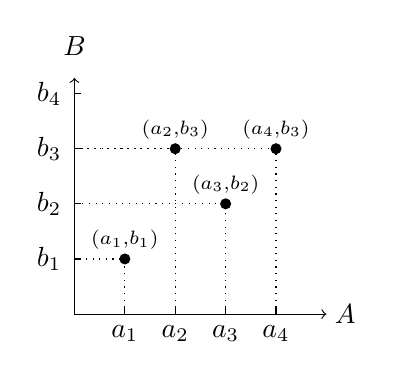
\begin{tikzpicture}[x=0.8cm]
  	\draw[->] (0,0) -- (4,0);
  	\draw[->] (0,0) -- (0,3.0);
  	\node at (4.3,0) {$A$};
  	\node at (0,3.4) {$B$};

      \draw (0.8,0) -- +(0,0.1) node [label=below:$a_1$]{};
      \draw (1.6,0) -- +(0,0.1) node [label=below:$a_2$]{};
      \draw (2.4,0) -- +(0,0.1) node [label=below:$a_3$]{};
      \draw (3.2,0) -- +(0,0.1) node [label=below:$a_4$]{};

      \draw (0,0.7) -- +(0.1,0) node [label=left:$b_1$]{};
      \draw (0,1.4) -- +(0.1,0) node [label=left:$b_2$]{};
      \draw (0,2.1) -- +(0.1,0) node [label=left:$b_3$]{};
      \draw (0,2.8) -- +(0.1,0) node [label=left:$b_4$]{};

  	\draw[dotted] (0.8,0) -- (0.8,0.7) -- (0,0.7);
  	\draw[dotted] (1.6,0) -- (1.6,2.1) -- (0,2.1);
  	\draw[dotted] (2.4,0) -- (2.4,1.4) -- (0,1.4);
  	\draw[dotted] (3.2,0) -- (3.2,2.1) -- (0,2.1);

  	\fill (0.8,0.7) circle (2pt) node[above] {$\scriptstyle (a_1,b_1)$};
  	\fill (1.6,2.1) circle (2pt) node[above] {$\scriptstyle (a_2,b_3)$};
  	\fill (2.4,1.4) circle (2pt) node[above] {$\scriptstyle (a_3,b_2)$};
  	\fill (3.2,2.1) circle (2pt) node[above] {$\scriptstyle (a_4,b_3)$};
  \end{tikzpicture}
%
\hfill
%
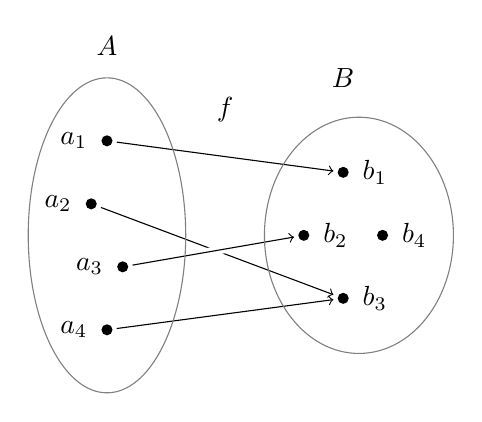
\begin{tikzpicture}[x=1cm,y=0.8cm]
\fill (1,4) circle (2pt) node (a1) [label=left:$a_1$]{};
\fill (0.8,3) circle (2pt) node (a2) [label=left:$a_2$]{};
\fill (1.2,2) circle (2pt) node (a3) [label=left:$a_3$]{};
\fill (1,1) circle (2pt) node (a4) [label=left:$a_4$]{};
\fill (4,3.5) circle (2pt) node (b1) [label=right:$b_1$] {};
\fill (3.5,2.5) circle (2pt) node (b2) [label=right:$b_2$] {};
\fill (4,1.5) circle (2pt) node (b3) [label=right:$b_3$] {};
\fill (4.5,2.5) circle (2pt) node (b4) [label=right:$b_4$] {};
\draw[->] (a1) edge (b1);
\draw[->] (a2) edge (b3);
\draw[line width=3pt,white] (a3) edge (b2);
\draw[->] (a3) edge (b2);
\draw[->] (a4) edge (b3);
\draw[draw=gray](1,2.5) ellipse (1cm and 2cm);
\draw[draw=gray](4.2,2.5) ellipse (1.2cm and 1.5cm);
\node at (1,5.5) {$A$};
\node at (4,5) {$B$};
\node at (2.5,4.5) {$f$};
\end{tikzpicture}
\hfill
\mbox{}
\caption[]{La funzione $f\colon A\to B$,
$f=\{a_1\mapsto b_1,$ $a_2 \mapsto b_3,$ $a_3 \mapsto b_2,$ $a_4 \mapsto b_3\}$
definita sull'insieme $A=\ENCLOSE{a_1, a_2, a_3, a_4}$
a valori nell'insieme $B=\ENCLOSE{b_1, b_2, b_3, b_4}$
rappresentata tramite grafico e
tramite diagrammi di Venn.}
\label{fig:funzione}
\end{figure}


L'insieme di partenza $A$ viene chiamato \emph{dominio}%
\mymargin{dominio}%
\index{dominio} 
della funzione $f\colon A\to B$,
mentre l'insieme di arrivo $B$ viene chiamato \emph{codominio}%
\mymargin{codominio}%
\index{codominio}.
La funzione $f$ rappresenta quindi un modo di assegnare in maniera univoca
ad ogni elemento del dominio un elemento del codominio.
Da un punto di vista informatico potremmo dire che $A$ è l'insieme
dei possibili \emph{input} e $B$ è l'insieme dei possibili \emph{output}
della funzione $f$.

Per come l'abbiamo definita, una funzione è dunque un insieme.
In generale le funzioni potrebbero essere definite in altri modi oppure 
potrebbero essere un concetto primitivo: dunque nei capitoli seguenti useremo le funzioni 
senza assumere che esse siano a loro volta degli insiemi.
Ad esempio invece di scrivere $(a,b)\in f$ scriveremo sempre $f(a)=b$ 
oppure $a\stackrel f \mapsto b$.
Sarà comunque molto importante
considerare l'insieme che rappresenta $f$ ma questo verrà chiamato
\emph{grafico}%
\mymargin{grafico}%
\index{grafico} di $f$, $G_f$ e potrà essere definito in questo modo:
\[
  G_f = \ENCLOSE{(x,y)\in A \times B\colon f(x)=y}.
\]
Nella nostra costruzione risulta effettivamente $G_f = f$ ma, come abbiamo detto,
in generale è opportuno distinguere la funzione dal suo grafico.
Uno degli argomenti principali di questo corso è lo studio 
del grafico delle funzioni reali, cioè le funzioni 
con dominio e codominio nell'insieme dei numeri reali.

\subsection{invertibilità}

Capita molto spesso che un fenomeno possa essere modellizzato matematicamente
tramite una funzione: si sa che ad un certo \emph{input} $a$ corrisponde
un \emph{output} $b=f(a)$. Molto spesso il problema da risolvere è
quello di determinare l'\emph{input} giusto $a$ per ottenere l'\emph{output}
voluto $b$. Questo problema corrisponde ad \emph{invertire} la funzione $f$:
dato $b\in B$ determinare $x\in A$ tale che $f(x) = b$.

Una funzione $f\colon A \to B$ si dice essere \emph{surgettiva}%
\mymargin{surgettiva}%
\index{surgettiva} (o \emph{suriettiva})
se per ogni $b\in B$ esiste almeno un $x\in A$ per cui $f(x)=b$. Questo
significa che il problema dell'inversione ha almeno una soluzione, qualunque
sia $b\in B$.
Una funzione $f\colon A \to B$ si dice essere \emph{iniettiva}%
\mymargin{iniettiva}%
\index{iniettiva}
se non esistono due punti distinti $a,a' \in A$, $a\neq a'$ tali
che $f(a) = f(a')$. Questo significa che il problema dell'inversione
$f(x)=b$ ha al più una soluzione (la soluzione, se esiste, è unica).
Una funzione $f\colon A \to B$ si dice essere \emph{bigettiva}%
\mymargin{bigettiva}%
\index{bigettiva}
(o \emph{biettiva})
\index{biettiva}%
\index{bigettiva}%
\index{funzione!bigettiva}%
\index{invertibile}%
\index{funzione!invertibile}%
\index{biettiva}%
o
\emph{invertibile}%
\mymargin{invertibile}%
\index{invertibile}%
\footnote{\textbf{Attenzione:} in alcuni testi (tra cui~\cite{Giusti}) si considerano
invertibili le funzioni iniettive, anche se non surgettive.}
se è sia iniettiva che surgettiva. Questo significa
che il problema dell'inversione $f(x)=b$ ha una unica soluzione $x\in A$
qualunque sia $b\in B$. In particolare, se $f$ è invertibile, per ogni $b\in B$ esiste
un unico $a\in A$ per cui $f(a)=b$.
Se $f$ è una funzione invertibile allora la relazione inversa $g$
cioè la relazione tale che $b\stackrel g \mapsto a$ quando $a \stackrel f \mapsto b$
risulta essere una funzione $g\colon B\to A$. 
Infatti $g$ è definita su tutto $B$ in quanto $f$ è surgettiva 
e $g$ è univoca in quanto $f$ è iniettiva.
Le proprietà caratteristiche della \emph{funzione inversa}%
\mymargin{funzione inversa}%
\index{funzione!inversa} $g$ sono:
\begin{equation}\label{eq:572098}
  \forall a\in A\colon g(f(a)) = a, \qquad
  \forall b\in B\colon f(g(b)) = b.
\end{equation}
La funzione inversa $g$ viene usualmente denotata con il simbolo $f^{-1}$.

Se $f\colon A\to B$ è bigettiva diremo che $A$ 
e $B$ sono in \emph{corrispondenza biunivoca}%
\mymargin{corrispondenza biunivoca}%
\index{corrispondenza!biunivoca} tramite $f$.
In effetti $f$ è una corrispondenza \emph{univoca} da $A$ in $B$
(manda in modo univoco ogni punto di $A$ in un punto di $B$)
e $f^{-1}$ è una corrispondenza univoca da $B$ in $A$.

Introduciamo ora delle notazioni che sarà comodo utilizzare nel seguito.
Se $f\colon A \to B$ è una funzione e se $C\subset A$ definiamo
\[
  f(C) 
  = \ENCLOSE{f(a)\colon a \in C} 
  = \ENCLOSE{b\in B\colon \exists a\in C\colon b=f(a)}.
\]
L'insieme $f(C)\subset B$ si chiama \emph{immagine}%
\mymargin{insieme immagine}%
\index{immagine}
\index{immagine!insieme}%
di $C$ (tramite $f$) ed è formato
da tutti i punti che si ottengono applicando $f$ agli elementi di $C$.
L'immagine $f(A)$ dell'intero dominio $A$ si chiama immagine di $f$
e si denota a volte con il simbolo $\Im f$.
Si noti che $f$ è surgettiva se e solo se $f(A)=B$ (cioè se l'immagine coincide
col codominio).
Ad esempio la funzione definita in Figura~\ref{fig:funzione}
ha immagine $f(A) = \ENCLOSE{f(a_1),f(a_2),f(a_3),f(a_4)} 
 = \ENCLOSE{b_1, b_2, b_3}$.

Anche se $f\colon A \to B$ non fosse iniettiva,
per ogni $C\subset B$ possiamo definire
\[
  f^{-1}(C) = \ENCLOSE{a\in A\colon f(a) \in C}.
\]
L'insieme $f^{-1}(C)\subset A$ si chiama \emph{preimmagine}
o \emph{controimmagine}
\mymargin{preimmagine}%
\index{preimmagine}%
\index{preimmagine!insieme}%
\index{controimmagine!insieme}%
\index{insieme!controimmagine}%
di $C$ (tramite $f$)
ed è formato da tutti i punti di $A$ che applicando $f$ vanno in $C$.
Si noti che se $b\in B$ l'insieme $f^{-1}(\ENCLOSE{b})$ non è altro che
l'insieme delle soluzioni dell'equazione $f(x)=b$. Come abbiamo
già visto tale insieme contiene almeno un elemento se $f$ è suriettiva,
contiene al più un elemento se $f$ è iniettiva e contiene esattamente
un elemento $f^{-1}(\ENCLOSE{b}) = \ENCLOSE{f^{-1}(b)}$ se $f$ è bigettiva.
Ad esempio se $f$ è la funzione definita in figura~\ref{fig:funzione}
si ha $f^{-1}(\ENCLOSE{b_3,b_4}) = f^{-1}(\ENCLOSE{b_3}) = \ENCLOSE{a_2,a_3}$,
$f^{-1}(\ENCLOSE{b_4}) = \emptyset$.


La notazione $f(C)$ appena introdotta è formalmente ambigua in quanto
potrebbe non essere chiaro se $C$ è un elemento oppure un sottoinsieme
del dominio di $f$.
In pratica il contesto dovrebbe rendere chiaro cosa si intende.

Più in generale ci capiterà di estendere questo abuso di notazione non solo
alle funzioni, ma anche alle relazioni e alle operazioni.
Ad esempio se $A$ e $B$ sono insiemi di numeri ci capiterà di scrivere $A\le B$
per intendere che ogni elemento di $A$ è minore o uguale ad ogni elemento di $B$
oppure $A+B$ per intendere l'insieme di tutti i numeri che si ottengono sommando
un numero di $A$ ad un numero di $B$.

\begin{exercise}
  Sia $f\colon A \to B$ una funzione qualunque. 
  Si verifichi che se $C\subset A$ e $D\subset B$ si ha 
  \[
    f^{-1}(f(C))\supset C,
    \qquad 
    f(f^{-1}(D)) \subset D. 
  \]
  
  Che ipotesi possiamo fare su $f$ per avere l'uguaglianza
  $f(f^{-1}(C)) = C$?
  E per avere $f^{-1}(f(D)) = D$?
\end{exercise}

\subsection{funzione composta}
\index{composizione!di funzioni}%

Se $f\colon A\to B$ e $g\colon B\to C$ allora un punto $a\in A$ 
viene mandato tramite $f$ in un punto $b\in B$ e 
a sua volta il punto $b$ viene mandato da $g$ in un punto 
$c \in C$. 
La funzione che manda $a$ in $c$ viene chiamata 
\emph{funzione composta}%
\mymargin{funzione composta}%
\index{funzione!composta} se denota con $g\circ f$ 
e si può definire così:
\[
g\circ f \colon A \to C, \qquad 
(g\circ f)(x) = g(f(x)).  
\]

Se abbiamo tre funzioni 
$f\colon A\to B$, $g\colon B\to C$ e $h\colon C\to D$ 
allora è facile verificare che:
\[
   h \circ (g\circ f) = (h\circ g) \circ f
\]
in quanto per ogni $x\in A$ si ha
\[
(h \circ (g\circ f)) (x) =
h(g(f(x))) = (h\circ g)(f(x)) = ((h\circ g) \circ f) (x).  
\]
Significa che l'operatore di composizione $\circ$
soddisfa la proprietà associativa.

Se $f\colon A\to B$ è bigettiva allora 
per ogni $x\in A$ e per ogni $y\in B$ si ha,
grazie a~\eqref{eq:572098},
\[
  f^{-1} (f(x)) = x,
  \qquad f(f^{-1}(y)) = y.
\]
Significa che 
\[
  f^{-1}\circ f = \id_A, 
  \qquad
  f\circ f^{-1} = \id_B
\] 
dove $\id_X\colon X\to X$
è la funzione 
\emph{identità}%
\mymargin{identità}%
\index{identità} 
\index{funzione!identità}%
cioè la funzione 
che lascia fisso ogni punto di $X$:
\mymargin{$\id_X$}%
\index{$\id$}%
\[
\id_X(x) = x \qquad \text{per ogni $x\in X$}.
\]

\begin{theorem}
Se $f\colon A\to B$ e $g\colon B\to C$ sono entrambe invertibili
anche $g\circ f\colon A\to C$ è invertibile e si ha 
\begin{equation}\label{eq:inversa_composta}
  (g\circ f)^{-1} = f^{-1}\circ g^{-1}.
\end{equation}
\end{theorem}
\begin{proof}    
Per ogni $c\in C$ esiste un unico $b\in B$ tale che $g(b)=c$ 
ed un unico $a\in A$ tale che $f(a)=b$. 
Tale $a$ è l'unico punto per cui $g(f(a))=c$ e questo dimostra che 
$g\circ f$ è bigettiva. Inoltre $x=f^{-1}(b)$ e $b=g^{-1}(c)$ 
dunque $(g\circ f)^{-1}(c) = a = f^{-1}(g^{-1}(c))$ da cui si ottiene 
\eqref{eq:inversa_composta}.
\end{proof}

\begin{exercise}
  Si verifichi che la composizione di funzioni iniettive è iniettiva e la composizione 
  di funzione suriettive è suriettiva.
\end{exercise}

\begin{definition}[restrizione]
  Se $f\colon A\to B$ è una funzione e $C\subset A$, possiamo 
  \emph{restringere} il dominio di $f$ all'insieme $C$.
  Si ottiene una nuova funzione $f\llcorner C$ che coincide con $f$
  ma che è definita solo su $C$: $f\llcorner C\colon C\to B$.
\end{definition}


\section{cardinalità}

\begin{definition}[cardinalità]
  Diremo che due insiemi $A$ e $B$ hanno la stessa \emph{cardinalità}%
\mymargin{cardinalità}%
\index{cardinalità} 
  (oppure sono \emph{equipotenti}) 
  \index{equipotenza}%
  \index{insiemi!equipotenti}%
  \index{insieme!equipotente}%
  se esiste una funzione bigettiva $f\colon A \to B$.
  Scriveremo in tal caso:
  \[
    \# A = \# B.  
  \] 
  Se esiste una funzione iniettiva $f\colon A\to B$ significa che 
  $A$ ha la stessa cardinalità di un sottoinsieme di $B$ (in quanto $f\colon A \to f(A)$
  risulta essere bigettiva). Scriveremo in tal caso:
  \[
    \# A \le \#B.
  \]
\end{definition}

Intuitivamente se due insiemi hanno la stessa cardinalità 
significa che hanno lo stesso numero di elementi.
Ma la precedente definizione riesce a catturare tale concetto senza dover 
ricorrere al concetto di numero. 
Questo ha il vantaggio di rendere questa definizione applicabile 
a qualunque insieme, anche con \emph{infiniti} elementi.

Si osservi che non abbiamo dato una definizione di $\#A$ e quindi non stiamo 
definendo cos'è la cardinalità di un insieme ma stiamo soltanto definendo 
una relazione tra insiemi che 
denotiamo, impropriamente, utilizzando una uguaglianza: $\#A = \#B$.
E' ovvio che $\#A = \#A$ in quanto l'identità $\id_A$ è bigettiva.
E' anche chiaro che se $\#A = \#B$ e $\#B = \#C$ allora $\#A = \#C$ in quanto 
componendo tra loro due funzioni bigettive si ottiene ancora una funzione 
bigettiva. 
Infine se $\#A = \#B$ allora $\#A \le \#B$ (in quanto le funzioni bigettive 
sono iniettive) ed è chiaro che se $\#A \le \#B$ e $\#B \le \#C$ allora 
$\#A\le \#C$ (in quanto composizione di funzioni iniettive è iniettiva)

Si potrebbe anche definire $\#A \ge \#B$ quando esiste $f\colon A \to B$
surgettiva. Vorremmo verificare se questo coincide con $\#B \le \#A$, 
cioè vogliamo avere il seguente.
%
\begin{theorem}\label{th:95444}
  Esiste $f\colon A\to B$ surgettiva 
  se e solo se esiste $g\colon B\to A$ iniettiva.
\end{theorem}
% 
\begin{proof}
Da un lato se esiste $g\colon B\to A$ iniettiva, allora $g$ è una bigezione 
tra $B$ e $f(B)$. La funzione inversa $f\colon f(B) \to B$ 
\footnote{Questa funzione $f$ si chiama 
\emph{inversa sinistra}
\index{inversa!sinistra}%
di $g$ in quanto si ha $f(g(y))=y$ per ogni $y\in B$}
può essere estesa a tutto $A$ fissando un valore qualunque 
(questo si può fare se $B$ non è vuoto) nei punti di $A\setminus g(B)$.
ottenendo quindi una funzione surgettiva da $A$ in $B$.
D'altro lato se esiste una funzione $f\colon A\to B$ surgettiva,
per ogni $b\in B$ l'insieme $f^{-1}(\ENCLOSE{b})$ non è mai 
vuoto e quindi è chiaro che debba esistere 
una funzione $g\colon B\to A$ tale che $g(b)$ è un qualunque elemento 
di tale insieme
\footnote{Questa funzione $g$ si chiama 
\emph{inversa destra} 
\index{inversa!destra}%
di $f$ 
in quanto $f(g(y))=y$ per ogni $y\in B$}
(qui si utilizza l'assioma~\ref{axiom:AC} discusso più sotto). 
Chiaramente $g$ è iniettiva.
\end{proof}

Nella dimostrazione del teorema precedente abbiamo utilizzato il seguente assioma 
della teoria degli insiemi che, sorprendentemente, non è conseguenza degli assiomi 
che abbiamo già introdotto finora.

\begin{axiom}[della scelta]%
  \label{axiom:AC}%
  \index{assioma!della scelta}%
  \index{scelta!assioma della}%
  \index{AC}%
  Sia $F\colon A \to \mathcal P(B)$
  una funzione tale che $F(a)\neq \emptyset$ 
  per ogni $a\in A$. Allora esiste una funzione
  $f\colon A \to B$ tale che $f(a)\in F(a)$
  per ogni $a\in A$.
\end{axiom}

L'assioma della scelta (denotato spesso con \emph{$AC$}%
\mymargin{$AC$}%
\index{AC}, \emph{axiom of choice})
è un assioma per certi versi controverso
e alcuni matematici preferiscono non utilizzarlo nelle loro dimostrazioni.
Il sistema formale che definisce la teoria degli insiemi senza 
introdurre l'assioma della scelta 
si chiama \emph{$ZF$}%
\mymargin{$ZF$}%
\index{ZF} (Zermelo-Fraenkel) mentre 
se si aggiunge l'assioma della scelta (choice) la teoria si chiama 
\emph{$ZFC$}%
\mymargin{$ZFC$}%
\index{ZFC}.

Il seguente teorema dimostra la proprietà antisimmetrica 
della relazione tra cardinalità. 
E' probabilmente il primo vero teorema (con dimostrazione decisamente non banale) 
che andiamo a dimostrare.

\begin{theorem}[Cantor-Bernstein]%
  \label{th:cantor_bernstein}%
  \index{teorema!di Cantor-Bernstein}%
  \index{Cantor-Bernstein!teorema di}%
  Se $\#A \le \#B$ e $\#B \le \#A$ allora $\#A = \#B$.
\end{theorem}
%
\begin{figure}
  \centering
  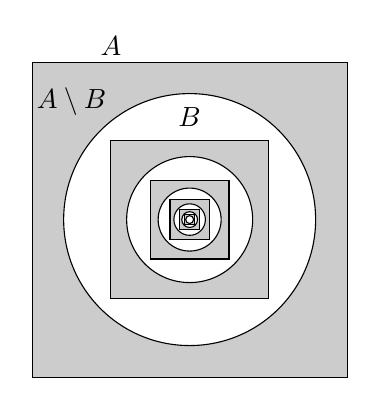
\begin{tikzpicture}
    \foreach \x in {1,0.5,0.25,0.25*0.5,0.25*0.25,0.25*0.25*0.5} {
      \path[draw,fill=black!20] (2*\x,2*\x)--(-2*\x,2*\x)--(-2*\x,-2*\x)--(2*\x,-2*\x)--cycle;
      \draw[fill=white] (0,0) circle (1.6*\x);
    };
    \node at (-1.0,2.2) {$A$};
    \node at (-1.5,1.5) {$A\setminus B$};
    \node at (0,1.3) {$B$};
%    \node at (-0.75,0.75) {$$};
  \end{tikzpicture}
  \caption{
  Nella dimostrazione del teorema di Cantor-Bernstein
  $A$ è rappresentato da un quadrato e $B$ da un cerchio contenuto
  in $A$. L'immagine di $A$ in $B$ è rappresentata da un quadrato contenuto
  in $B$ e così via. La parte ombreggiata è l'insieme $D$.
  }
  \label{fig:omotetia}
\end{figure}
%
\begin{proof}
Per ipotesi sappiamo che esiste
$g\colon B\to A$ iniettiva. 
Posto $B'=g(B)$ risulta che $g\colon B\to B'$ è bigettiva.
Ma allora dimostrare che esiste una bigezione tra $A$ e $B$ 
è equivalente a dimostrare che esiste una bigezione tra 
$A$ e $B'$. 
Dunque senza perdere di generalità, sostituendo $B'$ a $B$ 
possiamo supporre che sia $B\subset A$.

Essendo per ipotesi $\#A \le \#B$ esiste $f\colon A \to B$ iniettiva.
Intuitivamente l'idea è quella di definire l'insieme
\[
 D = (A\setminus B)  
 \cup f(A\setminus B) 
 \cup f(f(A\setminus B)) 
 \cup \dots
\]
e di definire la bigezione $\phi \colon A \to B$ 
utilizzando $f$ sull'insieme $D$ e lasciando fisso
il resto.

Per farlo in maniera rigorosa
consideriamo la famiglia di insiemi 
$\F = \{X \subset A \colon X \supset A \setminus B, f(X) \subset X\}$ 
e definiamo $D = \bigcap \F$.
Osserviamo che $A \in \F$ quindi $\F\neq \emptyset$.
Abbiamo in pratica definito $D$ come il più piccolo 
sottoinsieme di $A$ che viene mandato in se stesso da $f$.

E' facile verificare che $f(D) \subset D$ infatti dato $x\in D$ per ogni $X\in \F$ deve essere $x\in X$ ma allora $f(x) \in X$ (per come è definito $\F$), dunque $f(x) \in D$. 
In modo analogo si dimostra che $D\supset A\setminus B$ e dunque concludiamo che $D\in \F$.

Verifichiamo ora che $f(D)=D\cap B$. Da un lato se $x\in D$ allora
$f(x) \in f(D)\subset D$ e $f(x)\subset f(A)\subset B$ da cui $f(x) \in D\cap B$.
Dall'altro lato se $y\in D \cap B$ e non fosse $y \in f(D)$
allora potremmo considerare l'insieme $X=D\setminus\{y\}$
e osservare che $X\in \F$.
Infatti in primo luogo $X \supset A \setminus B$ in quanto $D$ ha questa proprietà e $y \in B$.
Inoltre dato qualunque $x \in X$ visto che $X\subset D$ allora
$f(x) \in f(D)$ e, per ipotesi,
$y\not \in f(D)$ dunque $f(x)\neq y$ da cui $f(x) \in X$.
Dunque $X\in \F$ ma allora dovrebbe essere $D\subset X$ mentre
per costruzione abbiamo $y\in D$ ma non in $X$.

% Avendo visto che $f(D)=D\cap B$ possiamo facilmente
% osservare che $f(A\setminus D) \subset A \setminus D$.
% Infatti $f(A\setminus D)\subset f(A)=B$ e quindi
% $f(A\setminus D)\cap D \subset D \cap B = f(D)$
% ma essendo $f$ iniettiva si deve avere
% $f(A\setminus D) \cap f(D)=\emptyset$.

Possiamo allora definire $\phi \colon A \to B$
\[
\phi(x) =
\begin{cases}
   f(x) & \text{se $x\in D$}, \\
   x & \text{altrimenti.}
\end{cases}
\]
Chiaramente $\phi$ è iniettiva in quanto $f$ è iniettiva e manda $D$ in $D$
e l'identità è iniettiva e manda $A\setminus D$ in $A\setminus D$.

Per dimostrare che $\phi$ è suriettiva consideriamo qualunque $y \in B$.
Se $y\not \in D$ allora $\phi(y)=y$.
Se invece $y\in D$ essendo $y\in D\cap B = f(D)$ esisterà $x\in D$ tale
che $\phi(x) = f(x) = y$.
\end{proof}

Possiamo ora determinare se un insieme $X$ è finito o infinito.
Se $f\colon X \to X$ è una funzione iniettiva allora 
$\#X = \#f(X)$.
L'idea è che togliendo anche solo un punto da un insieme finito si ottiene 
un insieme con cardinalità inferiore dunque 
non esiste una funzione iniettiva $f\colon X\to X$ che non 
sia anche suriettiva.

\begin{definition}[infinito]
  \label{def:infinito}%
  Diremo che un insieme $X$ è \emph{finito}
  \index{insieme!finito}%
  \index{finito!insieme}%
  \index{Dedekind!finito}%
  (più precisamente: Dedekind-finito)
  se ogni funzione iniettiva $f\colon X\to X$ è bigettiva.
  \mymargin{insieme finito}%
\index{insieme finito}%

  Diremo che un insieme $X$ è \emph{infinito} 
  (più precisamente Dedekind-infinito)
  \index{insieme!infinito}%
  \index{infinito!insieme}%
  \index{Dedekind!infinito}%
  se non è finito ovvero
  se esiste $f\colon X\to X$ iniettiva ma non suriettiva.
  \mymargin{insieme infinito}%
\index{insieme infinito}%
\end{definition}

Con gli assiomi che abbiamo introdotto finora non è possibile dimostrare 
che esistono insiemi infiniti. 
Ma tutti gli insiemi numerici che andremo a considerare devono essere 
insiemi infiniti... dobbiamo quindi assumere anche il seguente. 

\begin{axiom}[infinito]
  \label{axiom:infinito}%
  Esiste un insieme infinito. 
\end{axiom}

\section{i numeri naturali}

I numeri naturali $0,1,2,\dots$ sono i numeri che utilizziamo per contare o per 
fare le iterazioni. C'è un primo numero naturale, che per noi sarà $0$ e poi
per ogni numero naturale $n$ ce n'é uno successivo che chiameremo $\sigma(n)$. 
Partendo da $0$ e passando al successivo si raggiungono tutti i numeri naturali.
Queste proprietà si formalizzano come segue. 

\begin{definition}[assiomi di Peano]%
  \footnote{Giuseppe Peano (1858--1932) vedi note storiche a pag.~\pageref{note:Peano}} 
    \label{def:naturali}%
  \index{numeri!naturali}%
  \index{$\NN$}%
  \index{Peano}%
  \index{assiomi!di Peano}%
  \index{insieme!induttivo}%
  \index{induttivo}%
  Un insieme $\NN$ dotato di una 
  funzione $\sigma\colon\NN\to\NN$ e di un elemento $0\in \NN$ 
  si dice essere un insieme di 
  \emph{numeri naturali}%
\mymargin{numeri naturali}%
\index{numeri!naturali} se valgono le seguenti proprietà:
  \footnote{La proprietà 1 ci dice che $\sigma$ è iniettiva,
  la 2 che $\sigma$ non è surgettiva. 
  La 3 potrebbe essere chiamata \emph{proprietà induttiva} 
  in quanto vedremo che garantisce la validità del principio di induzione.}
  \begin{enumerate}
  \item se $\sigma(m) =\sigma(n)$ allora $m=n$;
  \item per ogni $n\in \NN$ si ha $\sigma(n)\neq 0$;
  \item se $A\subset \NN$ è un sottoinsieme tale che 
  \begin{enumerate}
    \item[i)] $0\in A$;
    \item[ii)] $n\in A \implies \sigma(n)\in A$
  \end{enumerate}
  allora $A=\NN$.
\end{enumerate}
\end{definition}

Il simbolo $\NN$ è riservato agli insiemi che soddisfano la precedente definizione.
Vedremo nel teorema~\ref{th:unicitaN} che tali insiemi 
sono tra loro indistinguibili e quindi potremo dire 
``$\NN$ è \emph{l}'insieme dei numeri naturali''
piuttosto che ``$\NN$ è \emph{un} insieme di numeri naturali''.
Ad esempio se $\NN$ è un insieme di numeri naturali 
anche $\NN_* = \NN\setminus\{0\}$
lo è scegliendo però $1\in \NN_*$ al posto di $0\in \NN$.

Dato $n\in \NN$ il numero $\sigma(n)$ si chiama il \emph{successore}%
\mymargin{successore}%
\index{successore} di $n$.
Il numero $0\in \NN$ che per assioma non è il successore di nessun'altro 
numero naturale si chiama \emph{zero}%
\mymargin{zero}%
\index{zero}. 
Per comodità diamo un nome alle \emph{cifre decimali}%
\mymargin{cifre decimali}%
\index{cifre!decimali} 
ovvero ai primi numeri naturali:
\begin{equation}\label{eq:cifre}
\begin{gathered}
 1 = \sigma(0),\quad  
 2 = \sigma(1),\quad
 3 = \sigma(2),\quad 
 4 = \sigma(3),\quad
 5 = \sigma(4),\\ 
 6 = \sigma(5),\quad 
 7 = \sigma(6),\quad 
 8 = \sigma(7),\quad 
 9 = \sigma(8)
\end{gathered}
\end{equation}
 cosicché intuiamo come la funzione $\sigma$ rappresenti 
 l'usuale operazione del contare:
 \[
 0 \stackrel\sigma\mapsto 1 \stackrel\sigma\mapsto 2 \stackrel\sigma\mapsto 
 3 \stackrel\sigma\mapsto 4 \stackrel\sigma\mapsto 5 \stackrel\sigma\mapsto 
 6 \stackrel\sigma\mapsto \dots  
 \]
Il primi due assiomi servono a garantire che in questo processo del \emph{contare}%
\mymargin{contare}%
\index{contare}
troviamo sempre numeri diversi (non si torna mai indietro) in quanto nessun numero 
può avere come successore $0$ o un numero già incontrato in precedenza (che 
se non è zero è il successore di un altro numero).

L'ultimo assioma serve a garantire che questo processo del contare esaurisca tutti 
i numeri naturali, e che quindi non ci siano dei naturali \emph{irraggiungibili}
partendo da zero.

Il fatto che $\sigma\colon \NN\to \NN$ sia iniettiva ma non suriettiva 
significa che $\NN$ può essere messo in corrispondenza biunivoca con 
$\sigma(\NN)$ che è un sottoinsieme proprio di $\NN$.
Significa che $\NN$ è un insieme infinito (definizione~\ref{def:infinito}).
In particolare $\#\NN = \#\enclose{\NN \setminus\ENCLOSE{0}}$.
Questa proprietà è per certi versi paradossale
(paradosso di Galileo)
\index{paradosso!di Galileo}%
\index{paradosso!degli insiemi infiniti}%
e caratterizza gli 
insiemi infiniti, nel senso di Dedekind.%
\footnote{Galileo Galilei (1564--1642) vedi note storiche a pag.~\pageref{nota:Galileo}}%

Normalmente la proprietà induttiva dei numeri naturali viene utilizzata tramite 
il seguente \emph{meta}-teorema.
\footnote{%
Il principio di induzione non è un teorema della teoria degli insiemi 
in quanto si riferisce il concetto di \emph{predicato} che è esterno 
al sistema stesso.}

\begin{theorem}[principio di induzione]
  Sia $P(n)$ un predicato.
  Se 
  \begin{enumerate}
    \item vale $P(0)$
    \item $\forall n\in \NN\colon P(n)\implies P(n+1)$
  \end{enumerate} 
  allora $\forall n\in \NN\colon P(n)$.
\end{theorem}
%
\begin{proof}
  Consideriamo l'insieme $A=\{n\in \NN\colon P(n)\}$.
  Grazie alle ipotesi del teorema possiamo applicare la proprietà 
  induttiva dei numeri naturali per dedurre che $A=\NN$.
  Dunque $P(n)$ è soddisfatta per ogni $n\in\NN$.
\end{proof}

Se $X$ è un qualunque insieme infinito (definizione~\ref{def:infinito}), 
dentro $X$ possiamo costruire un insieme che soddisfa gli assiomi di Peano.
Infatti fissata $f\colon X\to X$ iniettiva ma non suriettiva 
basta scegliere $0\in X\setminus f(X)$. 
Dopodiché diciamo che un sottoinsieme $I\subset X$ è \emph{induttivo}%
\mymargin{induttivo}%
\index{induttivo}
se $0\in I$ e se $n\in I\implies f(n)\in I$. Possiamo quindi definire:
\[
  \NN = \bigcap_{\text{$I\subset X$ induttivo}} I
\]
e osservare che ovviamente $\NN$ stesso è un sottoinsieme induttivo di $X$.
Dunque se $n\in \NN$ si ha $f(n)\in \NN$ e quindi la 
restrizione di $f$ a $\NN$ è una funzione $\sigma\colon \NN\to\NN$ 
che è certamente iniettiva (in quanto restrizione di una funzione iniettiva)
non è suriettiva (in quanto $0$ non è nell'immagine di $f$ 
e tantomeno nell'immagine di $\sigma$) e soddisfa la proprietà induttiva 
perché se prendiamo $A\subset \NN$ tale che $0\in A$ e $n\in A \implies \sigma(n) \in A$ 
allora significa che $A$ è induttivo e quindi, per come è definito $\NN$,
deve essere $\NN\subset A$. Dunque $A=\NN$.

La costruzione precedente ci dice che l'insieme $\NN$ è il più piccolo insieme infinito
nel senso che: se $X$ è infinito allora $\# X \ge \# \NN$. 
\footnote{Questa osservazione ci dice che se $\NN$ e $\NN'$ sono due diversi insiemi di 
numeri naturali allora $\#\NN\le \#\NN'$ e $\#\NN'\le\#\NN$ per cui, 
grazie al teorema~\ref{th:cantor_bernstein}, $\# \NN = \# \NN'$.
Nel teorema~\ref{th:unicitaN} vedremo che non solo esiste una corrispondenza biunivoca 
tra $\NN$ e $\NN'$ ma che esiste una corrispondenza che preserva la struttura (cioè l'operazione 
$\sigma$). 
}


%% \begin{comment} % DOVE SI USA?
%%   \begin{lemma}
%%     Per ogni $n\in \NN$ si ha $\sigma(n)\neq n$.
%%     \end{lemma}
%%     \begin{proof}
%%       Lo si dimostra per induzione. Per $n=0$ sappiamo che $\sigma(0)\neq 0$ 
%%       in quanto zero non è successore di nessun numero naturale.
%%       Se ora supponiamo di sapere che $\sigma(n)\neq n$ sapendo che 
%%       $\sigma$ è iniettiva possiamo dedurre $\sigma(\sigma(n))\neq \sigma(n)$ 
%%       che è proprio il passo induttivo.
%%   \end{proof}    
%% \end{comment}
  
Ora che abbiamo l'insieme infinito $\NN$ si pone la questione di come sarà possibile definire
delle funzioni su tale insieme. 
Non essendo possibile elencare tutti i valori della funzione possiamo optare 
per utilizzare la proprietà induttiva: per definire $f\colon \NN \to X$ 
basterà dire quanto vale $f(0)$ e dare una regola per definire $f(n+1)$ a partire da $f(n)$.

\begin{theorem}[definizione per induzione]
  \label{th:induzione}%
  Sia $X$ un insieme, sia $\alpha\in X$ e sia $g\colon X\to X$ una funzione.
  Allora esiste una unica funzione $f\colon \NN \to X$ tale che
  \begin{equation}\label{eq:4835628}
    \begin{cases}
      f(0) = \alpha, \\
      f(\sigma(n)) = g(f(n)).
    \end{cases}
  \end{equation}
  Si avrà dunque
  \[
    f(0) = \alpha,\quad
    f(1) = g(\alpha),\quad
    f(2) = g(g(\alpha)),\quad
    f(3) = g(g(g(\alpha)))\dots
  \]
  Più in generale se abbiamo $\alpha\in X$ e una funzione $g\colon \NN \times X \to X$
  esisterà una unica funzione $f\colon \NN \to X$ tale che
  %
  \begin{equation}
    \begin{cases}
      f(0) = \alpha, \\
      f(\sigma(n)) = g(n, f(n)).
    \end{cases}
  \end{equation}
\end{theorem}
%
\begin{proof}
Dobbiamo ricordarci che le funzioni $f\colon \NN \to X$ non sono altro che relazioni 
e cioè sottoinsiemi del prodotto $\NN\times X$.
L'idea è quindi di prendere il più piccolo sottoinsieme di $\NN\times X$ 
che possa rappresentare una funzione con le proprietà richieste.
Consideriamo dunque la famiglia di insiemi:
\[
\mathcal F = \ENCLOSE{F\in \mathcal P(\NN\times X)\colon 
  (0,\alpha)\in F,\quad (n,x)\in F \Rightarrow (\sigma(n),g(x))\in F}.
\]
Chiaramente $\mathcal F$ non è vuota in quanto $\NN\times X \in \mathcal F$.
Possiamo dunque farne l'intersezione e definire un insieme $f$:
\[
  f = \bigcap_{F\in \mathcal F} F.
\]
L'insieme $f$ che abbiamo definito rappresenta una relazione tra $\NN$ e $X$.
Visto che $(0,\alpha)\in F$ per ogni $F\in \mathcal F$ dovrà essere 
$(0,\alpha)\in f$.
Inoltre se $(n,x)\in f$ allora $(n,x)\in F$ per ogni $F\in \mathcal F$ 
e quindi $(\sigma(n),g(x))\in F$ per ogni $F\in \mathcal F$
da cui $(\sigma(n),g(x))\in f$. Significa che $f\in \mathcal F$.

Vogliamo ora dimostrare che $f$ è una funzione, cioè che è univocamente definita 
su tutto $\NN$.
Per prima cosa consideriamo l'insieme su cui $f$ è definita 
e cioè $A=\ENCLOSE{n\in \NN\colon \exists x\in X\colon (n,x)\in f}$
e dimostriamo, per induzione, che $A=\NN$.
In effetti $(0,\alpha)\in f$ quindi $0\in A$. 
E se $n\in A$ sappiamo che esiste $x\in X$ tale che $(n,x)\in f$ 
e dunque, essendo $f\in \mathcal F$, anche $(\sigma(n),g(x))\in f$
da cui $\sigma(n)\in A$. 
Abbiamo dimostrato che $f$ è definita su tutto $\NN$.

Dimostriamo ora che $f$ è univoca. Consideriamo 
l'insieme su cui $f$ è univocamente definita: 
$B=\ENCLOSE{n\in \NN\colon \exists! x\in X\colon (n,x)\in f}$.
Di nuovo vogliamo dimostrare per induzione che $B=\NN$. 
Per dimostrare che $0\in B$, visto che già sappiamo che $(0,\alpha)\in f$, 
dobbiamo dimostrare che se $x\neq \alpha$ si ha $(0,x)\not\in f$.
Sia dunque $x\neq \alpha$ e consideriamo 
l'insieme $F=f\setminus\ENCLOSE{(0,x)}$.
Chiaramente $F\in \mathcal F$ in quanto $(0,\alpha)\in F$
visto che $(0,\alpha)\in f$ e $(0,\alpha)\neq (0,x)$
inoltre se $(n,y)\in F$ allora $(n,y)\in f$ 
e quindi $(\sigma(n),g(y)) \in f$.
Ma certamente $(\sigma(n),g(y))\neq (0,x)$ in quanto $\sigma(n)\neq 0$ 
dunque $(\sigma(n),g(y))\in F$.
Visto che $F\in \mathcal F$ si deve avere $f\subset F$ e dunque 
$(0,x)\not \in f$. Dunque $f$ è univocamente definita in $0$.

Dobbiamo ora mostrare che se $n\in B$ anche $\sigma(n)\in B$.
Se $n\in B$ significa che c'è un unico $x\in X$ tale che $(n,x)\in f$
e certamente anche $(\sigma(n),g(x))\in f$.
Prendiamo allora $y\neq g(x)$, vorremo dimostrare che $(\sigma(n),y)\not \in f$.
Consideriamo, similmente a prima, l'insieme $F=f\setminus\ENCLOSE{(\sigma(n),y)}$
e cerchiamo di dimostrare che $F\in \mathcal F$.
Chiaramente $(0,\alpha)\in F$ perché $(0,\alpha)\in f$ 
e non può essere $(0,\alpha)=(\sigma(n),y)$ in quanto $\sigma(n)\neq 0$.
Se ora supponiamo che sia $(m,z)\in F$ certamente sarà $(m,z)\in f$ 
e dunque $(\sigma(m),g(z))\in f$: 
dobbiamo mostrare che $(\sigma(m),g(z))\in F$. 
D'altra parte se fosse $(\sigma(m), g(z))=(\sigma(n),y)$ 
dovrebbe essere $m=n$ in quanto $\sigma$ è iniettiva. 
Ma visto che $f$ è univocamente definita su $n$ dovrà allora essere 
anche $(n,z) = (n,x)$ e quindi $g(z)=g(x) \neq y$. 
Dunque $(\sigma(m),g(z))\in F$ e $F\in \mathcal F$.
Ma allora $f\subset F$ e quindi $(\sigma(n),y)\not \in f$.
Significa che $f$ è univocamente definita anche in $\sigma(n)$.
Per induzione $B=\NN$ ed $f$ è una funzione $f\colon \NN\to X$.

Ovviamente visto che $f\in \mathcal F$ sappiamo che $f$ 
soddisfa le proprietà richieste dal teorema.

Nella seconda parte del teorema, dove $g\colon \NN\times X \to X$,
possiamo considerare l'insieme $Y=\NN\times X$ e la funzione 
$G\colon Y\to Y$ definita da $G(n,x) = (\sigma(n), g(n,x))$.
Allora applicando la prima parte possiamo trovare $F\colon \NN\to Y$
tale che $F(0) = (0,\alpha)$ e $F(\sigma(n)) = G(F(n))$.
Basterà prendere come $f(n)$ la seconda componente di $G(n)$.
\end{proof}
  
Useremo le definizioni per induzione per definire le iterazioni e le operazioni elementari 
sui numeri naturali.

%
%
\subsection{iterazione e addizione}
%
%
\index{iterazioni}%
\index{funzione!iterata}%
\index{funzione!composta}%
Data una qualunque funzione $f\colon X \to X$ di un insieme $X$ in sé, 
possiamo fare la composizione di $f$ con se stessa, e iterare il procedimento: 
\begin{align*}
  f\circ f &\colon X\to X, 
    \qquad (f\circ f)(x) = f(f(x)),\\ 
  f\circ f \circ f&\colon X\to X,
    \qquad(f\circ f \circ f) (x) = f(f(f(x))), \dots   
\end{align*}
Utilizzando i numeri naturali possiamo definire, per induzione, 
la funzione $f^n\colon X\to X$ per ogni $n\in \NN$ 
(iterata $n$-esima):
\footnote{%
La notazione $f^n$ è ambigua in quanto può rappresentare 
sia l'iterazione della funzione composta, sia l'iterazione 
dell'operazione di prodotto (ovvero la potenza $n$-esima): 
$f^2(x) = f(f(x))$ oppure $f^2(x) = f(x) \cdot f(x)$. 
Sarà il contesto a suggerire quale sia il significato
inteso con questa notazione.
}
\begin{equation}
  \label{def:iterata}%
  \begin{cases}
    f^0 =  \id_X\\
    f^{\sigma(n)} = f\circ f^n.
  \end{cases}  
\end{equation}
%
\begin{example}
Sia $X=\ENCLOSE{1,2,3}$ e $f\colon X\to X$, $f = \ENCLOSE{1\mapsto 2, 2 \mapsto 2, 3\mapsto 1}$.
Allora le iterate di $f$ sono:
\begin{align*}
  f^0 &= \ENCLOSE{1\mapsto 1, 2\mapsto 2, 3\mapsto 3} = \id_X, \\
  f^1 &= \ENCLOSE{1\mapsto 2, 2 \mapsto 2, 3\mapsto 1} = f,\\
  f^2 &= \ENCLOSE{1\mapsto 2, 2\mapsto 2, 3\mapsto 2} = f\circ f
\end{align*}
e (lo si dimostri per induzione) per ogni $n\ge 2$ si ha $f^n = f^2$.
\end{example}

%
%
%\subsection{addizione sui numeri naturali}
%

Avendo a disposizione la funzione $\sigma\colon \NN\to\NN$ 
che manda un numero naturale nel successivo, vorremmo definire 
l'addizione su $\NN$ come iterazione della funzione $\sigma$.
Intuitivamente:
\[
  n \stackrel\sigma\mapsto n+1 \stackrel\sigma\mapsto n+2 
  \stackrel\sigma\mapsto \dots \stackrel\sigma\mapsto n+k. 
\]
Possiamo quindi definire la \emph{addizione}%
\mymargin{addizione}%
\index{addizione}:
\[
  n+k = \sigma^k(n).  
\]
In generale possiamo definire un operatore binario come una funzione 
che al secondo operando associa a sua volta una funzione che al 
primo operando restituisce il risultato:
\[
  n + k = +(k)(n).
\]
Per l'addizione si ha quindi $+(k) = \sigma^k$:
la funzione che aggiunge $k$ ad un numero è l'iterata 
$k$-esima della funzione successore.

Ad esempio:
\[
  2 + 3 
  = \sigma^3(2) 
  = \sigma(\sigma(\sigma(2))) 
  = \sigma(\sigma(\sigma(\sigma(\sigma(0))))) = 5.
\]

Osserviamo che si ha $\sigma(n) = n+1$ e per induzione 
è facile dimostrare le seguenti proprietà:
\begin{gather*}
   0 + n = \sigma^n(0) = n, \\
   \sigma(n+m) = n + \sigma(m). \label{eq:476554}
\end{gather*}

\begin{theorem}
  \label{th:iterata_composta}%
  Sia $f\colon A \to A$ una qualunque funzione.
  Allora 
  \begin{equation}\label{eq:iterata_composta}
    f^{n+m} = f^m \circ f^n = f^n \circ f^m.
  \end{equation}
\end{theorem}
%
\begin{proof}
Dimostriamo la prima uguaglianza in~\eqref{eq:iterata_composta} 
per induzione su $m$.
Per $m=0$ è ovvio in quanto $n+0 = \sigma^0(n)=\id_{\NN}(n)=n$ e $f^n=\id_A$
dunque $f^{n+0} = f^n = f^0 \circ f^n$.
Il passo induttivo richiede \eqref{eq:476554},
\eqref{def:iterata} e l'ipotesi induttiva~\eqref{eq:iterata_composta}:
\[
f^{n+\sigma(m)} 
= f^{\sigma(n+m)}
= f\circ f^{n+m}
= f\circ f^m \circ f^n
= f^{\sigma(m)}\circ f.
\]

Per dimostrare la seconda uguaglianza in~\eqref{eq:iterata_composta}
dobbiamo preliminarmente dimostrare che vale 
\begin{equation}\label{eq:5ty349}
  f\circ f^n = f^n \circ f.  
\end{equation}
Lo facciamo per induzione su $n$. Se $n=0$ ambo i lati sono uguali a $f$.
Il passaggio induttivo è il seguente:
\[
  f\circ f^{\sigma(n)} = f\circ f\circ f^n = f\circ f^n \circ f 
  = f^{\sigma(n)} \circ f.
\]
\end{proof}

Possiamo allora dedurre le seguenti familiari proprietà dell'addizione.
\begin{theorem}
  L'addizione su $\NN$ soddisfa le seguenti 
  proprietà:
  \begin{enumerate}
    \item associativa: $(n+m)+k = n + (m + k)$,
    \item elemento neutro: $n+0 = 0+n = n$,
    \item commutativa: $n+m = m+n$,
    \item invariantiva: se $m+k = n+k$ allora $m=n$.
  \end{enumerate}
\end{theorem}
\begin{proof}
Per la proprietà associativa si può utilizzare
\eqref{eq:iterata_composta}
\[
n+(m+k) 
= \sigma^{m+k}(n)
= \sigma^k \sigma^m(n) 
= \sigma^k (n+m)
= (n+m) + k.
\]

Per la proprietà commutativa ricordando che $n=\sigma^n(0)$
usiamo ancora~\eqref{eq:iterata_composta}
\[
n+m 
= \sigma^m(n)
= \sigma^m (\sigma^n (0))
= \sigma^n (\sigma^m (0)) 
= \sigma^n(m) = m+n.
\]

Per l'elemento neutro abbiamo già osservato che $0+n=n$ 
si dimostra facilmente per induzione.
E ovviamente $n+0 = \sigma^0(n) = \id(n) = n$.

Per la proprietà invariantiva 
l'uguaglianza $m+k = n+k$ è equivalente a 
\begin{equation}\label{eq:49tj9843}
  \sigma^k(m) = \sigma^k(n).  
\end{equation}
Visto che $\sigma$ è iniettiva anche $\sigma^k$ è iniettiva 
(in quanto composizione di funzioni iniettive)
dunque se vale~\eqref{eq:49tj9843} 
deve essere $m=n$, come volevamo dimostrare.
\end{proof}

% \begin{exercise}
%   Dimostrare, utilizzando il principio di induzione e le proprietà 
%   dell'addizione, la seguente 
%   proposizione:
%   \[
%   \forall n\in \NN\colon \enclose{\enclose{\exists m\in \NN \colon n = m + m} 
%   \lor \enclose{\exists m\in \NN\colon n = m + m + 1}}.  
%   \]
% \end{exercise}

\subsection{moltiplicazione}

La moltiplicazione $\cdot$ su $\NN$ è intesa come somma ripetuta:
$3\cdot n = n + n + n$. 
Intuitivamente per definire $n\cdot k$ dobbiamo iterare
la funzione $+n=\sigma^n$ che somma $n$ al numero precedente:
\[
  0\stackrel{+n}\mapsto n \stackrel{+n}\mapsto n\cdot 2 
  \stackrel{+n}\mapsto \dots \stackrel{+n}\mapsto n\cdot k.
\]
Formalmente possiamo quindi dare la seguente definizione:
\[
  n\cdot k = (+n)^k(0) = (\sigma^n)^k(0).  
\]

Chiaramente $(\sigma^n)^0=\id$ dunque $n\cdot 0=\id(0) = 0$.
Mentre $(\sigma^n)^1=\sigma^n$ dunque $n\cdot 1 = \sigma^n(0) = n$.  

Ci servirà anche osservare che risulta:
\begin{equation}\label{eq:70138875}
  n\cdot (k+1) = n\cdot k + n
\end{equation}
infatti:
\[
 n\cdot(k+1) 
 = (\sigma^n)^{k+1}(0)  
 = \sigma^n ((\sigma^n)^k(0))
 = \sigma^n (n\cdot k) = n\cdot k + n.
\]

La moltiplicazione tra naturali è legata 
alle iterazioni dai seguenti teoremi.
\begin{theorem}
  \label{th:commuta_composta}%
  Se $f,g\colon X\to X$ commutano, cioè se $f\circ g = g\circ f$ 
  allora per ogni $n\in \NN$ anche $f^n$ e $g$ commutano
  e inoltre si ha:
  \begin{equation}\label{eq:commuta_composta}
    f^n\circ g^n = (f\circ g)^n.
  \end{equation}
\end{theorem}
\begin{proof}
Possiamo dimostrare per induzione su $n$ che 
$f^m\circ f^n = f^n \circ f^m$.
Per $n=0$ ambo i lati sono uguali a $f^m$. 
Il passo induttivo utilizza~\eqref{eq:5ty349}
\[
f^m \circ f^{\sigma(n)} 
= f^m \circ f \circ f^n 
= f\circ f^m \circ f^n  
= f \circ f^n \circ f^m
= f^{\sigma(n)} \circ f^m. 
\]

Supponiamo ora che $f\circ g = g\circ f$ e dimostriamo per 
induzione che $f^n\circ g = g\circ f^n$:
\[
f^{n+1}\circ g 
= f \circ f^n \circ g 
= f \circ g \circ f^n 
= g \circ f \circ f^n
= g \circ f^{n+1}.
\]
Possiamo quindi dimostrare per induzione che $f^n\circ g^n = (f\circ g)^n$:
\[
f^{n+1}\circ g^{n+1}
=f\circ f^n \circ g \circ g^n
=f\circ g\circ f^n\circ g^n 
= (f\circ g) \circ (f\circ g)^n
= (f\circ g)^{n+1}. 
\]
\end{proof}

\begin{theorem}[iterata dell'iterata]
Sia $f\colon X\to X$ una funzione qualunque e siano $n,m\in\NN$.
Allora 
\begin{equation}\label{eq:iterazione_iterazione}
  f^{n\cdot m} = (f^n)^m = (f^m)^n.    
\end{equation}
\end{theorem}
%
\begin{proof}
Dimostriamo entrambe le uguaglianze per induzione su $m$.
Per $m=0$ tutti e tre i termini sono uguali all'identità.

Il passo induttivo per dimostrare $f^{n\cdot m}=(f^n)^m$ 
usa~\eqref{eq:70138875}:
\[
f^{n\cdot (m+1)}
=f^{n\cdot m + n } 
= f^n \circ f^{n\cdot m}
= f^n \circ (f^n)^m
= (f^n)^{m+1}.
\]

Per dimostrare $(f^n)^m = (f^m)^n$ 
il passo induttivo sfrutta~\eqref{eq:iterazione_iterazione}
e~\eqref{eq:commuta_composta}:
\[
(f^n)^{m+1}
= f^n \circ (f^n)^m
= f^n \circ (f^m)^n
= (f\circ f^m)^n
= (f^{m+1})^n.
\]
\end{proof}

\begin{theorem}[proprietà della moltiplicazione]
La moltiplicazione su $\NN$ soddisfa le seguenti proprietà:
\begin{enumerate}
  \item elemento neutro e assorbente: $n\cdot 1=n$, $n\cdot 0=0$,
  \item proprietà distributiva: $n\cdot(k+j) = n\cdot k + n\cdot j$,
  \item proprietà associativa: $n\cdot(m\cdot k) = (n\cdot m)\cdot k$,
  \item proprietà commutativa: $n\cdot m = m\cdot n$.
\end{enumerate}
\end{theorem}
\begin{proof}
Le proprietà dell'elemento neutro ed assorbente le abbiamo già 
dimostrate.

Per le altre proprietà bisogna osservare che 
$\sigma$, $\sigma^m$, $\sigma^n$, $(\sigma^n)^j$ commutano,
dunque
\[
  (\sigma^n)^j(m) 
  = (\sigma^n)^j\circ \sigma^m (0)
  = \sigma^m \circ (\sigma^n)^j (0)
  = \sigma^m(n\cdot j)
  = n\cdot j + m.
\]

Per la proprietà distributiva:
\[
n\cdot (k+j)  
= (\sigma^n)^{k+j}(0)
= (\sigma^n)^j \circ (\sigma^n)^k(0)
= \sigma^{n\cdot j}(\sigma(n\cdot k)(0))
= \sigma^{n\cdot j}(n\cdot k)
= n \cdot k + n\cdot j.
\]

Per la proprietà associativa:
\[
n\cdot (m\cdot k)
= (\sigma^n)^{m\cdot k}(0)
= ((\sigma^n)^m)^k(0)
= (\sigma^{n\cdot m})^k(0)
= (n\cdot m)\cdot k.
\]

Per la proprietà commutativa usiamo~\eqref{eq:iterazione_iterazione}
\[
  n\cdot m
  = (\sigma^n)^m(0) 
  = (\sigma^m)^n(0)
  = m\cdot n. 
\]
\end{proof}

\subsection{elevamento a potenza}

L'elevamento a potenza si definisce come un prodotto ripetuto: 
$k^3 = k\cdot k\cdot k$.
Se consideriamo la funzione $\cdot k$ 
che moltiplica un numero naturale per $k$:
\[
 \cdot k(n) = n\cdot k  
\]
Possiamo definire le potenze di $k$ in questo modo:
\[
   k^n = (\cdot k)^n(1).  
\]
Osserviamo che più in generale si ha 
\begin{equation}\label{eq:3954820}
  (\cdot k)^n(m) = m\cdot k^n
  \qquad\text{ovvero}\qquad
 (\cdot k)^n = \cdot(k^n).
\end{equation}


Si osservi che la definizione di $k^n$ è valida per ogni $n\in \NN$ e 
per ogni $k\in \NN$. 
Visto che $(\cdot k)^0 = \id$ si ha $k^0=1$ per ogni $k\in \NN$,
anche per $k=0$.
Dunque abbiamo consapevolmente definito $0^0=1$:
questa definizione (controversa) risulterà essere utile.
Si osservi che qualunque numero moltiplicato per $0$ dà zero, 
quindi una moltiplicazione ripetuta per $0$ da sempre zero se c'è almeno 
un fattore: $0^n=0$ se $n>0$. 
Ma nel prodotto $0^0$ ci sono $0$ fattori $0$ quindi non c'è nessuna 
moltiplicazione per $0$. 
E' dunque naturale che il risultato sia $1$, 
l'elemento neutro della moltiplicazione.

Usando le proprietà dell'iterazione possiamo dimostrare il seguente.
\begin{theorem}[proprietà delle potenze]
  L'elevamento a potenza definito su $\NN$ ha le seguenti proprietà
  (per ogni $k,n,m\in \NN$):
  \begin{enumerate}
    \item $k^0 = 1$,
    \item $k^{n+m} = k^n \cdot k^m$,
    \item $(k^n)^m = k^{n\cdot m}$,
    \item $(k\cdot j)^n = k^n\cdot j^n$. 
  \end{enumerate}
\end{theorem}
%
\begin{proof}
Abbiamo già discusso la prima proprietà $k^0 = (\cdot k)^0(1) = \id(1) = 1$.

Per la seconda proprietà usando~\eqref{eq:3954820},
la definizione e le proprietà dell'iterazione:
\[
(\cdot k)^{n+m}(1)
= (\cdot k)^n((\cdot k)^m(1))
= (\cdot k)^n(k^m)
= k^m \cdot k^n.
\]

Per la terza proprietà
si ha: 
\[
\cdot((k^n)^m) 
= ((\cdot k)^n)^m
= (\cdot k)^{m\cdot n}.
\]

Infine dalla commutatività della moltiplicazione 
possiamo dedurre che $\cdot k$ e $\cdot j$ commutano,
quindi, grazie a~\eqref{eq:commuta_composta}:
\[
(\cdot k\circ \cdot j)^n = (\cdot k)^n \circ (\cdot j)^n  
\]
da cui si ottiene la quarta proprietà.
\end{proof}

\subsection{ordinamento}
Possiamo ora definire una relazione $\le$ su $\NN$ ponendo 
\[
  m \le n \iff \exists k\in \NN\colon n = m+k.  
\]
Se $m\le n$ tale numero 
$k$ è unico in quanto se fosse $m+j=n=m+k$ potremmo dedurre $k=j$
dalla proprietà invariantiva della addizione. 
Possiamo dunque definire la \emph{differenza}%
\mymargin{differenza}%
\index{differenza}: $k=n-m$.

Vogliamo dimostrare che la relazione $\le$ appena introdotta 
è una relazione d'ordine, in base alla seguente.

\begin{definition}[relazione d'ordine]
  \label{def:ordine}%
  Una relazione
  $\le$ su un insieme $X$ viene detta
  \emph{relazione d'ordine}%
\mymargin{relazione d'ordine}%
\index{relazione!d'ordine}
  se soddisfa le seguenti proprietà (per ogni $x,y,z\in X$):
  \begin{enumerate}
    \item[1.] riflessiva: $x\le x$;
    \item[2.] antisimmetrica: $x\le y \land y\le x \implies x=y$;
    \item[3.] transitiva: $x\le y \land y\le z \implies x\le z$.
  \end{enumerate}
  Si dice inoltre che la relazione d'ordine $\le$
  è una relazione d'\emph{ordine totale}%
\mymargin{ordine totale}%
  (o \emph{lineare}) 
  \index{ordinamento!totale}%
  \index{ordinamento!lineare}%
  \index{totale!ordine}%
  \index{lineare!ordine}%
  e si dice che $X$ è \emph{totalmente ordinato} se vale
  \index{totalmente ordinato}%
  \begin{enumerate}
    \item[4.] dicotomia: $x\le y \lor y\le x$.
  \end{enumerate}
\end{definition}

In generale, se $\le$ è una relazione d'ordine su $X$ si definisce la 
relazione inversa $\ge$ ponendo $x\ge y$ quando $y\le x$.
La proprietà riflessiva identifica gli ordinamenti \emph{larghi}.
Si definisce il corrispondente ordinamento stretto $<$
ponendo $x < y$ quando $x\le y \land x\neq y$
e la relazione inversa $>$ ponendo $x>y$ quando $y<x$.
  
\begin{theorem}
La relazione $\le$ è una relazione d'ordine totale su $\NN$.
\end{theorem}
%
\begin{proof}
  Il fatto che $x+0=x$ dimostra la proprietà riflessiva.
  
  Per la proprietà transitiva è sufficiente osservare
  che se $y=x+k$ e $z=y+j$ allora $z=x+k+j$.

  Per la proprietà antisimmetrica supponiamo di avere $x=y+k$ 
  e $y=x+j$. Deduciamo che $x+k+j = y +k+j$ da cui $x=y$
  per la proprietà invariantiva dell'addizione.
  
  Per mostrare che l'ordinamento è totale dobbiamo invece 
  procedere con una dimostrazione per induzione. 
  Per induzione su $x\in \NN$ vogliamo mostrare 
  che per ogni $y\in \NN$ si ha $x\le y$ oppure $y\le x$. 
  Se $x=0$ il fatto è ovvio in quanto $y=y+0$ e quindi $y\ge 0$
  per ogni $y\in \NN$.
  Supponiamo ora di sapere che $x\le y$ oppure $y\le x$.
  Se $y\le x$ significa che $x = y + k$ per un qualche 
  $k\in \NN$. Ma allora $x+1 = y + k + 1$ e quindi 
  vale anche $y\le x+1$. 
  Se invece $x\le y$ significa che esiste $k\in \NN$ 
  per cui $y=x+k$. Se $k\neq 0$ allora $k=1+j$ con $j\in \NN$
  da cui $y=x+1+j$ e dunque anche $x+1\le y$.
  Se $k=0$ allora $x=y$ e dunque $x+1=y+1$ che ci porta 
  alla disuguaglianza inversa $x+1\ge y$.
  In ogni caso il passo induttivo è dimostrato.
\end{proof}

\begin{exercise}
  Dimostrare per induzione che per ogni $n\in \NN$, $n\ge 4$ si ha 
  \[  
    2^n \ge n^2.
  \]
\end{exercise}

\subsection{rappresentazione posizionale dei numeri naturali}

Per rappresentare in modo efficiente qualunque numero naturale utilizziamo la 
\emph{notazione posizionale decimale}%
\mymargin{notazione posizionale decimale}%
\index{notazione!posizionale decimale}.
Ricordiamo che le cifre decimali $0,1,2,\dots, 9$ sono state definite in~\eqref{eq:cifre}
a pag~\pageref{eq:cifre}.
Il numero rappresentato da una sequenza finita di cifre decimali può essere 
definito ricorsivamente: una sequenza di una sola cifra rappresenta il numero 
corrispondente alla cifra stessa, una sequenza di $n+1$ cifre rappresenta il 
numero rappresentato dalle prime $n$ cifre, moltiplicato per $9+1$ (cioè dieci),
e sommato alla ultima cifra. 
Ad esempio la sequenza di cifre $4701$ (leggi: quattromilasettecentouno)
è definita così:
\[ 
  4701 = ((4\cdot(9+1)+7)\cdot(9+1)+0)\cdot(9+1)+1.
\]
Osservando che $10 = 9+1$ si scriverà
\begin{align*}
  4701 
  & = ((4\cdot 10 + 7)\cdot 10 +0)\cdot 10 + 1 \\
  & = \mathbf 4\cdot 10^3 + \mathbf 7\cdot 10^2 + \mathbf 0\cdot 10^1 + \mathbf 1 \cdot 10^0. 
\end{align*}

\subsection{fattoriale e semi-fattoriale}

Definiamo il 
\emph{fattoriale}%
\mymargin{fattoriale}%
\index{fattoriale} 
\index{"!}%
\index{$n$"!}%
denotato con $n!$ (leggi: $n$ fattoriale) 
tramite la seguente definizione ricorsiva
\[
  \begin{cases}
    0! = 1 \\
    (n+1)! = (n+1) n!
  \end{cases}
\]
in tal modo risulta che $n!$ sia il prodotto dei primi $n$ numeri naturali positivi:
\[
  n! = 1 \cdot 2 \cdot 3 \cdots n.  
\]

\begin{exercise}
  \label{ex:6734098}%
  Utilizzando il principio di induzione
  si dimostri che per ogni $n\in \NN$:
  \[
    (n+1)! \ge 2^n, \qquad
    n^n \ge n!
  \]
\end{exercise}

\begin{table}
  \begin{center}
  \begin{tabular}{r|>{\small}r>{\small}r>{\small}r>{\small}r>{\small}r}
  $n$       & 0 & 1 & 2 & 3 & 4 \\
  \footnotesize $n+5$     & 5 & 6 & 7 & 8 & 9 \\ \hline
  $2^n$     & 1 & 2 & 4 & 8 & 16 \\
  \footnotesize $2^{5+n}$ & 32 & 64 & 128 & 256 & 512 \\
  \footnotesize $2^{10+n}$ & 1024 & 2048 & 4096 & 8192 & 16384 \\
  \footnotesize $2^{15+n}$ & 32768 & 65536 & 131072 & 262144 & 524288 \\
  \footnotesize $2^{20+n}$ & 1048576 & 2097152 & 4194304 & 8388608 & 16777216 \\  \hline
  $3^n$                    & 1 & 3 & 9 & 27 & 81 \\
  \footnotesize $3^{5+n}$  & 243 & 729 & 2187 & 6561 & 19683 \\  \hline
  $n!$      & 1 & 1 & 2 & 6 & 24 \\
  \footnotesize $(5+n)!$  & 120 & 720 & 5040 & 40320 & 362880 \\
  \footnotesize $(10+n)!$  & 3628800 & 39916800 & 479001600 & 6227020800 & 87178291200 \\ \hline
  \footnotesize $10^{3n}$  &  & K (chilo) & M (mega) & G (giga) & T (tera) \\ 
  \footnotesize $10^{3(n+5)}$  & P (peta) & E (exa) & Z (zetta) & Y (yotta) \\ \hline
  \footnotesize $2^{10n}$  &  & Ki (chibi) & Mi (mebi) & Gi (gibi) & Ti (tebi) \\
  \footnotesize $2^{10(n+5)}$ & Pi (pebi)& Ei (exbi) & Zi (zebi) & Yi (yobi)
  \end{tabular}
  \end{center}
  \caption{I primi valori (e nomi) di alcune delle sequenze che abbiamo definito.}
  \end{table}
  
  A volte sarà utile considerare anche i prodotti di solamente i numeri
  pari o i numeri dispari fino ad un certo numero $n$. Questo
  si chiama \emph{semi-fattoriale}%
\mymargin{semi-fattoriale}%
\index{semi-fattoriale} e si indica con $n!!$. 
  Lo possiamo definire separatamente sui numeri pari (cioè 
  i numeri che si possono scrivere nella forma $2n$ con $n\in \NN$)
  e i numeri dispari (che scriviamo nella forma $2n+1$):
  \index{"!"!}
  \index{$n$"!"!}
  \index{doppio fattoriale}%
  \index{fattoriale!doppio}%
  \index{fattoriale!semi-fattoriale}%
  \index{semi-fattoriale}%
  \begin{align*}
    (2n)!! &= 2 \cdot 4 \cdot 6 \cdots (2n) \\
    (2n+1)!! &= 1 \cdot 3 \cdot 5 \cdots (2n+1).
  \end{align*}
  
  \begin{remark}
  \label{rem:doppio_fattoriale}%
  Si osservi che risulta
  \[
    (2n)!! = (2\cdot 1) \cdot (2\cdot 2) \cdot (2\cdot 3) \cdots (2\cdot n)
          = 2^n \cdot n!
  \]
  mentre
  \[
    2^n \cdot n! \cdot (2n+1)!! 
    = (2n)!! \cdot (2n+1)!!
    = (2n+1)!
  \]
  Queste formule permettono di esprimere il semi-fattoriale utilizzando
  il fattoriale intero e le potenze.
  \end{remark}
  
\begin{exercise}
  Si dia una definizione per induzione del semi-fattoriale
  (separatamente per i pari e per i dispari)
  e si dimostrino, per induzione, le formule nell'osservazione precedente.
\end{exercise}

\subsection{buon ordinamento e unicità dei numeri naturali}

\begin{definition}[maggiorante, minorante, massimo, minimo, limitato]
  \label{def:minorante}%
  \label{def:maggiorante}%
  \label{def:minimo}%
  \label{def:limitato}%
  Sia $\le$ una relazione d'ordine su un insieme $X$ e siano 
  $a\in X$ e $A\subset X$.

  Diremo che $a$ è un \emph{minorante}%
\mymargin{minorante}%
\index{minorante} di $A$ e scriveremo:
  \[
    a \le A
  \]
  se per ogni $x\in A$ risulta $a\le x$. 
  Se esiste $a$ per cui $a\le A$ diremo che $A$ 
  è inferiormente limitato.
  Se $a$ è un minorante e inoltre $a\in A$ diremo 
  che $a$ è il \emph{minimo}%
\mymargin{minimo}%
\index{minimo} di $A$ e scriveremo:
  \[
    a = \min A.  
  \] 

  Analogamente diremo che $a$ è un \emph{maggiorante}%
\mymargin{maggiorante}%
\index{maggiorante}
  di $A$ e scriveremo $a \ge A$ se $a\ge x$ per ogni $x\in A$,
  diremo che $A$ è superiormente limitato 
  se esiste $a$ per cui $a \ge A$ infine
  diremo che $a$ è il \emph{massimo}%
\mymargin{massimo}%
\index{massimo} di $A$ 
  e scriveremo $a=\max A$ se $a\ge A$ e $a\in A$.

  Se $A$ è superiormente limitato e inferiormente limitato
  diremo che $A$ è limitato.
\end{definition}

Massimo e minimo di un insieme $A$, se esistono, sono unici.
Infatti se $x$ e $y$ fossero due minimi di $A$ si avrebbe $x\le y$ in
quanto $x\le A$ e $y\in A$. Analogamente si avrebbe $y\le x$ e
quindi $x=y$. Ragionamento analogo se $x$ e $y$ fossero due massimi.

Se $A$ è un insieme finito il massimo e il minimo 
esistono sempre. 
\footnote{
  Se $A$ non avesse minimo potrei definire per induzione 
  una funzione $f\colon \NN\to A$ tale che $f(0)\in A$ 
  è qualunque e $f(n+1) < f(n)$ (visto che $f(n)$ non è un minimo 
  di $A$ esiste un numero più piccolo). 
  Chiaramente $f$ è iniettiva quindi $\#A\ge \#\NN$
  e dunque $A$ è infinito.
}

\begin{theorem}[principio del buon ordinamento]
  \label{th:buon_ordinamento}
  Sia $A\subset \NN$, $A\neq \emptyset$. 
  Allora $A$ ha minimo.
\end{theorem}
%
\begin{proof}
  Osserviamo che se $n\in \NN$ è un minorante di $A\subset \NN$ 
  allora o $n\in A$ e quindi $n$ è il minimo di $A$
  oppure anche $n+1$ è un minorante di $A$ in quanto 
  non ci sono numeri naturali strettamente compresi tra $n$ e $n+1$.
  \footnote{Se ci fosse un numero naturale tra $n$ e $n+1$ 
  sottraendo $n$ avremmo un numero naturale tra $0$ e $1$. 
  Ma non esiste $x\in \NN$ tale che $0<x<1$.
  Infatti se $x\in \NN$, $x>0$ allora $x\neq 0$ e quindi 
  esiste $m\in \NN$ tale che $x=m+1$. 
  Ma allora $x\ge 1$.}
  Dunque se $A$ non avesse minimo, per il principio di induzione 
  ogni $n\in\NN$ sarebbe un minorante di $A$.
  In tal caso $A$ dovrebbe essere vuoto perché se esistesse $a\in A$ 
  certamente $a+1$ non sarebbe un minorante di $A$.
\end{proof}

Vogliamo ora dimostrare che l'insieme dei numeri naturali è sostanzialmente 
unico nel senso che se ci sono due insiemi che soddisfano gli assiomi di 
Peano allora è possibile mettere in corrispondenza gli elementi dei due insiemi 
in modo che lo zero vada in zero e numeri corrispondenti abbiano successori 
corrispondenti.

\begin{theorem}[unicità dei numeri naturali]
  \label{th:unicitaN}%
  Se $\NN$ e $\NN'$ sono due insiemi che soddisfano gli assiomi di Peano 
  con zero $0\in \NN$ e $0'\in \NN'$ e funzioni 
  successore $\sigma$ su $\NN$ e $\sigma'$ su $\NN'$ allora
  esiste una funzione bigettiva $f\colon \NN\to \NN'$ tale che 
  $f(0) = 0'$ e $f(\sigma(n)) = \sigma'(f(n))$.
\end{theorem}
%
\begin{proof}
Possiamo definire $f$ per induzione:
\[
\begin{cases}
  f(0) = 0' \\ 
  f(\sigma(n)) = \sigma'(f(n))
\end{cases}  
\]
così rimane solo da dimostrare che $f$ è una bigezione.

Per dimostrare che $f$ è iniettiva consideriamo l'insieme 
\[
  A=\ENCLOSE{a\in \NN\colon \exists b\in \NN\colon b\neq a, f(a)=f(b)}.
\]
Se tale insieme è vuoto allora $f$ è effettivamente iniettiva.
Supponiamo allora per assurdo che $A$ non sia vuoto.
In tal caso possiamo considerare il minimo $a=\min A$ 
(grazie al teorema~\ref{th:buon_ordinamento}).
Dovrà quindi esistere $b\in \NN$ tale che $b\neq a$ e $f(b)=f(a)$.
Ovviamente anche $b\in A$ e quindi dovrà essere $b>a$ in quanto
$a$ è il minimo. Dunque $b>0$ e $f(b) = f(\sigma(b-1))
=\sigma'(f(b-1))$. Se $a=0$ abbiamo $f(a)=0'$ e quindi da $f(a)=f(b)$ 
otteniamo che $0'$ è nell'immagine di $\sigma'$ che è contrario 
agli assiomi di Peano. 
Se invece $a>0$ si avrà, come per $b$,
$f(a)=\sigma'(f(a-1))$ e dunque $\sigma'(f(a-1)) = \sigma'(f(b-1))$.
Per l'iniettività di $\sigma'$ si deduce $f(a-1)=f(b-1)$ da cui 
$a-1 \in A$. Ma questo è assurdo in quanto $a$ era il minimo di $A$.

Per dimostrare che $f$ è surgettiva consideriamo l'immagine 
$B'=f(\NN)$ e usiamo il principio di induzione su $\NN'$ 
per dimostrare che $B'=\NN'$.
Per prima cosa $0'\in B'$ in quanto $0'=f(0)$.
Se poi $n'\in B'$ allora esiste $n\in \NN$ tale che $f(n)=n'$.
Ma allora $f(\sigma(n))=\sigma'(f(n))=\sigma'(n')$ 
e dunque anche $\sigma'(n')\in B$. 
\end{proof}

\subsection{cardinalità finite}

Vogliamo ora dimostrare che i numeri naturali possono essere utilizzati 
per contare gli elementi degli insiemi finiti.

\begin{definition}[numero di elementi]
Se $n\in \NN$ denotiamo con 
\[
  \Enclose{n} 
  = \ENCLOSE{0,1,\dots, n-1}
  = \ENCLOSE{k\in \NN\colon k<n}
\]
l'insieme dei primi $n$ numeri naturali.
\footnote{Siccome per noi il primo numero naturale è $0$, c'è uno scarto di 
una unità tra gli ordinali \emph{primo}, \emph{secondo}, \emph{terzo}\dots e i cardinali \emph{zero},
 \emph{uno}, \emph{due}\dots
La cosa può sembrare strana ma in realtà è perfettamente \emph{naturale}
e infatti in gran parte dei linguaggi di programmazione moderni quando 
si itera una operazione $n$ volte si conta da $0$ a $n-1$.}
Questo è il prototipo di insieme con $n$ elementi.
Allora informalmente andremo a identificare $\#\Enclose{n}$ con $n$ e 
dunque scriveremo 
\[
   \#A = n, \qquad \#A\ge n, \qquad \#A\le n
\]
per significare rispettivamente
\[
  \#A = \#\Enclose{n}, \qquad \#A \ge \#\Enclose{n}, \qquad \#A\le \#\Enclose{n}.  
\]

La cardinalità di $\NN$ viene a volte indicata con il simbolo
\index{$\aleph_0$}%
\index{aleph}%
$\aleph_0$ dunque potremo scrivere  
\footnote{%
Il simbolo $\aleph$ è la prima lettera dell'alfabeto ebraico 
e si legge \emph{aleph}. \\
Abbiamo già osservato che $\NN$ è il \emph{più piccolo} insieme 
infinito dunque $\aleph_0$ è la più piccola 
cardinalità infinita. 
Si potrebbe anche dimostrare che deve esistere una cardinalità $\aleph_1>\aleph_0$
che è la più piccola cardinalità maggiore di $\aleph_0$.
Sappiamo che $\# \mathcal P(\NN)>\# \NN$ ma curiosamente non è possibile dimostrare 
che $\aleph_1 = \# \mathcal P(\NN)$ (questa si chiama \emph{ipotesi del continuo}
\index{ipotesi!del continuo}%
\index{continuo!ipotesi del}%
in quanto vedremo nel teorema~\ref{th:cantor_secondo} che $\# \mathcal P(\NN)=\#\RR$
e l'insieme $\RR$ viene chiamato \emph{continuo} là dove $\NN$ 
viene chiamato \emph{discreto}).
Dunque l'ipotesi del continuo è un ulteriore assioma che potrebbe essere 
aggiunto agli assiomi della teoria degli insiemi: 
non esistono insiemi con cardinalità strettamente compresa tra 
le cardinalità di $\NN$ e di $\mathcal P(\NN)$.
}%
\[
    \# A = \aleph_0, \qquad
    \#A \le \aleph_0, \qquad
    \# A\ge \aleph_0
\]
per significare rispettivamente 
\[
  \# A = \# \NN, \qquad
  \# A \le \# \NN, \qquad
  \# A \ge \# \NN.  
\]
\end{definition}
  
\begin{lemma}\label{lm:nfinito}
Per ogni $n\in \NN$ l'insieme $[n]=\ENCLOSE{0,1,2, \dots, n-1}$ è 
finito (nel senso di Dedekind, definizione~\ref{def:infinito}).
\end{lemma}
%
\begin{proof}
Lo possiamo dimostrare per induzione su $n\in \NN$.
Per $n=0$ si ha $[n]=\emptyset$ ed è ovvio che ogni funzione 
$f\colon \emptyset \to \emptyset$ è bigettiva. 
Dunque $[0]=\emptyset$ è finito.

Supponiamo allora che $[n]$ sia finito e supponiamo per assurdo che $[n+1]$ sia 
infinito.
Allora esiste $f\colon [n+1]\to[n+1]$ iniettiva ma non surgettiva. 
Se componiamo $f$ con la funzione $s$ che scambia $n$ con $f(n)$ otteniamo 
una funzione $g = s\circ f$ tale che $g(n)=n$.
Se $f$ era iniettiva ma non surgettiva anche $g$ mantiene le due proprietà.
Inoltre $g$ può essere ristretta a $[n]$ (in quanto $g(k)=n$ solo per $k=n$ 
visto che $g$ è iniettiva): $g\colon [n]\to [n]$
e anche la funzione ristretta risulterebbe essere iniettiva e suriettiva.
Ma questo è assurdo perché per ipotesi induttiva $[n]$ è finito.
\end{proof}

\begin{theorem}[caratterizzazione insiemi finiti]
Un insieme $A$ è infinito (nel senso di Dedekind, definizione~\ref{def:infinito})
se e solo se $\# A \ge \aleph_0$.
Viceversa $A$ è finito se e solo se esiste $n\in\NN$ tale che $\# A = n$.
\end{theorem}
%
\begin{proof}
Se $\#A \ge \aleph_0$ significa che esiste una funzione 
iniettiva $f\colon \NN\to A$. 
Dunque se definiamo $\sigma \colon A \to A$ come
\[
\sigma(a) = \begin{cases}
  a & \text{se $a\not\in f(\NN)$}\\
  f(n+1) & \text{se $a=f(n)$ con $n\in\NN$}
\end{cases}
\]
otteniamo una funzione iniettiva ma non suriettiva 
(in quanto $\sigma(A) = A\setminus\ENCLOSE{f(0)}$).
Dunque se $\#A\ge \aleph_0$ deduciamo che $A$ è infinito

Viceversa se $A$ è infinito significa che esiste $\sigma\colon A \to A$ 
iniettiva ma non suriettiva. 
Preso $\alpha \in A \setminus\sigma(A)$
possiamo definire induttivamente $f\colon \NN\to A$ come segue:
\[
\begin{cases}
  f(0) = \alpha\\
  f(n+1) = \sigma(f(n))
\end{cases}
\]
e possiamo verificare che $f$ è iniettiva. 
Infatti supponiamo che sia $f(n)=f(m)$.
Se $f(n)=f(m)=\alpha$ allora necessariamente $n=m=0$ 
perché $f(n)=\alpha$ è equivalente a $n=0$ visto che $\sigma$
non assume mai il valore $\alpha$.
Se $f(n)=f(m)\neq \alpha$ significa dunque che $n>0$ e $m>0$
ma allora $f(n)=\sigma(f(n-1))$ e $f(m)=\sigma(f(m-1))$
e dunque, essendo $\sigma$ iniettiva, $n-1=m-1$ da cui $n=m$. 
Dunque se $A$ è infinito si ha $\#\NN\le \#A$
(in realtà l'avevamo già osservato: $\NN$ è il più piccolo insieme infinito).

Dobbiamo ora caratterizzare gli insiemi finiti.
Abbiamo già verificato che se $\#A \ge \aleph_0$ 
allora $\#A$ è infinito, dunque se $\#A$ è finito 
non può essere $\#A \ge \aleph_0$.
Ma da questo non possiamo immediatamente 
dedurre che $\#A < \aleph_0$ (vedi nota a margine).%
\footnote{%
Per dimostrare che ogni cardinalità può essere confrontata 
con ogni altra (cioè che l'ordinamento dato dalla cardinalità è totale) 
bisogna dimostrare che ogni insieme ammette un buon 
ordinamento. La cosa diventa molto tecnica e richiede,
l'utilizzo dell'assioma della scelta.
}%

Se $\#A = n$ significa che $\#A = \#\Enclose{n}$ e 
grazie al lemma~\ref{lm:nfinito} sappiamo che $[n]$ è finito 
e dunque anche $A$ è finito.

Supponiamo ora che $A$ sia un insieme per il quale per ogni $n\in \NN$ 
si ha $\#A > n$. Dobbiamo dimostrare che $A$ è infinito.
Per ogni $n\in \NN$ scegliamo
una funzione iniettiva $f_n\colon\Enclose{n}\to A$.
\footnote{Qui stiamo usando l'assioma della scelta}%
Dalle $f_n$ possiamo definire le funzioni iniettive $g_n\colon \Enclose{n}\to A$
in modo che $g_{n+1}$ sia una estensione di $g_n$.
Basterà infatti porre:
\[
  \begin{cases}
  g_0 = f_0,\\
  g_{n+1}(k) = \begin{cases}
    g_n(k) &\text{se $k<n$}\\
    \min f_{n+1}([n+1])\setminus g_n([n]) & \text{altrimenti}
    \end{cases}
  \end{cases}
\]
l'insieme $f_{n+1}([n+1])\setminus g_n([n])$ essendo non vuoto 
in quanto $\# g_n([n]) = n < n+1 = \# f_{n+1}([n+1])$.
Ma allora possiamo definire la funzione iniettiva $g\colon \NN \to A$
come $g(n) = g_{n+1}(n)$ ottenendo $\#A \ge \#\NN$ e dunque $A$ 
è Dedekind infinito.
\end{proof}

Nella dimostrazione precedente abbiamo implicitamente utilizzato il seguente lemma,
la cui dimostrazione lasciamo per esercizio.
\begin{lemma}
  Se $\#A = n$ e $\#B = m$ con $n,m\in \NN$ allora 
  \[
    \#A = \#B \iff n=m
    \qquad \text{e}\qquad
    \#A \le \#B \iff n \le m.
  \]
\end{lemma}


\begin{exercise}[operazioni con le cardinalità finite]
  \label{th:combinatoria}
  Se $A$ e $B$ sono insiemi disgiunti e finiti allora  
  \[
    \#(A\cup B) = \#A + \#B.
  \]
  Se $A$ e $B$ sono insiemi finiti allora 
  (ricordiamo che $B^A$ è l'insieme delle funzioni $A\to B$,
  mentre i coefficienti binomiali sono definiti nel capitolo
  \ref{ch:binomiale})
  \begin{gather*}
    \#(A \times B) = \#A\cdot \#B, \qquad
    \#(B^A) = \#B^{\#A}, \qquad
    \#\mathcal P(A) = 2^{\# A}, \\
    \#\ENCLOSE{f\in A^A\colon \text{$f$ bigettiva}} = (\#A)!, \\
     \#\ENCLOSE{X\in \mathcal P(A)\colon \#X = k}  
     = {\#A \choose k}. 
  \end{gather*}
\end{exercise}

\subsection{sequenze finite o ennuple}

Abbiamo già visto che se $A$ è un insieme possiamo definire l'insieme 
delle coppie di elementi di $A$ con il prodotto tra insiemi: $A\times A$. 
Cosa rappresenta un prodotto ripetuto?
Gli insiemi $(A\times A)\times A$ e $A\times(A\times A)$ non sono 
uguali, in quanto il primo è un insieme di coppie il cui primo elemento 
è a sua volta una coppia, il secondo insieme invece è un insieme di coppie 
il cui secondo elemento è una coppia:
\begin{gather*}
  (A\times A)\times A = \ENCLOSE{((a_0,a_1),a_2)\colon a_0,a_1,a_2\in A},
  \\
  A \times (A\times A) = \ENCLOSE{(a_0,(a_1,a_2))\colon a_0,a_1,a_2\in A}.
\end{gather*}
Questi insiemi sono molto simili tra loro e potrebbero essere identificati.
Un'altro insieme molto simile è l'insieme $A^{[3]}$.  
Ricordando che $[3] = \ENCLOSE{0,1,2}$ l'insieme 
$A^{[3]}$ rappresenta l'insieme di tutte le funzioni $\vec a\colon \ENCLOSE{0,1,2}\to A$.
La funzione $\vec a$ è univocamente determinata dal suo valore nei 
tre punti del dominio: $a_0 = \vec a(0)$, $a_1=\vec a(1)$, $a_2=\vec a(2)$
in quanto $\vec a = \ENCLOSE{0\mapsto a_0, 1\mapsto a_1, 2\mapsto a_2}$.
Possiamo quindi identificare $\vec a$ con la tripla (o vettore) di valori:
\[
  \vec a = (a_0, a_1, a_2), \qquad a_0,a_1,a_2 \in A.  
\]
I valori $a_0$, $a_1$ e $a_2$ vengono anche chiamate \emph{coordinate}
o \emph{componenti} del \emph{vettore} $\vec a$.
\mymargin{coordinate, componenti, vettore}%
\index{coordinate, componenti, vettore}%
\index{coordinate!vettore}%
\index{componenti!vettore}%
\index{vettore}%
In effetti l'insieme $A^{[2]}$ può essere identificato con $A\times A$, l'insieme 
$A^{[3]}$ sarà l'insieme delle triple di elementi di $A$ e in generale se $n\in\NN$ 
identifichiamo con $A^{[n]}$ l'insieme delle $n$-uple (leggi: ennuple) di elementi 
\index{ennuple}%
di $A$%
\footnote{
  Usualmente si scrive $A^n$ invece che $A^{[n]}$ e $2^A$ invece che $[2]^A$ 
  anche perché la notazione $[n]$ per indicare i primi $n$ numeri naturali 
  non è molto utilizzata.
  Si potrebbe anche definire l'insieme $\NN$ in modo tale che 
  risulti $n=[n]$: basta definire $0=\emptyset$ e $\sigma(n) = n\cup \ENCLOSE{n}$
  (si faccia la dimostrazione per induzione).
}:
\[
   \vec a \in A^{[n]} \iff 
   \vec a = (a_0, a_1, \dots, a_{n-1}).  
\]

L'insieme $[2]^A$ è invece l'insieme delle funzioni $A\to [2]$ che hanno 
quindi valore $0$ o $1$. 
Ci si può convincere facilmente che $[2]^A$ può essere messo in corrispondenza 
biunivoca con $\mathcal P(A)$:
\[
    \# ([2]^A) = \# \mathcal P(A).
\]
Infatti possiamo considerare la funzione $\phi\colon [2]^A \to \mathcal P(A)$
che associa ad ogni funzione $f\colon A\to \ENCLOSE{0,1}$
l'insieme $\ENCLOSE{x\in A \colon f(x)=1}$.

\section{i numeri interi}

In questo capitolo vogliamo definire i numeri interi rappresentandoli 
come i movimenti di traslazione su $\NN$. 
Più precisamente per ogni naturale $n\in\NN$ definiremo gli interi 
$+n$ e $-n$ che non sono altro che le operazioni di addizione e sottrazione: 
$(+n)(k) = k+n$, $(-n)(k) = k-n$ (quest'ultima definita solo per $k\ge n$).

Dati due numeri naturali $a,b \in \NN$ esiste una unica \emph{traslazione}
che manda $a$ in $b$.
Più precisamente se $b\ge a$ esisterà $n\in \NN$ tale che $b=a+n$.
La traslazione $k\mapsto k+n$ è l'iterata $n$-esima della funzione 
successore $\sigma$, infatti $\sigma^n(k) = k+n$.
Se invece $b\le a$ esisterà $n\in \NN$ tale che $a=b+n$. 
In tal caso possiamo pensare alla traslazione inversa $k\mapsto k-n$ 
definita per $k\ge n$ come la funzione inversa (inversa sinistra) di 
$\sigma^n\colon \NN\to \sigma^n(\NN)$.
Denotiamo con il simbolo $+n$ la traslazione in avanti $k\mapsto k+n$ e 
con il simbolo $-n$ la traslazione all'indietro $k\mapsto k-n$.
Ovviamente se $n=0$ sia $+0$ che $-0$ rappresentano l'identità $k\mapsto k$
che lascia fermi i punti di $\NN$ dunque $+0=-0$.

Definiamo quindi:
\[
  \ZZ = \ENCLOSE{+n\colon n\in \NN} \cup \ENCLOSE{-n\colon n\in \NN}
\]
l'insieme di tutte le traslazioni su $\NN$.

Vogliamo ora definire l'addizione su $\ZZ$, non sarà altro che la composizione 
di due traslazioni.
Nel seguito useremo le ultime lettere dell'alfabeto 
$x,y,z$ per denotare gli elementi di $\ZZ$ mentre 
useremo le prime lettere $a,b,c,d$ per denotare 
gli elementi di $\NN$.

Se $a\stackrel x \mapsto b$ e $a'\stackrel y \mapsto b'$
allora $x=y$ se e solo se $a+b'=a'+b$.
\footnote{
  Si noti ad esempio che se $b=a+n$ e $b'=a'+m$ allora 
  $a+b' = a + a' + m$ mentre $a'+b = a+a'+n$ dunque 
  $m=n$ se e solo se $a+b'=a'+b$. 
  Similmente se $a=b+n$ e $a'=b'+m$.
  Se invece $b=a+n$ e $a'=b'+m$ le due traslazioni 
  sono in verso opposto e l'uguaglianza $a+b'=a'+b$ 
  risulta equivalente a $m+n=0$ che significa $m=n=0$.
}
Inoltre se $x$ è l'unica traslazione che manda $a\stackrel x \mapsto b$ 
allora per ogni $c\in \NN$ si ha $a+c\stackrel x \mapsto b+c$
(proprietà invariantiva).

Dati $x,y\in \ZZ$ vogliamo definire $x+y\in \ZZ$.
Se $a\stackrel x\mapsto b$
e $c\stackrel y\mapsto d$ 
(con $a,b,c,d\in \NN$)
allora applicando prima $x$ poi $y$ 
si avrà $a+c\stackrel x\mapsto b+c$ 
e $b+c\stackrel y\mapsto b+d$. 
Definiamo quindi $x+y\in \ZZ$ come l'unica traslazione 
$a+c \stackrel{x+y} \mapsto b+d$.
Questa è una buona definizione perché se $a'\stackrel x \mapsto b'$ 
e $c'\stackrel y \mapsto d'$ allora 
si ha $a+b'=a'+b$, $c+d'=c'+d$ 
da cui 
$b'+d' + a+c = a'+c' + b+d$ 
che significa che $a'+c'\mapsto b'+d'$ 
è la stessa traslazione di $a+c\mapsto b+d$.
Osserviamo che $x+y=y+x$ in quanto $a+c=c+a$ e $b+d=d+b$
(su $\NN$ sappiamo già che l'addizione è commutativa).

La traslazione $+0\in \ZZ$ manda $0\stackrel{+0}\mapsto 0$ 
e quindi $x+(+0)=x$ per ogni $x\in \ZZ$.
Inoltre se $a\stackrel x\mapsto b$ e $b\stackrel y \mapsto a$ 
allora $a \stackrel{x+y} \mapsto a$ e quindi $x+y = +0$.

Possiamo anche definire un ordinamento su $\ZZ$ ponendo $x\le y$ 
se la traslazione $y$ manda i punti \emph{più avanti} di quanto 
non faccia $x$. 
Se $a\stackrel x\mapsto b$ e $c\stackrel y\mapsto d$ 
il punto $a+c$ viene mandato in $b+c$ da $x$ e in $a+d$ da $y$:
poniamo dunque $x\le y$ quando $b+c\le a+d$.
Se $x,y,z\in \ZZ$ vogliamo mostrare 
che $x\le y \implies x+z\le y+z$.
Posto $a\stackrel x\mapsto b$, $c\stackrel y\mapsto d$, 
$e\stackrel z\mapsto f$ 
allora $a+c+e \stackrel{x+z} \mapsto b + c+f$ 
mentre $a+c+e \stackrel{y+z} \mapsto a+d+f$ dunque 
se $x\le y$ si ha $b+c \le a+d$ da cui $b+c+f \le a+d+f$
e quindi $x+z \le y+z$ come volevamo dimostrare.

Se $x>0$ diremo che $x$ è \emph{positivo}%
\mymargin{positivo}%
\index{positivo}
se invece $x<0$ diremo che $x$ è \emph{negativo}%
\mymargin{negativo}%
\index{negativo}.

In base a quanto abbiamo osservato l'insieme $\ZZ$ con l'operazione 
di addizione $x+y$ e la relazione $x\le y$ che abbiamo appena definito 
risulta essere, in base alle seguenti definizioni, 
un gruppo additivo, abeliano, ordinato.

\begin{definition}[gruppo]
  Un insieme $X$ su cui è definita una \emph{operazione} $*$ 
%  \footnote{%
%  una operazione $*$ su $X$ è una funzione $*\colon X\times X \to X$ 
%  che si indica utilizzando la notazione \emph{infissa}: $x*y = *(x,y)$.}
%% già detto
  si dice essere un \emph{gruppo}%
\mymargin{gruppo}%
\index{gruppo} se l'operazione
  ha le seguenti proprietà:
  \begin{enumerate}
    \item associativa: $\forall x,y,z\in X\colon (x*y)*z = x*(y*z)$;
    \index{proprietà!associativa}%
    \index{associatività}%
    \item esistenza elemento neutro: 
    \index{elemento!neutro}%
    \index{neutro}%
    $\exists e\in X\colon \forall x\in X \colon e*x=x*e = x$;
    \item esistenza inverso: 
    \index{elemento!inverso}%
    \index{inverso}%
    $\forall x\in X\colon \exists y\in X\colon x*y=y*x=e$.
  \end{enumerate}
  Inoltre il gruppo si dice essere \emph{abeliano}%
\mymargin{gruppo abeliano}%
\index{abeliano} o \emph{commutativo}
  se vale la proprietà:
  \begin{enumerate}
    \item[4.] commutativa: $\forall x,y\in X\colon x*y = y*x$.
    \index{proprietà!commutativa}%
    \index{commutatività}% 
  \end{enumerate}
  
  Quando l'operazione viene denotata con il simbolo $+$ (addizione)
  diremo che il gruppo è additivo, denoteremo con $0$ 
  \index{zero}%
  (zero) l'elemento neutro e l'inverso di $x$ verrà chiamato \emph{opposto}
  e si denota con $-x$.
  \index{opposto}%
  Se invece si usa il simbolo $\cdot$ (moltiplicazione)
  diremo che il gruppo è moltiplicativo, l'elemento neutro potrà 
  essere denotato con il simbolo $1$ (uno o unità) e 
  \index{uno}\index{unità}%
  l'inverso di $x$ potrà essere chiamato \emph{reciproco}
  e si denota usualmente con $x^{-1}$.
  \index{reciproco}%
  \end{definition}
  
  L'elemento neutro di un gruppo è unico. 
  Se infatti $x$ e $y$ fossero due elementi neutri 
  si avrebbe $x = x*y = y$. 
  Anche l'inverso è unico: infatti se $y$ e $z$ fossero 
  due inversi di $x$ si avrebbe $y = y * x * z = z$.
  
  \begin{definition}[gruppo ordinato]
    Diremo che $X$ è un \emph{gruppo ordinato}%
\mymargin{gruppo ordinato}%
\index{gruppo!ordinato} se $X$ è un gruppo
    (con operazione $*$ ed elemento neutro $e$) 
    se è anche un insieme ordinato (con relazione $\le$)
    e se vale la proprietà:
    \footnote{
      Ricordiamo che gli insiemi ordinati erano stati introdotti 
      con la definizione~\ref{def:ordine}. 
      Una volta definito l'ordinamento largo $\le$, risultano 
      definiti di conseguenza anche l'ordinamento inverso $\ge$ e gli ordinamenti 
      stretti $<$ e $>$.
      }%
        \begin{enumerate}
      \item[1.] monotonia: se $x\le y$ allora per ogni $z$ si ha:
       \[
       x*z \le y*z \qquad\text{e}\qquad z*x \le z*y.
       \] 
    \end{enumerate}
  \end{definition}

  Osserviamo che la funzione $n\stackrel+\mapsto +n$ mette in corrispondenza 
  ogni numero $n\in \NN$ con la traslazione non negativa $+n\in \ZZ$.
  Ovviamente $+(n+m) = (+n)+(+m)$ e $n\le m \iff +n \le +m$
  dunque identificando $n$ con $+n$ possiamo considerare $\ZZ$ una
  estensione di $\NN$ che mantiene inalterata l'addizione e la relazione d'ordine.
  Sarà quindi consuetudine supporre che sia $\NN\subset \ZZ$.

  L'insieme $\NN$ non è un gruppo additivo in quanto non esiste l'elemento opposto.
  Significa che l'operazione inversa dell'addizione, la sottrazione, non è definita
  per ogni coppia di numeri naturali. 
  Aggiungendo i numeri negativi abbiamo quindi esteso $\NN$ a $\ZZ$ in modo che 
  ogni elemento abbia opposto, ottenendo guindi un gruppo additivo.
  La differenza $x-y$ di due numeri interi $x,y\in \ZZ$ è definita come la somma 
  con l'opposto: $x-y = x + (-y)$ ed estende la differenza che avevamo già 
  definito su $\NN$ quando $x\ge y$.

  L'operazione di moltiplicazione che abbiamo definito su $\NN$ può essere 
  estesa in modo naturale a tutto $\ZZ$. 
  Se vogliamo mantenere la proprietà distributiva dovremo avere:
  \[
    0 = 0 \cdot n = (m+(-m))\cdot n = m\cdot n + (-m)\cdot n
  \]
  per cui poniamo per definizione, per ogni $n,m\in \NN$:
  \[
    (-m) \cdot n = -(m\cdot n), \qquad  m \cdot (-n) = -(m\cdot n).
  \]

  E' noioso ma facile dimostrare che valgono le usuali proprietà della
  moltiplicazione su $\ZZ$.

  \begin{theorem}[proprietà moltiplicazione]
    La moltiplicazione su $\ZZ$ soddisfa le seguenti proprietà.
    \begin{enumerate}
      \item[1.] elemento neutro e assorbente: $n\cdot 1 = n$, $n\cdot 0 = 0$,
      \item[2.] proprietà associativa: $(n\cdot m)\cdot k = n \cdot (m\cdot k)$,
      \item[3.] proprietà commutativa: $n\cdot m = m\cdot n$,
      \item[4.] proprietà distributiva: $k\cdot(m+n) = k\cdot m + k\cdot n$. 
    \end{enumerate}
  \end{theorem}

In effetti scopriamo che $\ZZ$ è un \emph{anello}%
\mymargin{anello}%
\index{anello} abeliano con unità, in base alla seguente.
%
\begin{definition}[anello]
  \label{def:anello}%
  Sia $A$ un insieme su cui sono definite due operazioni: $+$ (addizione) e $\cdot$ (moltiplicazione).  
  Diremo che $A$ è un \emph{anello} se $A$ è un gruppo abeliano rispetto alla 
  addizione, 
  se la moltiplicazione è associativa $(x\cdot y)\cdot z = x\cdot (y\cdot z)$ 
  e se vale la proprietà distributiva $x\cdot(y+z) = x\cdot y + x\cdot z$,
  $(x+y)\cdot z = x\cdot z + y\cdot z$.
  Se inoltre la moltiplicazione è commutativa diremo che $A$ è un \emph{anello abeliano}.
  Se inoltre esiste un elemento $1\in A$ neutro per la moltiplicazione 
  diremo che $A$ è un anello \emph{con unità}.
\end{definition}

In generale se $A$ è un anello allora si può dimostrare che valgono anche le usuali proprietà:
\[
  0\cdot x = x\cdot 0 = 0, \qquad
  (-1)\cdot x = x \cdot (-1) = -x.
\]
Per la prima abbiamo: 
\[
  0\cdot x = 0\cdot x + x + (-x) = (0+1)\cdot x + (-x) = x + (-x) = 0
\]
e scrivendo gli addendi in ordine opposto si ottiene anche $x\cdot 0 = 0$.
Allora possiamo dimostrare anche la seconda proprietà:
\[
   (-1)\cdot x = (-1)\cdot x + x + (-x) = (-1 + 1)\cdot x + (-x) = 0 + (-x) = -x
\]
e anche in questo caso scrivendo gli addendi in ordine opposto si ottiene $x\cdot(-1)=-x$.

Se $n,m\in\ZZ$ con $m\neq 0$ e 
\mymargin{multiplo}%
se esiste $k\in\ZZ$ tale 
che $n=km$ diremo che $n$ è un \emph{multiplo}
di $m$ oppure che $m$ è un \emph{divisore}%
\mymargin{divisore}%
\index{divisore} di $n$
e scriveremo:
\[
  \frac{n}{m} = k.  
\]

I multipli di $2$ si chiamano numeri \emph{pari}%
\mymargin{pari}%
\index{pari},
gli interi non pari si dicono \emph{dispari}%
\mymargin{dispari}%
\index{dispari}. 

\subsection{sommatoria e produttoria}
\index{sommatoria}%
\index{produttoria}%

Se $A$ è un insieme su cui è definita un'operazione di addizione 
(o di moltiplicazione) e se $\vec a \in A^n$ 
è una $n$-upla di elementi di $A$, 
possiamo definire la somma (o il prodotto)
\begin{equation}
  \label{eq:6122112}
  \begin{aligned}
  \sum_{k=0}^{n-1} a_k &= a_0 + a_1 + \dots + a_{n-1} \\
  \prod_{k=0}^{n-1} a_k &= a_0 \cdot a_1 \cdots a_{n-1}.
  \end{aligned}
\end{equation}
delle componenti del vettore $\vec a = (a_0, \dots, a_{n-1})$.
La definizione formale deve essere data per induzione:
\[
  \begin{cases}
    \displaystyle\sum_{k=0}^{-1} a_k = 0, \\
    \displaystyle\sum_{k=0}^{n} a_k = \enclose{\sum_{k=0}^{n-1} a_k} + a_n;
  \end{cases}  \qquad
  \begin{cases}
    \displaystyle\prod_{k=0}^{-1} a_k = 1, \\
    \displaystyle\prod_{k=0}^{n} a_k = \enclose{\prod_{k=0}^{n-1} a_k} \cdot a_n.
  \end{cases}
\]
La variabile $k$ che si trova nelle formule~\eqref{eq:6122112} è \emph{muta}: 
al suo posto si può utilizzare qualunque altra variabile che non
compaia altrove.

E' naturalmente possibile anche fare una somma a partire da un indice 
diverso da $0$. Se $m,n\in \ZZ$, $m\le n+1$, porremo:
\[
  \sum_{k=m}^n a_k = \sum_{j=0}^{n-m} a_{m+j}.
\]
Dal punto di vista mnemonico abbiamo fatto 
un \emph{cambio di variabile} $j=k-m$:
per $k=m$ si trova $j=0$ e per $k=n$ si trova $j=n-m$.

\begin{exercise}
  Se l'operazione di addizione è associativa e commutativa
  si può dimostrare per induzione che 
  la somma è \emph{lineare}:
  \[
  \sum_{k=m}^n  \Enclose{a_k + b_k} 
  = \sum_{k=m}^n a_k + \sum_{k=m}^n b_k, 
  \qquad
  \sum_{k=m}^n c\cdot a_k 
  =c\cdot \sum_{k=m}^n a_k
  \]
  e \emph{additiva}:
  \[
    \sum_{k=m+1}^n a_k = \sum_{k=m+1}^j a_k + \sum_{k=j+1}^n a_k.  
  \]
\end{exercise}

\begin{exercise}
  Dimostrare che 
  \[
    \sum_{k=1}^n k = \frac{n\cdot (n+1)}{2}, \qquad
    \sum_{k=1}^n k^2 = \frac{n\cdot (n+1)\cdot (2n+1)}{6}
  \]
\end{exercise}
\begin{proof}[Svolgimento]
Il risultato della prima somma può essere interpretato nel modo seguente:
la media di una progressione aritmetica $\frac{1+2+ \dots + n}{n}$ 
è uguale alla media tra il primo 
e l'ultimo termine della progressione: $\frac{1+n}{2}$.

Una volta identificata la formula la possiamo dimostrare per induzione.
Per $n=0$ la somma è pari a $0$ per definizione.
Se la formula è vera per un certo $n$, si ha 
\[
  \sum_{k=1}^{n+1} k = \enclose{\sum_{k=1}^n k} + (n+1)
   = \frac{n\cdot(n+1)}{2} + (n+1) 
   = \frac{(n+2)(n+1)}{2}
\]
che è quanto volevamo dimostrare.

La formula per la somma dei quadrati si può dimostrare facilmente per 
induzione (lo si faccia per esercizio) se già conosciamo la formula da 
dimostrare.

Un metodo per trovare la formula è quello di osservare che la differenza 
di due termini cubici consecutivi risulta essere quadratico:
\[
k^3 - (k-1)^3 = 3 k^2 - 3k + 1.  
\]
Sommando ambo i lati della precedente equazione si ottiene:
\begin{equation}\label{eq:309838}
\sum_{k=1}^n k^3 - \sum_{k=1}^n (k-1)^3 = 3\sum_{k=1}^n k^2-3\sum_{k=1}^n k+\sum_{k=1}^n 1.
\end{equation}
Al lato destro compare la somma di cui vogliamo calcolare il valore 
insieme ad altre due somme di cui sappiamo già il valore. 
Basterà allora determinare il valore del lato sinistro dove 
osserviamo che i termini delle due somme si cancellano 
a vicenda,
\footnote{%
si chiama \emph{somma telescopica}
\index{somma!telescopica}%
\index{telescopico}%
in quanto i termini delle due sommatorie si chiudono uno nell'altro 
come i tubi di un cannocchiale.} %
tranne l'ultimo della prima somma 
e il primo della seconda: dunque si ottiene $n^3 - 0^3=n^3$.
Moltiplichiamo per $2$ l'equazione~\eqref{eq:309838},
mettiamo in evidenza la somma dei quadrati e 
utilizzando la formula $2\sum_{k=1}^n k = n(n+1)$
per ottenere:
\begin{align*}
  6 \sum_{k=1}^n k^2 
  &=  2n^3 + 3 n(n+1) - 2n
  = n \cdot \Enclose{2(n^2-1) + 3(n+1)}\\
  &= n \cdot (n+1)(2n+1)
\end{align*}
che è quanto volevamo dimostrare.

Con lo stesso metodo si può trovare una formula per il calcolo 
di $\sum_{k=1}^n k^3$ e così via\dots
\end{proof}

Se $\sigma\colon \Enclose{n} \to \Enclose{n}$
è bigettiva (una tale funzione si chiama \emph{permutazione}%
\mymargin{permutazione}%
\index{permutazione})
e se l'addizione è associativa e commutativa
allora si può fare il cambio di variabile $k=g(j)$:
\[
    \sum_{k=0}^{n-1} a_k = \sum_{j=0}^{n-1} a_{\sigma(j)}.
\]
Questa uguaglianza può essere dimostrata facilmente nel caso 
in cui $\sigma$ scambi due soli indici lasciando fissi tutti gli altri 
(trasposizione) e poi può essere estesa a tutte le permutazioni
osservando che ogni permutazione si scrivere come composizione 
di trasposizioni.

Questa proprietà è sostanzialmente la proprietà commutativa della somma 
estesa ad un numero qualunque di addendi.
Grazie a questa proprietà possiamo definire la somma di una funzione 
definita su qualunque insieme finito. 
Se $f\colon X \to A$ 
(su $A$ è definita una operazione $+$ associativa e commutativa)
e $\sigma\colon \Enclose{n} \to X$ è una bigezione (dunque $\#X = n$)
allora si può definire 
\[
  \sum_{x\in X} f(x) = \sum_{j=0}^{n-1} f(\sigma(j))  
\]
in quanto la somma sul lato destro non dipende dalla bigezione $\sigma$ che 
abbiamo scelto.

\section{polinomi}
\label{ch:polinomi}

Il concetto di ``polinomio'' è una astrazione che non risulta facile esplicitare formalmente.
Nel capitolo~\ref{ch:edo} ci sarà molto utile applicare un polinomio ad un operatore 
differenziale e dunque ci teniamo ora a rendere molto chiaro cosa intendiamo per polinomio.
In particolare distingueremo tre concetti che spesso vengono sovrapposti: 
\emph{espressione polinomiale}, \emph{polinomio} e \emph{funzione polinomiale}.

Se $A$ è un anello abeliano con unità 
(definizione~\ref{def:anello}, per ora noi abbiamo un unico esempio $A=\ZZ$ ma più avanti potremo scegliere 
$A=\QQ$, $A=\RR$ o $A=\CC$)
possiamo considerare tutte le espressioni
(formalmente: alberi di valutazione)
che possono essere costruite utilizzando le operazioni
di addizione e moltiplicazione che coinvolgono coefficienti presi da $A$
e una variabile che possiamo chiamare $x$ 
(e più in generale è possibile considerare polinomi in più variabili).
Queste espressioni verranno chiamate \emph{espressioni polinomiali}%
\mymargin{espressioni polinomiali}%
\index{espressioni!polinomiali} su $A$
(o a coefficienti in $A$) nella variabile $x$. 
Un esempio di espressione polinomiale
è riportato in Figura~\ref{fig:49389}.
\begin{figure}
\begin{center}
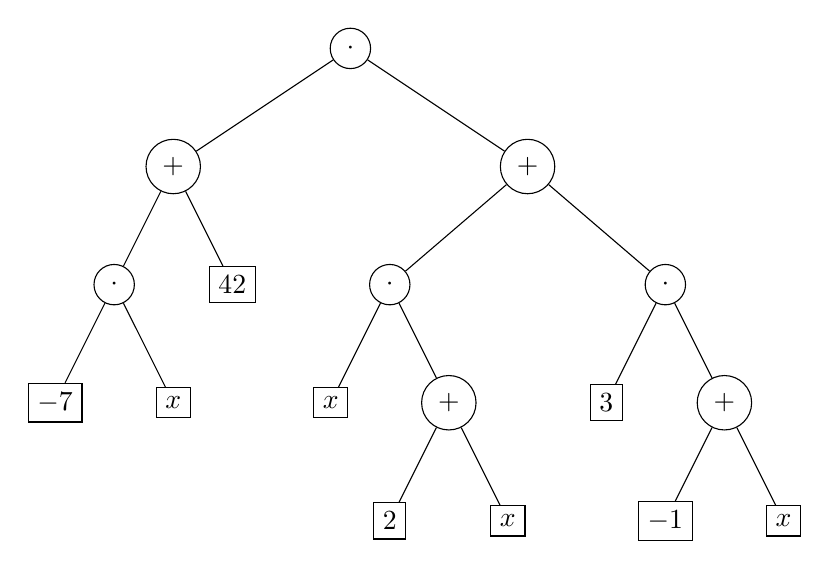
\begin{tikzpicture}
\node [circle,draw] {$\cdot$}
  child {
    node [circle,draw,xshift=-15mm] {$+$}
    child {
      node [circle,draw] {$\cdot$}
      child {node [draw]{$-7$}}
      child {node [draw]{$x$}}
    }
    child {node [draw] {$42$}}
  }
  child {
    node [circle,draw,xshift=15mm] (M) {$+$}
    child {
      node [circle,draw,xshift=-10mm]{$\cdot$}
      child {node [draw]{$x$}}
      child {
        node [circle,draw]{$+$}
        child {node [draw] {$2$}}
        child {node [draw] {$x$}}
        }
      }
    child {
      node [circle,draw,xshift=10mm]{$\cdot$}
      child {node [draw] {$3$}}
      child {
        node [circle,draw] {$+$}
        child {node [draw] {$-1$}}
        child {node [draw] {$x$}}
        }
    }
  };
\end{tikzpicture}
\end{center}
\caption{Il polinomio $P = \enclose{(-7)\cdot x + 42}\cdot(x\cdot (2+x) + 3\cdot(-1+x))$
rappresentato come albero di valutazione.}
\label{fig:49389}%
\end{figure}
Le espressioni polinomiali possono essere sommate e moltiplicate tra loro 
per ottenere nuove espressioni. 
Come comoda notazione si utilizzano le potenze intere per 
denotare un prodotto ripetuto $n$ volte: $x^n = x\cdots x$.

Diremo che due espressioni sono \emph{equivalenti} se è possibile trasformare 
una nell'altra utilizzando le proprietà valide negli anelli abeliani: 
proprietà associativa 
e commutativa per somma e prodotto, proprietà distributiva, elementi 
neutri $1\cdot x = x$, $0 + x = x$.
Inoltre se un ramo dell'espressione non contiene la variabile $x$ è possibile valutare 
(nell'anello $A$) le operazioni e sostituire l'intero ramo con il 
risultato di tali operazioni (e viceversa).

In particolare se abbiamo una qualunque espressione possiamo sviluppare tutti i prodotti
mediante la proprietà distributiva e poi riassociare i termini 
con le stesse potenze di $x$, ad esempio:
\begin{align*}
P &= \enclose{(-7)\cdot x+42}\cdot(x\cdot (2 + x)
+ 3\cdot(-1+x))\\
&= \enclose{(-7)\cdot x + 42}\cdot (2x+x^2-3+3x) \\
% (42-7x)  *  (-3 + 5x + x^2)
&= 126 + 231 x + 7 x^2 - 7 x^3
\end{align*}
In generale si otterrà una espressione polinomiale che diremo 
essere in \emph{forma canonica}:
\[
  P = a_0 + a_1 x + a_2 x^2 + \dots + a_n x^n
       = \sum_{k=0}^n a_k x^k.
\]
Dunque ogni espressione polinomiale è equivalente ad una 
espressione polinomiale in forma canonica. 

Se due espressioni polinomiali sono equivalenti 
diremo che rappresentano lo stesso \emph{polinomio}%
\mymargin{polinomio}%
\index{polinomio}.
Se $A$ è un anello denoteremo con 
$A[x]$ \index{$\KK[x]$}\index{$A[x]$}%
l'insieme di tutti i polinomi con coefficienti in $A$ e variabile $x$. 
Formalmente $A[x]$ è il quoziente dell'insieme 
di tutte le espressioni polinomiali rispetto alla relazione di equivalenza
che abbiamo appena definito. 
Possiamo fare la somma e il prodotto di polinomi e queste operazioni 
rendono $A[x]$ anch'esso un anello.

Più esplicitamente se $P$ e $Q$ sono polinomi in forma canonica
\[
  P = \sum_{k=0}^n a_k x^k, \qquad Q = \sum_{k=0}^m b_k x^k
\]
si avrà:
\[
  P + Q = \sum_{k=0}^{N} (a_k+b_k) \cdot x^k
\]
dove $N$ è il più grande tra $n$ e $m$ e si intende che $a_k=0$ per $k>n$ e 
$b_k=0$ per $k>m$.
Se $t\in A$ avremo:
\[
  t P = \sum_{k=0}^n (ta_k)\cdot x^k.
\]
Per quanto riguarda il prodotto si avrà invece:
\begin{align*}
  P\cdot Q
  &= \enclose{\sum_{k=0}^n a_k x^k}\cdot \enclose{\sum_{j=0}^n b_j x^j}
  = \enclose{\sum_{k=0}^n a_k \enclose{\sum_{j=0}^m b_j x^j} x^k} \\
  &= \enclose{\sum_{k=0}^n \sum_{j=0}^m a_k b_j x^{j+k}}
  = \sum_{s=0}^{m+n} \enclose{\sum_{j=0}^s a_j b_{s-j}} x^s.
\end{align*}

Le formule per la somma e il prodotto dei polinomi in forma canonica 
possono essere applicate ad ognuna delle proprietà di anello per dimostrare
che polinomi equivalenti hanno la stessa forma canonica e che quindi 
due espressioni polinomiali sono equivalenti se e solo se i coefficienti 
della loro forma canonica coincidono.
In pratica i polinomi a coefficienti in $A$ sono 
rappresentati dai coefficienti delle loro forme canoniche che 
non sono altro che sequenze finite:
\begin{align*}
  A[x] 
  &= \{\sum_{k=0}^n a_k x^k\colon a_k\in A, n\in \NN\}\\
  &\approx A^\NN_c 
  = \ENCLOSE{\vec a \in A^\NN\colon \ENCLOSE{k\in \NN\colon \vec a(k)\neq 0} \text{ è finito}}.  
\end{align*}

Se il polinomio $P$ si scrive in forma canonica
\[
  P = \sum_{k=0}^n a_k x^k
\]
se $n>0$ possiamo supporre che il coefficiente $a_n$ sia diverso da $0$ 
perché altrimenti potremmo rimuovere il termine corrispondente e ridurci 
ad una somma di $n-1$ termini. 
In tal caso diremo che il polinomio $P$ ha \emph{grado}%
\mymargin{grado}%
\index{grado} $n$.
\index{polinomio!grado}%
\index{grado!polinomio}% 
Se $n=0$ diremo anche che il polinomio è costante.
Se $n=0$ e $a_n=0$ diremo che $P$ è il polinomio \emph{nullo}.
I polinomi costanti non nulli hanno grado pari a $0$, mentre il polinomio nullo, 
per convenzione, diremo avere grado $-\infty$ (questa definizione ha senso se si pensa 
al grado di un polinomio come al più piccolo numero per cui tutti i coefficienti di
indice maggiore a lui sono nulli).

Finora abbiamo definito il polinomio come una classe di equivalenza di 
espressioni polinomiali. 
Se prendiamo una espressione $P$ e al posto della variabile $x$ 
mettiamo un elemento $a$ dell'anello $A$ (o di qualunque anello che estende 
$A$) allora possiamo valutare tutte le operazioni (somme e prodotti) ed 
ottenere un risultato nell'anello scelto: il risultato 
ottenuto si indica con $P(a)$ (stessa notazione utilizzata per le funzioni).
Se $P$ è un polinomio nella variabile $x$ la funzione $x\mapsto P(x)$ 
può essere chiamata \emph{funzione polinomiale}%
\mymargin{funzione polinomiale}%
\index{funzione!polinomiale} e si indica usualmente 
con con lo stesso nome $P$ dato al polinomio. Sarà il contesto a dirci 
se con $P$ si intende il polinomio (l'espressione) o la funzione.

Come già anticipato è utile tenere separato il concetto di polinomio da quello di 
funzione polinomiale in quanto lo stesso polinomio può essere valutato su diversi 
anelli (ad esempio nel corso di geometria si potrà sostituire
la variabile $x$ di un polinomio con una matrice, 
e nell'ultimo capitolo di questi appunti 
sostituiremo la $x$ con un operatore differenziale).

Proseguiremo con la trattazione dei polinomi 
nel capitolo~\ref{ch:ancora_polinomi}.

\section{coefficienti binomiali}
\label{ch:binomiale}

Capiterà spesso di imbattersi in alcuni polinomi particolari, che vengono 
a volte chiamati \emph{prodotti notevoli}%
\mymargin{prodotti notevoli}%
\index{prodotto!notevole}. 
Di fondamentale iportanza quelli di grado 2:
\[
  (x+1)\cdot(x-1) = x^2-1, \qquad (x+1)^2 = x^2+2x + 1.
\]
Ma anche quelli di grado $n$:
\[
  (x-1)\cdot \sum_{k=0}^{n-1} x^k
  = \sum_{k=0}^{n-1} x^{k+1} - \sum_{k=0}^n x^k = x^n - 1
\]
e, mettendo $-x$ al posto di $x$ e cambiando di segno:
\[
  (x+1)\cdot \sum_{k=0}^{n-1} (-1)^k x^k
  = 1 + (-1)^n x^n.
\]

Le potenze del binomio $x+1$ sono decisamente rilevanti. 
Se scriviamo il polinomio $(x+1)^n$ in forma canonica:
\[
  (x+1)^n = \sum_{k=0}^n a_k x^k  
\]
saremmo interessati a calcolare il valore
dei coefficienti $a_k$. 
Innanzitutto gli diamo un nome: questi coefficienti vengono chiamati 
\emph{coefficienti binomiali}%
\mymargin{coefficienti binomiali}%
\index{coefficienti binomiali}
\index{binomio!coefficienti}%
e si denotano nel modo seguente:%
\footnote{%
I coefficienti binomiali nell'ambito del calcolo combinatorio 
vengono anche chiamati \emph{combinazioni}
e denotati con il simbolo $C_{n,k} = {n \choose k}$.
La coincidenza tra le combinazioni e i coefficienti binomiali 
è espressa nel teorema~\ref{th:combinatoria}.
}%
\[
    a_k = {n \choose k}.
\]

Non è difficile convincersi che se sviluppiamo il binomio $(x+y)^n$
si ottengono gli stessi coefficienti dunque
in generale vale la seguente formula per la \emph{potenza del binomio}%
\mymargin{potenza del binomio}%
\index{potenza!del binomio}:
\index{binomio!potenza}% 
\begin{equation*}
  (x+y)^n = \sum_{k=0}^n {n \choose k} x^k y^{n-k}. 
\end{equation*}

Per determinare il valore effettivo dei coefficienti 
binomiali si utilizza usualmente il seguente.
  
\begin{theorem}[triangolo di Tartaglia]
\mymark{*}%
\label{th:tartaglia}%
Per ogni $n\in \NN$ e $k \in \NN$ con $1 \le k \le n$ si ha
\[
  {n+1 \choose k} =
      {n \choose k-1} + {n \choose k}
\]
mentre
\[
  {n+1 \choose 0} = 1 = {n+1 \choose n+1}
\]
\end{theorem}
  %
  \begin{proof}
  Infatti si ha 
  \begin{align*}
    \sum_{k=0}^{n+1} {n+1 \choose k} x^k
    &= (1+x)^{n+1} 
    = (1+x)\cdot \sum_{k=0}^n {n \choose k} x^k \\
    &= \sum_{k=0}^n {n\choose k} x^k 
    + \sum_{k=0}^n {n\choose k} x^{k+1}\\
    &= \sum_{k=0}^n {n\choose k} x^k 
    + \sum_{k=1}^{n+1} {n\choose k-1} x^{k}\\
    &= {n\choose 0} x^0 
      + \sum_{k=1}^n \Enclose{{n\choose k} + {n\choose k-1}} x^k
      + {n \choose n} x^{n+1}.
    \end{align*}
  Per l'unicità della forma canonica dei polinomi 
  i coefficienti corrispondenti devono essere uguali e quindi 
  troviamo
  \[
  {n+1 \choose 0} = {n \choose 0}, \qquad 
  {n+1 \choose k} = {n \choose k} + {n \choose k-1}, \qquad 
  {n+1 \choose n+1} = {n \choose n}.
  \]

  Si può facilmente verificare che  ${0 \choose 0} = 1$ 
  e questo conclude la dimostrazione.
  \end{proof}
  
  In base al teorema precedente i coefficienti binomiali si possono
  elencare come nella tabella~\ref{tab:binomiali}:
  ogni riga inizia e finisce con il numero $1$
  e ogni termine intermedio coincide con la somma dei
  due termini nella riga precedente sopra e
  a sinistra del numero considerato.
  
  \begin{table}
  \begin{tabular}{c|ccccccccc}
  $\displaystyle{n \choose k}$& 0 & 1 & 2 & 3 & 4 & 5 & 6 & $k$ &\\ \hline
    0 & 1 &   &   &   &   &   &   & &\\
    1 & 1 & 1 &   &   &   &   &   & &\\
    2 & 1 & 2 & 1 &   &   &   &   & &\\
    3 & 1 & 3 & 3 & 1 &   &   &   & &\\
    4 & 1 & 4 & 6 & 4 & 1 &   &   & &\\
    5 & 1 & 5 & 10& 10& 5 & 1 &   & &\\
    6 & 1 & 6 & 15& 20& 15& 6 & 1 & &\\
  $n$ &$\vdots$&&   &   &   &   &   & $\ddots$ &
  \end{tabular}
  \caption{Il triangolo di Tartaglia (o di Pascal):
  ogni numero è la somma dei due numeri che si trovano 
  nella riga precedente sopra e immediatamente a sinistra.}
  \label{tab:binomiali}
  \end{table}
  
  \begin{theorem}[formula per i coefficienti binomiali]
  \mymark{***}%
  Se $n\in \NN$ e $k\in \NN$, $k\le n$
  si ha 
  \[
  {n \choose k}  
  = \frac{n!}{k!(n-k)!}.  
  \]
  \end{theorem}
  %
  \begin{proof}
  Lo dimostriamo per induzione su $n$.
  Per $n=0$ sappiamo che ${0 \choose 0} = 1$ che 
  è ugule a $\frac{0!}{0!0!}$.
  Utilizziamo il teorema~\ref{th:tartaglia}.
  Se $k=0$ o $k=n$ sappiamo che ${n \choose k}=1$ che coincide 
  con la formula enunciata. 
  Per gli altri casi, supponendo per induzione che la formula sia 
  vera per un certo $n\in \NN$ si ha: 
  \begin{align*}
   {n+1 \choose k} 
   &= {n \choose k} + {n \choose k-1}
   =  \frac{n!}{k!(n-k)!} + \frac{n!}{(k-1)!(n-k+1)!} \\
   &= \frac{n!(n-k+1) + n! k}{k!(n-k+1)!}
   = \frac{n!(n+1)}{k!(n+1-k)!} \\
   &= \frac{(n+1)!}{k!(n+1-k)!}
  \end{align*}
  che è quanto dovevamo dimostrare.
\end{proof}

Si osservi che risulta, per ogni $n\in \NN$:
\[
  {n \choose 1} = {n \choose n-1} = n.
\]
  
\begin{exercise}
  Provare che
  \[
   \sum_{k=0}^n {n \choose k} = 2^n.
  \]
\end{exercise}  
  
\section{frazioni e numeri razionali}

Così come abbiamo esteso i numeri naturali affinché l'operazione di addizione abbia 
una operazione inversa (la sottrazione) in modo simile possiamo estendere l'insieme 
dei numeri interi in modo che anche la moltiplicazione abbia una operazione inversa 
(la divisione).

Per fare questo consideriamo i ``riscalamenti'' su $\ZZ$. Dati $p,q\in \ZZ$ se 
$q\neq 0$ possiamo considerare la funzione $s$ definita sui multipli di $q$ 
tale che $s(k\cdot q) = k\cdot p$ per ogni $k\in \ZZ$.
Si tratta del riscalamento che manda $q$ in $p$ e lo possiamo identificare 
con la frazione $\frac{p}{q}$ (formalmente una frazione non è altro che una 
coppia di interi $(q,p)$ con $q\neq 0$).
Osserviamo però che frazioni diverse possono rappresentare lo stesso riscalamento 
nell'intersezione dei loro domini. 
Infatti i due riscalamenti rappresentati dalle frazioni $\frac{p}{q}$ e $\frac{p'}{q'}$
sono definiti entrambi sul numero $q\cdot q'$ e si ha
$\frac{p}{q}(q\cdot q') = p\cdot q'$ e  $\frac{p'}{q'}(q\cdot q')=p'\cdot q$ per cui se $p\cdot q'=p'\cdot q$
i due riscalamenti coincidono in un punto. Ma se coincidono in un punto coincidono 
in tutti i punti in cui sono entrambi definiti. 
Diremo in tal caso che le due frazioni sono equivalenti e scriveremo 
\[
  \frac{p}{q} \sim \frac{p'}{q'} \iff p\cdot q'=p'\cdot q.  
\]

I \emph{numeri razionali} non sono altro che le frazioni identificate 
a meno di equivalenza:
\[
  \QQ = ((\ZZ\setminus\ENCLOSE{0})\times \ZZ)/\sim.
\]

La moltiplicazione tra numeri razionali può essere definita tramite la composizione 
dei riscalamenti:
\[
  \frac{p}{q}\enclose{\frac{p'}{q'} (q\cdot q')} = \frac{p}{q}(p'\cdot q) = p\cdot p'
\]
da cui 
\[
 \frac{p}{q} \cdot \frac{p'}{q'} = \frac{p\cdot p'}{q\cdot q'}.  
\]
Si verifica facilmente che questa definizione \emph{passa al quoziente} 
nel senso che il prodotto di frazioni equivalenti è equivalente al prodotto 
delle frazioni. 
Dunque la moltiplicazione è ben definita su $\QQ$.

Le frazioni del tipo $\frac{q}{q}$ sono tutte equivalenti tra loro e rappresentano 
l'elemento neutro della moltiplicazione.
Le frazioni del tipo $\frac{p}{1}$ rappresentano la moltiplicazione per $p\in\ZZ$ 
e quindi identificano i numeri interi $\ZZ$ all'interno di $\QQ$.
Per poter estendere l'addizione da $\ZZ$ a $\QQ$ in modo da preservare 
la proprietà distributiva sarà quindi necessario che 
si abbia 
\[
  \enclose{\frac{p}{q}+\frac{p'}{q'}} (q\cdot q') = \frac{p}{q}(q\cdot q') + \frac{p'}{q'}(q\cdot q')
  = p\cdot q' + p'\cdot q
\]
da cui
\[
  \frac{p}{q} + \frac{p'}{q'} = \frac{p\cdot q'+p'\cdot q}{q\cdot q'}.  
\]
E' facile verificare che anche questa definizione \emph{passa al quoziente}
ovvero che la somma di frazioni equivalenti è equivalente alla somma delle 
frazioni dunque anche l'addizione in questo modo è ben definita su $\QQ$.

Abbiamo quindi esteso l'addizione e la moltiplicazione da $\ZZ$ a $\QQ$
e ora, su $\QQ$.
Rispetto all'addizione $\QQ$ risulta essere un gruppo commutativo (come lo era $\ZZ$)
in quanto ogni frazione $\frac{p}{q}$ ha come opposto $\frac{-p}{q}$ 
e l'addizione rimane associativa e commutativa.

Inoltre in $\QQ$ ogni elemento diverso da $0$
\footnote{$0\in \ZZ$ si identifica in $\QQ$ con la classe di equivalenza 
delle frazioni del tipo $\frac{0}{q}$ e $1$ è rappresentato 
dalle frazioni del tipo $\frac{q}{q}$.}
ha anche un inverso moltiplicativo, infatti se $p\neq 0$ e $q\neq 0$ si ha:
\[
 \frac{p}{q}\cdot \frac{q}{p} = \frac{p\cdot q}{q\cdot p} \sim \frac{1}{1}.  
\]
Dunque $\QQ\setminus\ENCLOSE{0}$ risulta essere a sua volta un gruppo 
moltiplicativo.

In maniera naturale diremo che una frazione $\frac{p}{q}$ è non-negativa 
se, visto come riscalamento, manda gli interi non-negativi in interi non-negativi. 
Questo succede se $p$ e $q$ non hanno segno opposto, ovvero se $p\cdot q\ge 0$.
Possiamo quindi definire un ordinamento su $\QQ$ 
ponendo $x\le y$ se $y-x$ è non-negativo e cioè, visto sulle frazioni,
\[
 \frac{p}{q} \le \frac{p'}{q'} \iff \frac{p'\cdot q-p\cdot q'}{q\cdot q'}\ge 0 
 \iff (p'\cdot q-p\cdot q')\cdot q\cdot q' \ge 0. 
\]
Questo ordinamento estende quello di $\ZZ$ e rende sia il gruppo additivo $\QQ$
che il gruppo moltiplicativo $\QQ^+ = \ENCLOSE{q\in \QQ\colon q>0}$
un gruppo totalmente ordinato. 

In effetti risulta che $\QQ$ è il nostro primo esempio 
di campo ordinato, in base alla seguente definizione.

\begin{definition}[campo]
  \label{def:campo}%
  Diremo che $\KK$ è un campo se $\KK$ è un anello commutativo con unità 
  (definizione~\ref{def:anello})
  e se ogni $x\in \KK$, $x\neq 0$ ha un inverso moltiplicativo cioè 
  esiste $y\in \KK$ tale che $x\cdot y = 1$.
  L'inverso moltiplicativo si chiama anche \emph{reciproco}%
\mymargin{reciproco}%
\index{reciproco}.
  Se $y\neq 0$ denotiamo con $x/y$ o $\frac x y$ il prodotto 
  di $x$ con il reciproco di $y$. 
  Questa operazione si chiama \emph{divisione}%
\mymargin{divisione}%
\index{divisione}.

  Se $\KK$ è anche totalmente ordinato da una relazione $\le$
  (definizione~\ref{def:ordine})
  e se valgono anche le seguenti proprietà:
  \[
  a \le b \implies a+c\le b+c, \qquad 
  a,b\ge 0 \implies a\cdot b \ge 0
  \]
  diremo che $\KK$ è un \emph{campo ordinato}%
\mymargin{campo ordinato}%
\index{campo!ordinato}.
\end{definition}

Sull'insieme numerico $\QQ$ le operazioni di addizione e moltiplicazione 
sono dunque entrambe invertibili (salvo la moltiplicazione per zero). 
Questo è molto utile perché ci permette di risolvere tutte le equazioni lineari
della forma :
\[
  mx + q = 0  
\]
quando $m\neq 0$. Infatti la funzione $f(x) = mx+q$ è una composizione 
di una moltiplicazione $x\mapsto mx$ con una somma $y\mapsto y+q$ e la sua funzione
inversa si trova quindi invertendo le due operazioni: 
\[
  mx = -q, \qquad x = \frac{-q}{m}.  
\]

Ci sono però altre equazioni che vorremmo risolvere ma che non hanno soluzione su 
$\QQ$. 
L'esempio più semplice (scoperto da Pitagora) è l'equazione $x^2=2$.
%
\begin{theorem}[irrazionalità di $\sqrt 2$]
  \mymark{**}%
  \label{th:pitagora}%
  L'equazione $x^2=2$ non ha soluzioni in $\QQ$.
  \end{theorem}
  %
  \begin{proof}
  \mymark{*}%
  Supponiamo $x\in \QQ$ sia una soluzione di $x^2=2$.
  Allora si potrà scrivere $x=p/q$ con $p\in \ZZ$ e $q\in \NN$, $q\neq 0$.
  Possiamo anche supporre che la frazione $p/q$ sia ridotta ai minimi
  termini cioè che $p$ e $q$ non abbiano fattori in comune.
  Moltiplicando l'equazione
  $(p/q)^2=2$ per $q^2$ si ottiene $p^2 = 2 q^2$.
  Risulta quindi che $p^2$ è pari.
  Ma allora anche $p$ è pari (perché il quadrato di un dispari è dispari).
  Ma se $p$ è pari allora $p^2$ è multiplo di quattro.
  Ma allora anche $2q^2$ è multiplo di quattro e quindi $q^2$ è pari.
  Dunque anche $q$ è pari. Ma avevamo supposto che $p$ e $q$ non avessero
  fattori in comune quindi questo non può accadere.
\end{proof}

\subsection{valore assoluto}

\begin{definition}[valore assoluto]
\mymark{***}
Se $\KK$ è un campo totalmente ordinato (ad esempio $\KK=\QQ$ o, come vedremo, $\KK=\RR$)
definiamo il \emph{valore assoluto}%
\mymargin{valore assoluto}%
\index{valore!assoluto} $\abs{x}$ di un numero $x\in \KK$ nel seguente modo:
\[
\abs{x} =
\begin{cases}
  x & \text{se $x\ge 0$}, \\
  -x & \text{se $x<0 $}.
\end{cases}
\]
\end{definition}
  
\begin{proposition}[proprietà del valore assoluto]
\mymark{**}
Si ha
\begin{enumerate}
\item $\abs{x}\ge 0$ (positività)
\item $\big\lvert\abs{x}\big\rvert = \abs{x}$ (idempotenza)
\item $\abs{-x} = \abs{x}$ (simmetria)
\item $\abs{x\cdot y} = \abs{x}\cdot \abs{y}$ (omogenità)
\item $\abs{x+y} \le \abs{x} + \abs{y}$ (convessità)
\item $\abs{x-y} \le \abs{x-z} + \abs{z-y}$ (disuguaglianza triangolare)
\item $\big\lvert\abs{x}-\abs{y}\big\rvert \le \abs{x-y}$ (disuguaglianza triangolare inversa)
\end{enumerate}
Useremo inoltre spesso la seguente equivalenza (valida
anche con $<$ al posto di $\le$). Se $r\ge 0$ allora
\[
  \abs{x-y} \le r
  \iff
  y - r \le x \le y + r.
\]
\end{proposition}
%
\begin{proof}
\mymark{*}
Positività, idempotenza, simmetria e omogenità sono immediate conseguenze della definizione.

Dimostriamo ora l'ultima osservazione.
Se $x\ge y$ allora $x-y\ge 0$ e quindi $\abs{x-y} \le r$ è
equivalente a $x-y\le r$ cioè $x\le y+r$.
Se $x<y$ allora $x-y<0$ e quindi $\abs{x-y} \le r$ è
equivalente a $y-x \le r$ cioè $x\ge y-r$.
Viceversa se $y-r \le x \le y+r$ allora vale sia $x-y \le r$ che $y-x \le r$ e 
dunque $\abs{x-y}\le r$.

Osserviamo allora che per la precedente osservazione applicata
a $\abs{x-0} \le \abs{x}$ si ottiene
\[
  -\abs{x} \le x \le \abs{x}
\]
e sommando la stessa disuguaglianza con $y$ al posto di $x$ si
ottiene
\[
  -(\abs{x} + \abs{y}) \le x + y \le \abs{x} + \abs{y}
\]
che è equivalente alla proprietà di convessità:
\[
  \abs{x+y} \le \big\lvert\abs{x} + \abs{y}\big\rvert = \abs{x} + \abs{y}.
\]

Ponendo $y=z-x$ nella disuguaglianza precedente, si ottiene
\[
  \abs{z} \le \abs{x} + \abs{z-x}
\]
da cui
\[
  \abs{z} - \abs{x} \le \abs{z-x}.
\]
Scambiando $z$ con $x$ si ottiene la disuguaglianza opposta
e mettendole assieme si ottiene
la disuguaglianza triangolare inversa:
\[
\big\lvert \abs{z}-\abs{x} \big\rvert  \le \abs{z-x}.
\]

La disuguaglianza triangolare segue dalla convessità:
\[
  \abs{x-y} = \abs{x-z + z-y} \le \abs{x-z} + \abs{z-y}.
\]
\end{proof}

Osserviamo che dal punto di vista geometrico
$\abs{x-y}$ rappresenta la \emph{distanza} tra i punti
$x$ e $y$.

\section{costruzione dei numeri reali}

Osserviamo che l'insieme 
\[
 A = \ENCLOSE{x\in \QQ \colon x^2 \le 2}  
\]
non ha massimo. 
Infatti se $x\in A$ non può essere $x^2=2$ (per il teorema~\ref{th:pitagora})
e quindi dovrà essere $x^2<2$. 
Ma possiamo dimostrare che se $x^2<2$ esiste $\eps>0$ tale per cui $(x+\eps)^2<2$. 
Infatti si ha $(x+\eps)^2 = x^2 + 2\eps x + \eps^2$
ma se $x^2<2$ certamente dovrà essere $x<2$ (altrimenti $x^2\ge 4$)
e quindi $x^2+2\eps x+\eps^2 < x^2+ 4\eps^2+\eps^2 = x^2+5\eps^2$.
Se ora scegliamo $\eps<1$ sappiamo che $\eps^2<\eps$ 
e quindi $x^2+5\eps^2 < x^2 + 5\eps$. 
E affinché sia $x^2 + 5\eps < 2$ è sufficiente scegliere 
$\eps < \frac{2-x^2}{5}$. 
In tal modo abbiamo dimostrato che se $x\in A$ allora esiste 
$\eps>0$ tale che $x+\eps \in A$. 
Questo significa che l'insieme $A$ non ha massimo.

L'idea è ora che una ipotetica soluzione positiva dell'equazione $x^2=2$ 
dovrebbe potersi approssimare, per difetto, con gli elementi dell'insieme $A$.
Allora vogliamo utilizzare l'insieme $A$ per rappresentare un tale ipotetico numero.

Procediamo dunque col definire (si ricordi la definizione~\ref{def:limitato}):
\[
\mathcal R = \ENCLOSE{A \in \mathcal P(\QQ)\colon A\neq \emptyset, \text{ $A$ superiormente 
limitato}}.
\]
Dati $A,B\in \mathcal R$ scriveremo $A\sim B$ 
se $A$ e $B$ hanno gli stessi maggioranti, ovvero
se per ogni $q\in \QQ$ si ha $q\ge A \iff q\ge B$.
Chiaramente $\sim$ è una relazione di equivalenza (vedi definizione~\ref{def:equivalenza})
l'insieme degli insiemi equivalenti ad $A$ si chiama 
classe di equivalenza e viene denotata con $\Enclose{A}_\sim$.
Possiamo quindi definire il quoziente
\[
  \RR = \mathcal R / \sim = \ENCLOSE{\Enclose{A}_\sim\colon A\in \mathcal R},
  \qquad 
  \Enclose{A}_\sim = \ENCLOSE{B\in \mathcal R\colon B\sim A}
\]
che chiameremo insieme dei \emph{numeri reali}%
\mymargin{numeri reali}%
\index{numeri!reali}.
L'idea di questa definizione è che i numeri reali 
possono essere identificati dalle loro approssimazioni 
per difetto tramite numeri razionali. 
Diverse approssimazioni, però, possono rappresentare 
lo stesso numero reale.

\begin{exercise}
  Si mostri che si ha $A \sim B \sim C$ se
  \[
  A = \ENCLOSE{1}, \qquad 
  B = \ENCLOSE{x\in \QQ\colon x<1}, \qquad
  C = \ENCLOSE{\frac{n}{n+1}\colon n\in \NN}.
  \]
\end{exercise}

\begin{exercise}
  Si mostri che si ha $A\sim B$ se
  \[
  A = \ENCLOSE{x\in \QQ\colon x^2<2}, \qquad
  B = \ENCLOSE{\frac{n}{10^k}\colon n\in \NN, k\in \NN, n^2 \le 2\cdot 100^k < (n+1)^2}.  
  \]
  Verificare che 
  \[
    B \supset \ENCLOSE{
      1,\frac{14}{100},\frac{141}{10000},\frac{1414}{1000000},
      \frac{14142}{100000000}}.
  \]
\end{exercise}

Dati $A,B\in\mathcal R$ definiamo $A+B=\ENCLOSE{a+b\colon a\in A, b\in B}$.
Chiaramente $A+B\in \mathcal R$ inoltre non è difficile dimostarare che 
se $A\sim A'$ e $B\sim B'$ si ha $A+B\sim A'+B'$.
Questo significa che è ben definita l'addizione su $\RR$ in modo che 
per ogni $A,B \in \mathcal R$ si abbia:
\[
\Enclose{A}_\sim + \Enclose{B}_\sim = \Enclose{A+B}_\sim.
\]
Ovviamente l'addizione su $\RR$ è associativa e commutativa in quanto 
queste proprietà valgono su $\QQ$ e di conseguenza su $\mathcal R$:
$(A+B)+C = \{ a+b+c\colon a\in A, b\in B, c\in C\} = A + (B+C)$ e 
$A+B = \{a+b\colon a\in A, b\in B\} = B+A$.
Visto che $A+\ENCLOSE{0} = A$ notiamo anche che $\Enclose{\ENCLOSE{0}}_\sim$ 
è elemento neutro dell'addizione.

Dato $A\in \mathcal R$ denotiamo con $A'$ l'insieme dei maggioranti di $A$.
Vogliamo dimostrare che $A$ e $A'$ contengono punti arbitrariamente vicini:
\begin{equation}\label{eq:48023775}
\forall \eps\in\QQ\colon (\eps >0 \implies \exists a \in A\colon \exists b\in A'\colon
b-a < \eps).
\end{equation}
Per fare ciò prendiamo qualunque $c\in A$ (visto che $A\neq \emptyset$)
e qualunque $q\in A'$ (visto che $A$ è superiormente limitato, $A'\neq \emptyset$).
L'insieme $I=\ENCLOSE{n\in \NN \colon c+n\eps\in A'}$
non è vuoto in quanto se $n>\frac{q-c}\eps$ si ha $c+n\eps>q$ ed essendo $q$ 
un maggiorante di $A$ anche $c+n\eps$ lo è.
Dunque per il buon ordinamento di $\NN$ (teorema~\ref{th:buon_ordinamento})
l'insieme $I$ ha minimo, che chiamiamo $k$.
Se $k=0$ significa che $c\in A'$ e posto $a=b=c$ si ottiene 
che \eqref{eq:48023775} è banalmente verificata.
Altrimenti prendiamo $b=c+k\eps$.
Per la scelta di $k$ sappiamo che $b\in A'$ e $c+(k-1)\eps$ non è un maggiorante di 
$A$. 
Ma allora esiste $a\in A$ tale che $a>c+(k-1)\eps$ da cui 
$b-a < \eps$ e \eqref{eq:48023775} è ancora verificata.

Possiamo ora osservare che posto $B=-A' = \{-x\in \QQ \colon x$ maggiorante di $A\}$
si ha $(A+B)\sim\ENCLOSE{0}$. 
I maggioranti di $\ENCLOSE{0}$ sono i $q\in \QQ$ con $q\ge 0$, 
vogliamo dimostrare che anche $A+B$ ha gli stessi maggioranti.
Ma se $a\in A$ e $b\in B$ risulta che $-b\ge a$ ovvero $a+b\le 0$ 
dunque $0$ è un maggiorante di $A+B$ e qualunque $q\ge 0$ lo è a maggior ragione.
Se invece $q<0$ per la proprietà \eqref{eq:48023775} esistono $a\in A$ 
e $-b\in A'$ (cioè $b\in B$) tali che $(-b)-a<-q$ cioè $a+b>q$. Dunque 
$q<0$ non è un maggiorante di $A+B$ e concludiamo che $A+B\sim\ENCLOSE{0}$.

Questo dimostra che dato qualunque $x\in \RR$ se $x=\Enclose{A}_\sim$
posto $y=\Enclose{-A'}$ si ha $x+y=\Enclose{0}_\sim$.
Dunque ogni $x\in \RR$ ha opposto $y$ che denoteremo 
con $y=-x$.

Abbiamo quindi dimostrato che $\RR$ è un gruppo rispetto all'operazione 
di addizione. L'ordinamento di $\QQ$ può essere facilmente esteso a $\RR$
definendo $\Enclose{A}_\sim \le \Enclose{B}_\sim$ se ogni maggiorante di $B$ 
è anche maggiorante di $A$. Questa definizione non dipende dalla scelta 
di $A$ e $B$ nella loro classe di equivalenza perché all'interno della classe di 
equivalenza l'insieme dei maggioranti 
non cambia.
Chiaramente $x\le x$, se $x\le y$ e $y\le x$ si ha $x=y$ 
e se $x\le y$, $y\le z$ si ha $x\le z$: dunque $\le$ è un ordinamento su $\RR$.
E' inoltre un ordinamento totale perché dati $x=\Enclose{A}_\sim$ e 
$y=\Enclose{B}$ se $x\neq y$ significa che l'insieme dei maggioranti 
di $A$ è diverso dall'insieme dei maggioranti di $B$. 
Supponiamo allora che esista $q$ che è maggiorante di $A$ 
ma non maggiorante di $B$ (se succede il viceversa basta scambiare $A$ e $B$).
In tal caso $B\ge A$ in quanto ogni maggiorante di $B$ deve essere maggiore 
di $q$ e quindi deve essere anche un maggiorante di $A$ da cui $x\le y$. 

L'ordinamento è compatibile con l'addizione perché se $\Enclose{A}_\sim 
\le \Enclose{B}_\sim$ e $A,B,C\in \mathcal R$ 
allora se $q$ è maggiorante di $B+C$ per ogni $c\in C$ si ha che $q-c$ 
è maggiorante di $B$ e dunque $q-c$ è anche maggiorante di $A$.
Ma allora $q$ è maggiorante di $A+C$. Dunque se $x\le y$ e $x,y,z\in \RR$ 
si ha $x+z\le y+z$ e $\RR$ è un gruppo ordinato.

\begin{definition}[ordinamento denso]
  \label{def:ordinamento_denso}%
  Un ordinamento $\le$ si dice essere
  \emph{denso}%
\mymargin{ordinamento denso}%
\index{denso} o \emph{divisibile} 
  se tra due punti distinti esiste sempre un punto intermedio:
  \[
   x < y \implies \exists c \colon x < c < y.
  \]
\end{definition}
  
L'ordinamento di $\RR$ è denso. Infatti se $x<y$ posto $y-x=\Enclose{A}_\sim$ 
sappiamo che ogni maggiorante di $A$ è maggiore o uguale a $0$.
Ma se ogni numero positivo fosse maggiorante di $A$ avremmo $A\sim\ENCLOSE 0$
che non è possibile in quanto $x\neq y$. Dunque esiste $q>0$ 
che non è maggiorante di $A$. 
Ma allora $y-x \ge \Enclose{\ENCLOSE q}_\sim > \Enclose{\ENCLOSE{\frac q 2}}_\sim = \eps > 0$
da cui $x<x+\eps<y$.

\begin{definition}[ordinamento continuo]
  \label{def:ordinamento_continuo}%
  Un ordinamento $\le$ su un insieme $X$ si dice essere
  \emph{continuo}%
\mymargin{ordinamento continuo}%
\index{continuo}
  \index{continuità!ordinamento}%
  \index{ordine!continuo}%
  (o \emph{Dedekind-completo})
  \index{Dedekind-completo}%
  \index{completo!Dedekind}%
  se dati comunque $A,B$ sottoinsiemi non vuoti di $X$
    tali che per ogni $a\in A$ e per ogni $b\in B$ risulta $a\le b$
    (concisamente scriveremo $A\le B$)
    allora esiste $c\in X$ tale che per ogni $a\in A$ e ogni $b\in B$ 
    si ha $a\le c \le b$ (concisamente $A\le c \le B$).
\end{definition}
  
A parole la condizione $A\le B$ 
si può esprimere dicendo che $A$ e $B$ sono separati, 
mentre la condizione $A\le c \le B$ 
si può esprimere dicendo che $c$ è un \emph{elemento di separazione}
tra $A$ e $B$. 
Allora la precedente definizione ci dice che un insieme ordinato
è \emph{continuo} ogni coppia di sottoinsiemi separati 
ammette un elemento di separazione.
In molti testi questa condizione viene chiamata \emph{completezza}
o, più precisamente, \emph{completezza di Dedekind}.
\index{completezza!di Dedekind}%
\index{Dedekind!completo}%

\begin{theorem}  
L'ordinamento di $\RR$ è continuo.
\end{theorem}
\begin{proof}
Siano dati $\mathcal A$ e $\mathcal B$ sottoinsiemi non vuoti di $\RR$ 
con $\mathcal A\le \mathcal B$. 
Possiamo definire
\[
  C = \bigcup\ENCLOSE{A\in \mathcal R\colon \Enclose{A}_\sim \in \mathcal A} 
    = \ENCLOSE{q\in \QQ\colon \exists A\in \mathcal R\colon 
    (\Enclose{A}_\sim \in \mathcal A) \land (q\in A)}.
\]
Preso qualunque $a=\Enclose{A}_\sim \in \mathcal A$ risulta 
ovviamente $A\subset C$. In particolare $C$ non è vuoto.
Mentre se $b=\Enclose{B}_\sim \in \mathcal B$ 
preso qualunque $q\in C$ si ha $q\in A$ per un qualche $A$ tale che 
$\Enclose{A}_\sim = a\in \mathcal A$.
Ma visto che $a\le b$, ogni maggiorante di $B$ è anche maggiorante di $A$.
In particolare preso un qualunque $r$ maggiorante di $B$
risulta che $r$ è un maggiorante di $C$.
Allora $C\in \mathcal R$ e posto $c=\Enclose{C}_\sim$ 
risulta che ogni maggiorante di $C$ è maggiorante di 
ogni $A$ con $\Enclose{A}_\sim \in \mathcal A$ mentre 
ogni maggiorante di un qualunque $B$ con $\Enclose{B}_\sim\in \mathcal B$ 
è anche un maggiorante di $C$.
Questo significa che $c\ge a$ per ogni $a\in A$ 
e $b\ge c$ per ogni $b\in B$: la dimostrazione è conclusa.
\end{proof}

Ad ogni $q\in \QQ$ si può associare l'elemento $\Enclose{\ENCLOSE q}_\sim$ 
di $\RR$. Ovviamente se $q\neq s$ in $\QQ$ allora $\ENCLOSE{q}$ 
ed $\ENCLOSE{s}$ non hanno gli stessi maggioranti e quindi si ottengono 
elementi distinti di $\RR$. Identificando $q$ con $\Enclose{\ENCLOSE q}_\sim$ 
possiamo quindi pensare che $\QQ \subset \RR$.

Prendiamo però l'insieme $A=\{x\in \QQ\colon x^2<2\}$.
Se fosse $A\sim \ENCLOSE q$ per qualche $q\in \QQ$ dovremmo 
concludere che $q$ è un maggiorante di $A$ e che ogni $s<q$ 
non è maggiorante di $A$. 
Ma allora dovrebbe essere $q^2\le 2$ perché se fosse $q^2>2$
potremmo trovare $s<q$ tale che anche $s^2>2$ 
(basta notare che $q<2$ e prendere $s=q-\eps$ con $\eps>0$, $\eps<1$, 
$\eps<\frac{q^2-2}{4}$ così $s^2=(q-\eps)^2 > q^2-2\eps q > q^2-4\eps
> q^2-(q^2-2) = 2$).
Dunque $\RR\neq \QQ$, l'elemento $x=[A]_\sim$ di $\RR$ sarà 
proprio quello che chiameremo $\sqrt 2$ e vedremo che 
risolverà l'equazione $x^2=2$. 

\section{proprietà assiomatiche dei numeri reali}
\label{sec:reali}

Nel paragrafo precedente abbiamo dimostrato che esiste un insieme 
$\RR$ su cui è definita una operazione di addizione
e un ordinamento che rendono $\RR$ un gruppo totalmente ordinato,
denso e continuo (definizioni~\ref{def:ordine}, \ref{def:ordinamento_denso},
\ref{def:ordinamento_continuo}). 

Come al solito d'ora in poi non guarderemo più come è stato definito $\RR$ 
ma utilizzeremo solamente le proprietà appena esposte. 
Potremmo anche pensare che $\RR$ debba esistere per assioma, 
evitando quindi di dover esibire la costruzione fatta nel capitolo precedente.


\subsection{estremo superiore}

\begin{definition}%
  Sia $R$ un insieme ordinato (in particolare pensiamo all'insieme $\RR$ 
  dei numeri reali).
  \mymark{***}%
  Sia $A \subset R$.
  Se $A$ ha un maggiorante (cioè esiste $x\in R$ tale che $x\ge A$, definizione~\ref{def:minorante})
  diremo che $A$ è \emph{superiormente limitato},
  se $A$ ammette un minorante diremo che $A$ è \emph{inferiormente limitato},
  \index{superiormente!limitato}%
  \index{inferiormente!limitato}%
  \index{limitato!superiormente}%
  \index{limitato!inferiormente}%
  se $A$ ammette sia maggiorante che minorante diremo che $A$ è 
  \emph{limitato}%
\mymargin{limitato}%
\index{limitato}.
  
  Se $x$ è minimo dei maggioranti di $A$ diremo che $x$ è
  \emph{estremo superiore}%
\mymargin{estremo superiore}%
\index{estremo!superiore}
  di $A$ se invece $x$ è massimo dei minoranti diremo che $x$ è
  \emph{estremo inferiore}%
\mymargin{estremo inferiore}%
\index{estremo!inferiore} di $A$:
  \begin{align*}
  \sup A &= \min \ENCLOSE{x\in R \colon x\ge A}, \\
  \inf A &= \max \ENCLOSE{x\in R \colon x \le A}.
  \end{align*}
  \index{$\sup$}%
  \index{$\inf$}%
  \index{sup}%
  \index{inf}%
\end{definition}

Osserviamo che se l'insieme $A$ è finito e non vuoto,
il massimo e il minimo esistono
sempre.
Se, ad esempio, non esistesse il massimo di $A$ significa che scelto
$x_k\in A$ esisterebbe sempre $x_{k+1}\in A$ con $x_{k+1} > x_k$ e quindi l'insieme
$A$ dovrebbe contenere infiniti punti $x_0,x_1, \dots, x_k,\dots $
Insiemi infiniti, invece, potrebbero non avere massimo/minimo.
Un esempio di insieme che non ha né massimo né minimo è
l'insieme $A = \ENCLOSE{x\in \RR\colon 0<x<1}$ infatti per ogni
$x\in A$ si ha $\frac x 2<x$, $\frac{1+x}{2}>x$
con $\frac x 2\in A$ e $\frac{1+x}{2}\in A$,
dunque nessun $x\in A$ può essere
massimo o minimo. L'insieme $B=\ENCLOSE{x\in \RR \colon 0\le x \le 1}$
ha invece massimo $\max B= 1$ e minimo $\min B=0$.

\begin{theorem}[esistenza del $\sup$]%
  \label{th:sup}%
  \mymark{**}%
  Sia $R$ un insieme dotato di un ordine totale e continuo
  (in particolare pensiamo a $R=\RR$).
  Se $A\subset R$ è un insieme non vuoto
  e superiormente limitato, allora esiste l'estremo superiore di $A$.
  Se $A\subset R$ è un insieme non vuoto e inferiormente limitato 
  allora esiste l'estremo inferiore di $A$.
  \end{theorem}
  %
  \begin{proof}
  \mymark{*}
  Consideriamo l'insieme dei maggioranti
  \[
  B = \ENCLOSE{ b\in R \colon b \ge A}.
  \]
  Per ipotesi $B$ è non vuoto e per come è definito risulta $A\le B$.
  Dunque dall'assioma di continuità (definizione~\ref{def:ordinamento_continuo}) 
  deduciamo l'esistenza di un numero $x\in \RR$
  tale che $A\le x \le B$. La prima disuguaglianza $A\le x$ ci dice che $x$ è un
  maggiorante e quindi $x\in B$, la seconda $x\le B$ ci dice che $x$ è il minimo
  di $B$ e quindi concludiamo che $x$ è il minimo dei maggioranti 
  ovvero l'estremo superiore di $A$.

  Dimostrazione analoga vale per l'estremo inferiore.
\end{proof}

L'esistenza del $\sup$ (o dell'$\inf$)
è in effetti una condizione equivalente all'assioma di continuità.
Infatti se $A\le B$ certamente $\sup A$, se esiste, è elemento 
di separazione tra $A$ e $B$.

\subsection{parte intera}

Se $R$ è un gruppo con operazione $+$ ed elemento neutro $0$, 
allora per ogni $x\in R$ si può definire 
il prodotto $n\cdot x$ con $n\in \NN$ come somma ripetuta:
Si pone $0\cdot x=0$ e per induzione $(n+1)\cdot x= n\cdot x + x$.
 
Il seguente risultato ci dice, informalmente, che non 
esistono quantità infinite (ma neanche infinitesime) in $\RR$.
%
\begin{theorem}[proprietà archimedea dei numeri reali]
\label{th:archimede}%
\mymark{**}%
\mymargin{proprietà archimedea}%
\index{proprietà!archimedea}%
  Sia $R$ un gruppo totalmente ordinato e completo
  (ad esempio $R=\RR$ sarà per noi il caso rilevante)
  con operazione $+$ ed elemento neutro $0$.
  Dati $x,y\in R$ con $x,y>0$ esiste $n\in \NN$ 
  tale che $n \cdot y > x$.

  A parole: per quanto piccolo possa essere $y>0$, 
  sommandolo a se stesso molte volte si arriva, 
  dopo un numero finito di passi, a superare 
  qualunque numero $x$ anche molto grande.
\end{theorem}
%
\begin{proof}
\mymark{*}
  Fissati $x,y\in R$, $x,y>0$ consideriamo l'insieme 
  \[
     A = \NN \cdot y = \ENCLOSE{n\cdot y\colon n\in \NN}.
  \]
  Basta dimostrare che $A$ non è superiormente limitato perché 
  in tal caso dato $x\in \RR$ esisterebbe $n\in \NN$ per cui $n\cdot y> x$.

  Chiaramente $A$ non è vuoto in quanto $0\in A$ dunque se $A$ 
  per assurdo fosse superiormente limitato esisterebbe 
  $m=\sup A$, $m\in R$. 
  Siccome $m$ è il minimo dei maggioranti di $A$
  e $m-y$ è più piccolo di $m$, allora $m-y$ non è un maggiorante. 
  Dunque deve esistere $n\in \NN$ tale che $ny>m-y$.
  Ma allora $(n+1)y = ny + y > m$ ed essendo $n+1\in \NN$ troviamo che $m$
  non poteva essere un maggiorante di $A$: assurdo.
\end{proof}

\begin{theorem}[parte intera]
\mymark{*}%
  Dato $x\in \RR$ esiste un unico $m\in \ZZ$ tale che $m-1 < x \le m$.
\end{theorem}
%
\begin{proof}
  Supponiamo per un attimo che sia $x > 0$
  e consideriamo l'insieme $A=\ENCLOSE{n \in \NN \colon n\ge x}$.
  Tale insieme non è vuoto per la proprietà archimedea 
  e dunque ammette minimo per il principio del buon ordinamento.
  Se $m=\min A$ risulta quindi $m\in \NN$ e $m-1< x \le m$.

  Se $x\le 0$ per la proprietà archimedea esiste $k\in \NN$ tale che 
  $k>-x$. Allora applichiamo il risultato precedente a $x+k$ e consideriamo 
  $m-k$ al posto di $m$.
\end{proof}

\begin{definition}[parte intera]
  \mymark{**}%
  \mymargin{parte intera}%
\index{parte!intera}%
  Dato $x\in \RR$ denotiamo con $\lfloor x\rfloor$ l'unico intero
  che soddisfa
  \mymargin{$\lfloor\cdot\rfloor$} %% *** non viene bene nell'indice!
  \[
    x - 1 < \lfloor x \rfloor \le x
  \]
  e denotiamo con $\lceil x \rceil = - \lfloor -x \rfloor$ l'unico intero che soddisfa (verificare!)
  \mymargin{$\lceil\cdot\rceil$} %% *** non viene bene nell'indice!
  \[
    x \le \lceil x \rceil < x + 1.
  \]
  Si ha dunque
  \[
    \lfloor x \rfloor \le x \le \lceil x \rceil
  \]
  con entrambe le uguaglianze che si realizzano quando $x\in \ZZ$.
  I due interi $\lfloor x \rfloor$ e $\lceil x \rceil$
  sono la migliore approssimazione intera di $x$ rispettivamente
  per difetto e per eccesso.
  L'intero più vicino ad $x$ (approssimazione per \emph{arrotondamento}%
\mymargin{arrotondamento}%
\index{arrotondamento})
  è
  \[
    \left\lfloor x + \frac 1 2 \right\rfloor
  \quad \text{ossia} \quad
    \left\lceil x-\frac 1 2 \right\rceil
  \]
  (le due espressioni differiscono solamente quando $x$ si trova nel punto medio tra 
  due interi consecutivi, nel qual caso la prima approssima per eccesso e la seconda 
  per difetto).
\end{definition}

In alcuni testi si usa la notazione $[x]$ per denotare la parte intera $\lfloor x \rfloor$ e si definisce
anche la \emph{parte frazionaria}
\[
  \ENCLOSE{x} = x - [x].
\]
Per evitare ambiguità con il normale utilizzo delle parentesi
non useremo queste notazioni.

\subsection{numeri decimali}
%
Le frazioni il cui denominatore è una potenza
di $10$ si chiamano frazioni decimali:
\[
  x = \frac{p}{10^d}, \qquad p\in \ZZ, d\in \NN.
\]
Tali frazioni si possono rappresentare
scrivendo il numero
intero $p$ e segnando un punto
\footnote{%
in Italia si preferisce utilizzare la virgola, ma
ci rassegnamo alla notazione anglosassone che ormai è
ubiqua in tutta la strumentazione elettronica.
}%
di separazione
prima della $d$-esima cifra a partire da destra.
Ad esempio scriveremo:
\[
  1.4142 = \frac{14142}{10^4}.
\]
In generale una frazione $\frac{p}{q}\in \QQ$
può essere scritta in forma decimale solamente
se, quando ridotta ai minimi termini,
risulta che $q$ non ha fattori primi diversi
da $2$ e $5$ (in quanto le potenze di dieci
hanno solo questi fattori).
In ogni caso le frazioni decimali sono dense in $\RR$
in quanto dato $x\in \RR$ per ogni $\eps>0$ esiste
$d\in \NN$ tale che $10^{-d}\le\eps$ e quindi
posto $p=\lfloor 10^d\cdot x + \frac 1 2\rfloor$
si avrà
\[
    \abs{\frac{p}{10^d} - x} \le \frac{1}{2\cdot 10^d} < \eps.
\]
In tal caso scriveremo
\mymargin{$\approx$}%
\index{$\approx$}
\[
  x \approx \frac{p}{10^d}.
\]
Ad esempio scriveremo
\[
  \frac 2 3 \approx 0.6667 = \frac{6667}{10^4}
\]
per intendere%
\footnote{%
Si osservi che in base alla definizione data sarebbe anche corretto 
scrivere $\frac 2 3 \approx 0.6666$ che però sarebbe una approssimazione 
peggiore. 
Questa ambiguità è necessaria se vogliamo evitare i casi 
limite in cui bisogna conoscere molte più cifre decimali di quelle richieste 
per capire qual è la migliore approssimazione.
}%
\begin{equation}\label{eq:approx_23}
\abs{\frac 2 3 - \frac{6667}{10^4}}<\frac{1}{10^4}.
\end{equation}
Nel calcolo scientifico ogni uguaglianza numerica è intesa nel 
senso precedente, se non specificato diversamente. 

Le frazioni non decimali si possono scrivere con uno sviluppo
decimale \emph{periodico}. 
Non useremo mai questa notazione
che ricordiamo solamente con un esempio.
Il numero
\[
  x = 12.34\overline{567}
    = 12.34567\overline{567}
\]
è la frazione che risolve l'equazione
\[
  \frac{100x - 1234}{1000}
  = 100x-1234.567
  \qquad
\enclose
{\frac{0.\overline{567}}{1000}
= 0.000\overline{567} }
\]
ovvero
\[
  1234567 - 1234 = 99900 \cdot x,
  \qquad x = \frac{1234567-1234}{99900}.
\]

\begin{exercise}
Dimostrare che vale~\eqref{eq:approx_23}.
\end{exercise}  

  
\subsection{isomorfismi di gruppi ordinati}

Intuitivamente si può ottenere $\RR$ a partire da una retta geometrica 
con lo stesso procedimento con cui si costruisce un righello.
Iniziamo col segnare
sulla retta un punto di riferimento che chiamiamo $0$, 
dopodiché osserviamo che
il punto $0$ (come ogni altro punto) divide la retta in due parti. In modo arbitrario
chiamiamo positivi i punti che si trovano da una parte e negativi i punti che
si trovano dall'altra parte. Sulla semiretta dei numeri positivi scegliamo, arbitrariamente,
un punto $1$. Il segmento compreso tra i punti $0$ e $1$ sarà la nostra unità di
misura.
L'addizione potrebbe essere definita utilizzando i movimenti rigidi.
Traslando il punto $1$ di una unità alla volta si ottengono, per iterazione, tutti i numeri naturali.
Traslando all'indietro si ottengono i numeri interi negativi. 
Assumendo che tra due punti qualunque esistano sempre punti intermedi (divisibilità) e
assumendo che suddividendo la retta in due parti esista sempre un punto di 
suddivisione (continuità) mostreremo come si può suddividere 
ogni segmento in $n$ parti uguali per ogni numero naturale $n$. 
In tal modo potremo ritrovare i numeri razionali e la moltiplicazione per un numero razionale.
Con una estensione crescente riusciremo quindi a definire la moltiplicazione 
tra numeri reali. 
Osserveremo poi che la struttura moltiplicativa dei numeri reali positivi soddisfa 
gli stessi assiomi della struttura additiva dei reali e che quindi la costruzione fatta 
per costruire la moltiplicazione si potrà ripetere identica per costruire l'elevamento a potenza.

\begin{theorem}[divisibilità]
  \label{th:divisibile}%
Se $R$ è un gruppo totalmente ordinato, denso e continuo
con operazione $+$ ed elemento neutro $0$
allora per ogni $y\in R$, $y\neq 0$ e per ogni $n\in \NN$, $n\neq 0$ 
esiste un unico $x\in R$ tale che $n\cdot x = y$.
\end{theorem}
\begin{proof}
Vogliamo innanzitutto dimostrare che 
\begin{equation}\label{eq:41095633}
  \forall y>0 \colon \exists x>0 \colon x+x \le y.
\end{equation}
Per la proprietà di densità sappiamo che esiste $z$ tale che 
$0<z<y$. 
Prendiamo $w=y-z$. Se $w\le z$ allora $w+w\le w+z=y$ e possiamo prendere $x=w$.
Altrimenti $z+z < w+z = y$ e possiamo prendere $x=z$.
%% Attenzione: la dimostrazione è delicata se il gruppo non è commutativo: bisogna 
%% fare attenzione all'ordine degli addendi! 

Ora dobbiamo dimostrare che per ogni $y\in R$ e per ogni $n\in \NN$, $n\neq 0$
esiste $x\in R$ tale che $n\cdot x=y$.
Per fissare le idee supponiamo che sia $y>0$: il caso $y=0$ è banale 
e se $y<0$ basterà applicare il risultato all'opposto $-y$.

Fissati $n\in \NN$, $n\neq 0$ e $y>0$ 
consideriamo allora gli insiemi:
\begin{align*}
  A &= \ENCLOSE{a\in R\colon a\ge 0, n\cdot a\le y},\\
  B &= \ENCLOSE{b\in R\colon n\cdot b\ge y}.
\end{align*}
Chiaramente si ha $a\le b$ per ogni $a\in A$ e $b\in B$ 
perché se $n\cdot a \le n\cdot b$ 
si può dedurre $a\le b$ (altrimenti si violerebbe
la proprietà $0\le a\le b \implies n\cdot a\le n\cdot b$ dimostrabile 
per induzione su $n\in \NN$).
Chiaramente $B\neq \emptyset$ in quanto $y\in A$ visto che $n\cdot y\ge y$ se 
$n\in \NN$, $n\neq 0$.
Meno ovvio dimostrare che $A\neq \emptyset$ per fare questo
dobbiamo considerare l'insieme 
$M=\ENCLOSE{m\in\NN\colon \exists x>0\colon m\cdot x\le y}$.
Ovviamente $1\in M$ e la proprietà~\eqref{eq:41095633}
ci dice che anche $2\in M$. 
Per dimostrare che $M=\NN$ basta allora dimostrare che 
se $n\in M$, $n\ge 2$ allora anche $n+1\in M$. 
Ma $n\in M$ significa che esiste $x>0$ tale che 
$n\cdot x\le y$. 
Per la proprietà~\eqref{eq:41095633} esiste anche $z>0$ 
tale che $z+z\le x$ e dunque 
\[
  (n+1)z \le (n+n)z = n(z+z)\le n\cdot x \le y.
\]
Visto che $M = \NN$ possiamo affermare che $A\neq \emptyset$.

Dunque $A\le B$ sono separati e non vuoti e per l'ipotesi di continuità di $R$ 
possiamo dedurre che esiste $y$ elemento di separazione: $A\le x \le B$.
Vogliamo dimostrare che $n\cdot x=y$.

Se fosse $n\cdot x<y$ vogliamo dimostrare che esiste $\eps>0$ 
tale che $n\cdot(x+\eps)<y$ e questo sarebbe assurdo perché
allora $x+\eps\in A$ e $x$ non sarebbe un maggiorante di $A$.
Affinché sia $n\cdot(x+\eps)<y$ basterà avere $n\cdot \eps < y-n\cdot x$.
Un tale $\eps>0_G$ esiste per quanto visto prima riguardo all'insieme 
$M$, mettendo $y-n\cdot x$ al posto di $y$.

Viceversa se fosse $n\cdot x>y$ vogliamo dimostrare che esiste $\eps>0$
tale che $n\cdot(x-\eps)>y$ e questo sarebbe assurdo perché
allora $x-\eps\in B$ e $x$ non sarebbe un minorante di $B$.
Anche in questo caso $\eps$ si trova facilmente imponendo 
la disequazione $n\cdot \eps < n\cdot x-y$.
\end{proof}

Ovviamente c'è un unico $x$ tale che $n\cdot x=y$ perché 
se $n\cdot z = n\cdot x$ si ha $n\cdot (z-x) = 0$ che è 
solo possibile quando $z=x$. Scriveremo $x=\frac{y}{n}$.

\begin{definition}[omomorfismo]%  
\label{def:omomorfismo}%
Siano $R$ ed $S$ due gruppi con operazione $*$ su $R$ e operazione $\circ$ su $S$.
Diremo che una funzione $\phi\colon R\to S$ è un \emph{omomorfismo}%
\mymargin{omomorfismo}%
\index{omomorfismo} se per ogni $x,y \in R$
\[
  \phi(x*y) = \phi(x)\circ \phi(y).
\]
\end{definition}

Sull'insieme $\RR$ è possibile definire la moltiplicazione per 
un numero $n$ naturale come somma ripetuta ed è possibile definire anche la divisione in $n$
parti uguali (teorema~\ref{th:divisibile}) e di conseguenza la moltiplicazione per ogni numero razionale.
Allora se fissiamo $u\in \RR$ che rappresenti l'unità, è possibile immergere $\QQ$ dentro $\RR$
associando $q\in \QQ$ al numero $q\cdot u\in \RR$.
E' quello che facciamo nel seguente.

\begin{lemma}
Sia $R$ un gruppo totalmente ordinato, denso, continuo e 
sia $\QQ$ il gruppo dei numeri razionali con l'operazione 
di addizione.
Allora fissato $u\in R$ esiste un unico omomorfismo $\phi\colon \QQ \to R$ tale che $\phi(1)=u$.

Se l'operazione su $R$ viene denotata con il simbolo di addizione $+$ 
l'omomorfismo $\phi$ può essere naturalmente denotato con il simbolo di moltiplicazione:
\[
   \phi(q) = q\cdot u
\]
cosicché la proprietà di omomorfismo è semplicemente la proprietà distributiva 
$(q+s)\cdot u = q\cdot u + s\cdot u$.

Denotiamo con $\QQ\cdot u$ l'immagine di $f$ ovvero
\[
  \QQ \cdot u = \ENCLOSE{q\cdot y \colon q\in \QQ}.
\] 
\end{lemma}
%
\begin{proof}
Usiamo il simbolo $+$ per denotare l'operazione del gruppo $R$ e chiamiamo $0$ 
l'elemento neutro di $R$.

\emph{Passo 1: definizione sugli interi.}
Chiaramente deve essere $\phi(0)=0$ in quanto $\phi(0) = \phi(0+0) = \phi(0)+\phi(0)$.
Inoltre $\phi(n+1) = \phi(n)+\phi(1) = \phi(n) + u$ e quindi per induzione
se $n\in \NN$ deve essere $\phi(n) = n\cdot u$ (addizione ripetuta).

Ma se $n\in \ZZ$ si ha $0=\phi(n+(-n)) = \phi(n)+\phi(-n)$ da cui 
$\phi(-n) = -\phi(n) = - n\cdot u$.
Dunque $\phi$ è univocamente definita su tutto $\ZZ$.

Ma ora ricordiamo che il teorema~\ref{th:divisibile} definisce $\frac{x}{n}$ 
per ogni $x\in R$ e ogni $n\in \NN$, $n\neq 0$. 
Osserviamo che la proprietà di omomorfismo ci dice che per ogni $q\in \QQ$ 
ed ogni $n\in \ZZ$ deve valere 
\[
  \phi(n\cdot q) = n \cdot \phi(q)  
\]
(lo si dimostra per induzione quando $n\in \NN$ e poi sugli altri $n\in \ZZ$ 
si utilizza la proprietà $\phi(-q) = -\phi(q)$ ottenibile anch'essa dalla proprietà 
di omomorfismo in quanto $q+(-q)=0$ e $\phi(0)=0$)
Allora la condizione $\phi(1)=u$ e la proprietà di omomorfismo ci dicono che 
dovrà essere $\phi(n) = n\cdot u$ per ogni $n\in \ZZ$.
Infatti $\phi(0) = 0$ in quanto $\phi(0+0)=\phi(0)+\phi(0)$
e si può sottrarre da ambo i membri l'opposto di $\phi(0)$.
Inoltre se $n\in \NN$ si ha $\phi(n+1)=\phi(n)+\phi(1)=\phi(n)+u$
dunque utilizzando l'induzione possiamo dimostrare 
che risulta 
\[
   \phi(n) = n\cdot u, \qquad \forall n\in \NN.
\]
Visto che $\phi(x-x)=0$ se vogliamo che valga la proprietà di omomorfismo
dovrà essere $phi(-x) = -\phi(x)$.
Dunque dovremo porre $phi(-n) = -n\cdot u$.

\emph{Passo 2: estensione ai razionali.} 
Nel teorema~\ref{th:divisibile}
abbiamo definito $\frac x n$ per ogni $x\in R$ e ogni $n\in \NN$, $n\neq 0$,
in modo tale che risulti $n\cdot \frac{x}{n}=x$.

In effetti se $\phi$ è un omomorfismo dovrà valere $\phi(x) = n \phi\enclose{\frac x n}$
(dimostrazione per induzione) da cui $\phi$ risulta univocamente definita 
su ogni razionale 

Dunque se $\frac{p}{q}\in\QQ$ è una frazione con $p\in \ZZ$ e $q\in \NN$, $q\neq 0$ 
possiamo definire $\frac{p}{q}\cdot x = p\cdot x/q$.
Scopriamo allora che $\phi$ può essere definita in modo unico su $\QQ\cdot u$ 
se deve soddisfare la proprietà di omomorfismo, 
infatti dovrà essere:
\[
  \phi\enclose{\frac{p}{q}\cdot x} = \frac{p}{q}\cdot \phi(x).
\]
Non è difficile verificare che effettivamente questa definizione garantisce la 
proprietà di omomorfismo.
\end{proof}

\begin{definition}[funzioni monotòne]
  \label{def:monotonia}%
  \mymark{***}%
  \mymargin{funzioni monotòne}%
  \index{funzione!monotòna}%
  \index{monotonia}%
  Una funzione $f\colon A \to B$ con $A,B$ insiemi ordinati, si
  dice essere
  \begin{enumerate}
  \item \emph{crescente}%
\mymargin{crescente}%
\index{crescente} se $x \le y \implies f(x) \le f(y)$;
  \item \emph{decrescente}%
\mymargin{decrescente}%
\index{decrescente} se $x \le y \implies f(x) \ge f(y)$;
  \item \emph{monotòna}%
\mymargin{monotòna}%
\index{monotòna} se crescente o decrescente;
  \item \emph{costante}%
\mymargin{costante}%
\index{costante} se crescente e decrescente;
  \item \emph{strettamente crescente}%
\mymargin{strettamente crescente}%
\index{strettamente!crescente} se $x<y \implies f(x) < f(y)$;
  \item \emph{strettamente decrescente}%
\mymargin{strettamente decrescente}%
\index{strettamente!decrescente} se $x<y \implies f(x) > f(y)$;
  \item \emph{strettamente monotòna}%
\mymargin{strettamente monotòna}%
\index{strettamente!monotòna} se strettamente crescente o strettamente decrescente.
  \end{enumerate}
\end{definition}

Si osservi che se $f\colon A \to \RR$ è costante allora esiste $c$ tale che
$f(x)=c$ per ogni $x\in A$. 
Si osservi anche che ogni funzione strettamente monotona è anche iniettiva. Si osservi infine (fare un esempio!) che esistono funzioni che non rientrano in nessuna delle categorie sopra elencate (cioè che non sono né crescenti né decrescenti).

Si faccia attenzione alla terminologia.
In alcuni testi (in particolare nei testi anglosassoni) si utilizza il termine
\emph{crescente} con il significato di \emph{strettamente crescente} 
e si usa la dizione \emph{non decrescente} o \emph{debolmente crescente} 
per indicare il concetto che noi abbiamo definito con \emph{crescente}. 
In effetti con le nostre definizioni una funzione crescente può essere costante
e quindi non crescere affatto!

\begin{theorem}[isofomorfismi di gruppi ordinati]
\label{th:isomorfismo}%
Siano $R$ ed $S$ due gruppi
con elementi neutri $e_R$ ed $e_S$ e denotiamo con $*$ (asterisco) l'operazione di gruppo su $R$ 
e con $\circ$ (circoletto) l'operazione di gruppo su $S$.

Supponiamo che $R$ e $S$ siano gruppi totalmente ordinati, densi e continui.
Allora fissato $u\in R$ con $u > e_R$ e fissato qualunque $m \in S$, 
esiste un unico omomorfismo (definizione~\ref{def:omomorfismo}) monotòno (definizione~\ref{def:monotonia})
$\phi\colon R \to S$ tale che $\phi(u)=m$.

Inoltre tale funzione verifica anche le seguenti proprietà:
\begin{enumerate}
  \item $\phi(e_R) = e_S$;
  \item se $m>e_S$ allora $\phi$ è strettamente crescente;
  \item se $m<e_S$ allora $\phi$ è strettamente decrescente;
  \item se $m\neq 0$ allora $\phi$ è bigettiva.
\end{enumerate}
\end{theorem}

\begin{proof}
Per rendere la notazione più semplice
i punti $e_R$ ed $e_S$ li chiameremo entrambi $0$,
e le operazioni $*$ e $\circ$ le chiameremo entrambe $+$.


Rimane ora da definire $\phi(x)$ per $x\in R \setminus (\QQ\cdot u)$.
E qui l'unicità sarà garantita dalla monotonia. 
Supponiamo per fissare le idee che sia $m\ge 0$
(il caso $m<0$ si può fare in modo analogo o si può ricondurre al precedente).
Se $m\ge 0$ se vogliamo avere $\phi$ monotòna dovremo imporre che 
$\phi$ sia crescente in quanto $0<u$ e $\phi(0) = 0 \le m = \phi(u)$. 
Se $\phi$ deve essere crescente per ogni $x\in R$
dovremo necessariamente avere che $\phi(x)$ è elemento di separazione 
dei due insiemi:
\[
A = \ENCLOSE{a\cdot m\colon a\in \QQ,\ a\cdot u \le x },\qquad
B = \ENCLOSE{b\cdot m\colon b\in \QQ,\ b\cdot u \ge x}.
\]
Effettivamente questi insiemi sono separati e grazie alla continuità di $S$ 
possiamo quindi trovare almeno un elemento di separazione. 
E tale elemento è unico in quanto se ci fossero due elementi di separazione 
$y_1<y_2$ per la densità dei razionali potremmo trovare $q \in \QQ$
tale che $y_1 < q_1\cdot m < y_2$ e allora $q\cdot m$ non può essere elemento 
né di $A$ né di $B$ da cui si deduce la contraddizione 
$q\cdot u >x$ e $q\cdot u < x$.

Dunque esiste ed è unica la funzione $\phi\colon R \to S$ 
omomorfismo crescente tale che $\phi(u)=m$.

Abbiamo costruito $\phi$ in modo che sia crescente, 
ma se $m>0$ possiamo verificare che in realtà è anche strettamente crescente. 
Supponiamo per assurdo che esistano $x<y$ con $\phi(x)=\phi(y)$.
Allora posto $\eps=y-x>0$ si avrebbe $\phi(\eps) = \phi(y)-\phi(x) = 0$. 
Per il teorema~\ref{th:archimede}
sappiamo esistere $n\in \NN$ tale che $n\cdot \eps > u$
e quindi $\phi(n\cdot \eps) \ge \phi(u) = m$.
Ma questo è assurdo perché $\phi(n\cdot \eps) = n\cdot \phi(\eps)=0$.

Analogamente se $m<0$ si verifica che $\phi$ è strettamente decrescente.
Dunque se $m\neq 0$ risulta che $\phi$ è strettamente monotòna e quindi 
iniettiva.
Vogliamo mostrare che è anche surgettiva. 
Posto $T=\phi(R)$ osserviamo che $T\subset S$ dev'essere anch'esso 
un gruppo totalmente ordinato, denso e continuo come tutto $S$
e con la stessa operazione e lo stesso ordinamento di $S$.
E $\phi^{-1}\colon T\to R$ è un isomorfismo crescente che manda $m$ in $u$.
Ma invertendo i ruoli di $R$ ed $S$ sappiamo anche esistere un omomorfismo 
iniettivo $\psi\colon S\to R$ che manda $m$ in $u$ e la sua 
restrizione a $T$, per unicità, deve coincidere con $\phi^{-1}$.
Questo significa che $T=S$, perché altrimenti non sarebbe possibile 
estendere la bigezione $\phi^{-1}\colon T \to R$ a tutto $S$.
\end{proof}

Come conseguenza immediata del teorema precedente otteniamo il seguente corollario il quale
garantisce che gli assiomi con cui abbiamo definito $\RR$
lo identificano univocamente a meno di isomorfismi.

\begin{corollary}[unicità di $\RR$]%
  \label{th:unicitaR}%
  Sia $S$ un gruppo totalmente ordinato, denso e continuo (come $\RR$)
  e scegliamo $u\in S$, $u>0$ come unità.
  Allora $S$ è isomorfo ad $\RR$ nel senso che esiste una funzione (unica)
  $f\colon \RR\to S$ bigettiva, additiva, crescente con $f(1)=u$.
\end{corollary}

Nella definizione assiomatica di $\RR$ non abbiamo mai assunto che l'addizione fosse 
commutativa perché in effetti possiamo dimostrare che deve esserlo, come si vede nel seguente.
\begin{theorem}
Ogni gruppo totalmente ordinato, denso e continuo 
è commutativo.
\end{theorem}
%
\begin{proof}
Se consideriamo il gruppo additivo $R$ ma definiamo 
l'addizione con gli addendi scambiati, 
fissato $u>0$ in $R$
per il teorema~\ref{th:isomorfismo}
deve esistere una funzione $f\colon R\to R$ crescente, con $f(1)=1$, tale che 
\begin{equation}\label{eq:49613244}
  f(x+y) = f(y)+f(x).
\end{equation}
Inoltre $f$ è l'unica funzione crescente tale che 
per ogni $x\in \QQ\cdot u$ soddisfa $f(x)=x$. 
Visto che la funzione identica ha queste proprietà 
$f$ dovrà in effetti essere la funzione identica $f(x)=x$ 
per ogni $x\in \RR$ 
e l'equazione~\eqref{eq:49613244} si riduce a $x+y=y+x$.
\end{proof}

Possiamo inoltre definire su $\RR$ l'operazione di moltiplicazione.
%
\begin{theorem}[moltiplicazione]
Su $\RR$ esiste una unica unica operazione $\cdot$ che chiameremo 
\emph{moltiplicazione}%
\mymargin{moltiplicazione}%
\index{moltiplicazione} che soddisfa le seguenti 
proprietà: 
\begin{enumerate}
  \item distributiva: $x\cdot(y+z) = x\cdot y + x\cdot z$;
  \item elemento neutro: $x\cdot 1 = x$;
  \item monotonia: fissato $x$ la funzione $x\cdot y$ è monotona in $y$.  
\end{enumerate}
  Inoltre tale operazione,
  ha anche le seguenti proprietà:
\begin{enumerate}
  \item commutativa: $x\cdot y = y\cdot x$;
  \item stretta monotonia: se $x>0$ e $y>z$ allora $x\cdot y > x \cdot z$;
  \item associativa: $(x\cdot y)\cdot z = x \cdot (y\cdot z)$;
  \item esistenza del reciproco: se $x\neq 0$ esiste $y$ tale 
  che $xy = 1$;
  \item elemento assorbente: $0\cdot x = 0$;
  \item annullamento del prodotto: se $x\cdot y=0$ allora $x=0$ oppure $y=0$;
  \item regola del segno: $(-y)\cdot x = -(y\cdot x)$.
\end{enumerate}
\end{theorem}
%
\begin{proof}
Il teorema~\ref{th:isomorfismo} garantisce che 
per ogni $x\in \RR$ esiste una unica funzione $m_x\colon \RR\to\RR$
che sia additiva, monotona e tale che $m_x(1)=x$.
Se definiamo 
\[
  x\cdot y = m_x(y)  
\]
otteniamo che valgono la proprietà distributiva, l'elemento neutro
e la monotonia. 
E questo è l'unico modo per garantire queste proprietà.

Dobbiamo ora verificare che tale definizione soddisfa anche le altre 
proprietà enunciate. 
Per fare ciò ci servirà innanzitutto dimostrare 
che fissati $a,b\in \RR$ si ha 
\begin{equation}\label{eq:295254}
 m_a(x) + m_b(x) = m_{a+b}(x)  
\end{equation}
Consideriamo la funzione $f(x) = m_a(x) + m_b(x)$.
E' immediato verificare che $f$ è una funzione additiva
in quanto $m_a$ e $m_b$ lo sono e l'addizione è commutativa.
Se $a,b\ge 0$ è anche immediato verificare che $f$ è crescente 
in quanto $m_a$ e $m_b$ lo sono. 
Siccome $f(1) = m_a(1)+m_b(1)=a+b$ per il teorema~\ref{th:isomorfismo}
la funzione $f$ deve coincidere con $m_{a+b}$ e quindi 
\eqref{eq:295254} è verificata.
Osserviamo ora che vale la regola del segno: $-m_y(x) = m_{-y}(x)$ 
sempre grazie all'unicità nel 
teorema~\ref{th:isomorfismo} visto che $-m_y$ è additiva, monotona 
e $-m_y(1)=-y$. 
Dunque se $a<0$ e $b<0$ ci possiamo ricondurre al caso precedente 
cambiando tutto di segno:
\[
m_{a}+m_{b} = - (m_{-a}+m_{-b}) = - m_{-a -b} = m_{a+b}. 
\]
Se $a\ge 0$, $b\le 0$ e $a+b\ge 0$ sfruttiamo $(a+b) + (-b) = a$
per ottenere 
$m_{a+b} + m_{-b} = m_a$ che, riordinando i termini, 
è l'uguaglianza desiderata.
Se $a\ge 0$, $b\le 0$ e $a+b\le 0$ sfruttiamo $-(a+b) + a = -b$
per ottenere $m_{-(a+b)} + m_a = m_{-b}$ 
che di nuovo ci porta a~\eqref{eq:295254}.
Se $b<0$ scambiamo $a$ e $b$ per ricondurci ai casi precedenti.
Abbiamo così dimostrato~\eqref{eq:295254}.

Possiamo ora dimostrare la proprietà commutativa.
Fissato $y\in \RR$ consideriamo la funzione $f(x) = m_x(y)$.
Abbiamo appena dimostrato che $f$ è additiva.
Osserviamo che se $y\ge 0$ e $x\ge 0$ si ha $f(x)\ge 0$ 
in quanto $m_x$ è crescente e quindi $f(x)=m_x(y) \ge m_x(0)=0$.
Dunque se $x_1\le x_2$ si ha $x_2-x_1\ge 0$ 
e $f(x_2)-f(x_1) = f(x_2-x_1)\ge 0$: significa 
che $f(x)$ è crescente. Se $y<0$ si otterrà invece che 
$f(x)$ è decrescente, ma in ogni caso è monotona.
Inoltre $m_1(y) = y$ in quanto l'identità è additiva 
e monotona e quindi per unicità coincide con $m_1$ 
in quanto $m_1(1)=1$ come l'identità.
Dunque $f(1) = m_1(y) = y$
e scopriamo che $f(x) = m_x(y) = m_y(x)$ ovvero 
$x\cdot y = y\cdot x$.

Per dimostrare la proprietà associativa fissiamo $y,z\in \RR$
e consideriamo la funzione $f(x) = m_z(m_y(x))$.
Questa funzione è additiva in quanto $m_z(m_y(a+b)) = m_z(m_y(a)+m_y(b))
=m_z(m_y(a)) + m_z(m_y(b))$. 
Inoltre è monotona in quanto composizione di funzioni monotone.
Infine $f(1) = m_z(m_y(1)) = m_z(y)$. 
Dunque per unicità si deve avere $m_z(m_y(x)) = m_{m_z(y)}(x)$.
Esplicitando questa uguaglianza si trova proprio: $z\cdot(y\cdot x) = (z\cdot y)\cdot x$.

Per dimostrare l'esistenza del reciproco basta ricordare che 
se $y\neq 0$ la funzione $m_y$ è bigettiva e quindi 
esiste un unico $x$ tale che $m_y(x)=y\cdot x = 1$.

Lo zero è elemento assorbente in quanto $0 \cdot x = x\cdot 0 = m_x(0)=0$
qualunque sia $x$.
D'altra parte se $m_x(y) = 0$ se non è $x=0$ la funzione $m_x$ è iniettiva 
e quindi $y=0$ è l'unico punto in cui $m_x(y)=0$. 
Dunque vale anche la proprietà di annullamento del prodotto.
\end{proof}

L'operazione di moltiplicazione che abbiamo appena definito su $\RR$ 
rende $\RR$ un campo ordinato continuo in base alla definizione~\ref{def:campo}.

Si può osservare che in un campo ordinato l'ordinamento 
è necessariamente denso in quanto dati $a,b$ elementi 
del campo possiamo definire $\frac{a+b}{2}$ che è certamente 
strettamente compreso tra $a$ e $b$.

\section{punti all'infinito}
\label{sec:reali_estesi}
%%%%%%%%%%%%%%%%%%%
%%%%%%%%%%%%%%%%%%%
%%%%%%%%%%%%%%%%%%%

\begin{definition}[reali estesi]
\mynote{$\bar\RR$}%
\index{$\bar{\RR}$}
Denotiamo con $\bar \RR=\RR \cup \ENCLOSE{+\infty, -\infty}$ l'insieme dei numeri reali
\mynote{$+\infty$, $-\infty$}%
\index{$+\infty$, $-\infty$}
a cui vengono aggiunti due ulteriori \emph{quantità} che chiameremo
\emph{infinite} e che denotiamo con $+\infty$ e $-\infty$.
Diremo che $x\in \bar \RR$ è \emph{finito} se $x\in \RR$.
\end{definition}


Estendiamo la relazione d'ordine imponendo che valga
\[
  -\infty \le x \le +\infty, \qquad \forall x \in \bar\RR.
\]

Estendiamo anche la addizione e moltiplicazione
tra reali estesi imponendo che valga per ogni $x\in \bar \RR$
\begin{gather*}
  x + (+\infty) = +\infty, \qquad \text{se $x\neq -\infty$}\\
  x + (-\infty) = -\infty, \qquad \text{se $x\neq +\infty$}\\
  x \cdot (+\infty) = +\infty, \qquad
  x \cdot (-\infty) = -\infty, \qquad \text{se $x>0$} \\
  x \cdot (+\infty) = -\infty, \qquad
  x \cdot (-\infty) = +\infty, \qquad \text{se $x<0$}.
\end{gather*}

Si definiscono anche:
\[
 -(+\infty) = -\infty, \qquad
 -(-\infty) = +\infty, \qquad
 \frac{1}{+\infty} = \frac{1}{-\infty}=0
\]
facendo però attenzione che
questi formalmente non sono \emph{opposto}
e \emph{reciproco} in quanto
su $\bar \RR$ non sono più garantite
le regole: $x + (-x) = 0$ e $x \cdot (1/x) = 1$.
Infatti
le operazioni $(+\infty) + (-\infty)$ e $+\infty \cdot 0$ vengono
lasciate indefinite.

Definiamo anche il valore assoluto: $\abs{+\infty} = \abs{-\infty} = +\infty$.

Possiamo infine definire la sottrazione e la divisione tramite
addizione e moltiplicazione:
\[
  x - y = x + (-y), \qquad \frac{x}{y} = x \cdot \frac{1}{y}.
\]

Possiamo definire gli operatori $\sup$ e $\inf$
anche sugli insiemi illimitati ponendo:
\begin{align*}
  \sup A = +\infty \qquad \text{se $A$ non è superiormente limitato}\\
  \inf A = -\infty \qquad \text{se $A$ non è inferiormente limitato}.
\end{align*}
Osserviamo infatti che su $\bar \RR$ la quantità $+\infty$
è maggiorante di qualunque insieme e $-\infty$ è minorante, dunque
queste definizioni mantengono su $\bar \RR$ le proprietà caratterizzanti:
l'estremo superiore è il minimo dei maggioranti e
l'estremo inferiore è il massimo dei minoranti.
Definiamo infine
\begin{align*}
  \sup \emptyset = -\infty\\
  \inf \emptyset = +\infty.
\end{align*}
Queste ultime definizioni possono essere comprese da un punto di vista
strettamente logico: ogni numero reale è sia maggiorante che minorante
dell'insieme vuoto, dunque il minimo dei maggioranti non esiste in $\RR$
ma in $\bar \RR$ è $-\infty$
e il massimo dei minoranti è $+\infty$.

\section{intervalli}

\begin{definition}[intervallo]
\label{def:intervallo}%
\mynote{intervallo}%
\index{intervallo}%
Un insieme $I\subset \bar\RR$ si dice essere un \emph{intervallo}
se contiene tutti i punti intermedi:
\[
  \text{se $x, y \in I$ e $x<z<y$ allora $z \in I$.}
\]
\end{definition}
%
\begin{theorem}[caratterizzazione intervalli di $\RR$]
Sia $I\subset \RR$ un intervallo e siano $a=\inf I$, $b=\sup I$
i suoi estremi. Allora
$z\in I$ se $a < z < b$.
\end{theorem}
%
\begin{proof}
Se $I=\emptyset$ si ha $a>b$ e quindi nessuno $z$ verifica $a<z<b$.
Supponiamo $I\neq \emptyset$ e
sia $a < z < b$.
Visto che $a$ è il massimo dei minoranti di $I$
il numero $z$ non è un minorante dunque
deve esistere $x \in I$ tale
che $x < z$. Analogamente dovrebbe esistere $y\in I$
con $z<y$.
Ma allora, per definizione di intervallo, anche $z\in I$.
\end{proof}

Il teorema precedente ci dice che una volta identificati i due estremi
di un intervallo, tutti i punti intermedi devono stare nell'intervallo.
Gli estremi, invece, possono essere o non essere inclusi nell'intervallo.
Punti esterni agli estremi non possono invece essere elementi dell'intervallo.
Possiamo quindi caratterizzare tutti gli intervalli di $\RR$
introducendo le seguenti notazioni. Dati $a,b\in \bar \RR$ con $a\le b$
tutti i possibili intervalli con estremi $a$ e $b$ sono i seguenti:
\begin{equation}\label{eq:499494}
\begin{aligned}
\closeinterval{a}{b} &= \ENCLOSE{x\in \bar \RR\colon a \le x \le b} \\
\closeopeninterval{a}{b} &= \ENCLOSE{x\in \bar \RR\colon a \le x < b} \\
\opencloseinterval{a}{b} &= \ENCLOSE{x\in \bar \RR\colon a < x \le b}\\
\openinterval{a}{b} &= \ENCLOSE{x\in \bar \RR\colon a < x < b}.
\end{aligned}
\end{equation}
Abbiamo utilizzato le parentesi quadre per indicare che gli estremi
sono inclusi e le parentesi tonde per indicare che gli estremi sono esclusi.
Osserviamo che in alcuni testi si usano le parentesi quadre rovesciate al posto
delle parentesi tonde.

Noi considereremo per lo più intervalli di $\RR$ (non di $\bar \RR$): in tal
caso gli estremi infiniti non potranno mai essere inclusi nell'intervallo.

%% \begin{comment}
%% Finora abbiamo sempre supposto $a \le b$.
%% Se invece $a>b$ potremmo definire per convenzione:
%% \begin{equation}\label{eq:488364}
%%   [a,b] = [b,a], \quad
%%   [a,b) = (b,a], \quad
%%   (a,b] = [b,a), \quad
%%   (a,b) = (b,a).
%% \end{equation}
%% Si faccia però attenzione che in altri testi gli intervalli con gli estremi
%% scambiati non vengono definiti oppure vengono considerati vuoti.
%% 
%% La convenzione può essere utile perché in generale se $\vec a, \vec b$ sono
%% elementi di uno spazio vettoriale reale $V$ allora ha senso
%% definire:
%% \begin{align*}
%%     [\vec a,\vec b] &= \ENCLOSE{(1-t)\vec a + t \vec b\colon t\in [0,1]},\\
%%     [\vec a,\vec b) &= \ENCLOSE{(1-t)\vec a + t \vec b\colon t\in [0,1)},\\
%%     (\vec a,\vec b] &= \ENCLOSE{(1-t)\vec a + t \vec b\colon t\in (0,1]},\\
%%     (\vec a,\vec b) &= \ENCLOSE{(1-t)\vec a + t \vec b\colon t\in (0,1)}.
%% \end{align*}
%% L'intervallo $[\vec a,\vec b]$ è quindi il segmento di estremi
%% $\vec a$ e $\vec b$ e può essere definito anche se sullo spazio
%% vettoriale non è dato un ordinamento.
%% Ma questo rimane coerente con la definizione~\eqref{eq:499494}
%% data sopra solamente se adottiamo la convenzione~\eqref{eq:488364}.
%% \end{comment}

\section{andamento del grafico di una funzione}
%
Se $f\colon A \subset \RR\to \RR$ è una funzione, un modo molto
utile di rappresentarla graficamente è quello di disegnarne il
grafico, ovvero la curva del piano cartesiano:
\[
   G_f = \ENCLOSE{(x,y)\in A\times \RR\colon y = f(x)}.
\]
Molte proprietà della funzione potranno essere riconosciute
geometricamente guardandone il grafico.

\begin{definition}[simmetrie]
Sia $f\colon A \subset \RR \to \RR$ una funzione.
Diremo che $f$ è:
\begin{enumerate}
\item \emph{pari}%
\mymargin{pari}%
\index{pari}
\index{funzione!pari}%
se $A=-A$ (significa che se $x\in A$ allora anche $-x\in A$) e
\[
  f(-x) = f(x);
\]
\item \emph{dispari}%
\mymargin{dispari}%
\index{dispari}
\index{funzione!dispari}%
se $A=-A$ e
\[
  f(-x) = -f(x);
\]
\item \emph{periodica}%
\mymargin{periodica}%
\index{periodico}
\index{funzione!periodica}%
di periodo $T$ se $A+T=A$
(significa che $x\in A \iff x+T \in A$)
se per ogni $x\in A$ si ha
\[
  f(x+T)=f(x)
\]
\end{enumerate}
\end{definition}

Ad esempio se $n\in \ZZ$ la funzione $f(x)=x^n$
è pari se $n$ è pari ed è dispari se $n$ è dispari.
Il grafico di una funzione dispari ha una simmetria
centrale, in quanto se $(x,f(x))\in G_f$ allora
anche $(-x,-f(x)) = (-x,f(-x))\in G_f$.
Il grafico di una funzione pari ha invece una
simmetria rispetto all'asse delle ordinate $x=0$
infatti se $(x,f(x))\in G_f$ allora $(-x,f(x)) = (-x,f(-x)) \in G_f$.

La funzione $f(x) = x - \lfloor x\rfloor$ (la parte frazionaria di $x$)
è un esempio di funzione periodica di periodo $T=1$. Infatti
è chiaro che $\lfloor x+1\rfloor = \lfloor x \rfloor +1$ e quindi
$f(x+1)=f(x)$.

Si osservi che \emph{dispari} per le funzioni non è la negazione
di \emph{pari}.
La funzione $f(x) = x+1$ non è né pari, né dispari, né periodica
(verificare).

\begin{definition}[zeri]
  Se $f\colon A\subset \RR \to \RR$ è una funzione diremo che
  $x\in A$ è uno \emph{zero} di $f$ se $f(x)=0$.
  L'\emph{insieme degli zeri}%
\mymargin{insieme degli zeri}%
\index{insieme!degli zeri}
  \index{zero!di una funzione}%
  è quindi dato da
  \[
    f^{-1}(\ENCLOSE{0}) = \ENCLOSE{x\in \RR\colon f(x) = 0}.
  \]
\end{definition}

Abbiamo già accennato al fatto che uno dei problemi più comuni in
matematica è quello di invertire una funzione. In particolare 
dato $y\in \RR$ ci si chiede quali siano gli $x\in \RR$ 
tali che $f(x)=y$. 
Questo problema si riconduce
a trovare gli zeri della funzione $f(x)-y$ e per questo motivo 
siamo interessati allo studio degli zeri.

Riprendiamo ora la definizione~\ref{def:monotonia} (monotonia) che da ora in avanti 
potrà essere applicata alle funzioni $f\colon A \to \RR$ definite 
su un insieme $A\subset \RR$.

Dal punto di vista grafico una funzione $f$ è crescente
se preso qualunque punto $(x,f(x))$ sul grafico della funzione
e tracciati gli assi paralleli agli assi cartesiani, passanti
per il punto fissato, si osserva che il grafico della funzione
è tutto contenuto nel primo e terzo quadrante determinati
dagli assi traslati.

E' facile verificare che la funzione $f\colon [0,+\infty)\to \RR$
definita da $f(x)=x^n$
è strettamente crescente se $n$ è un intero positivo.
Se però consideriamo la funzione definita su tutto
$\RR$: $f\colon \RR \to \RR$,
$f(x)=x^n$ allora solo se $n$ è dispari la funzione rimane
strettamente crescente
(le funzioni pari non possono mai essere strettamente crescenti se
il loro dominio contiene almeno tre punti distinti).

Se una funzione non è monotona è piuttosto comune studiare 
la monotonia della funzione ristretta a particolari intervalli: 
su alcuni intervalli la funzione (ristretta) potrà essere crescente e su altri 
intervalli potrà essere decrescente.

\begin{exercise}
Verificare che la composizione di funzioni monotone è una
funzione monotona e la composizione di funzioni strettamente
monotone è strettamente monotona.
Quando è che la funzione composta risulta crescente?
Quando decrescente?
\end{exercise}

\begin{exercise}
Si dimostri che applicando una funzione strettamente crescente ai due
membri di una equazione o disequazione (stretta o larga che sia)
si ottiene una equazione o disequazione equivalente.
Ovviamente è necessario che la funzione sia definita dove viene applicata.

Lo stesso vale per le funzioni strettamente decrescenti 
se però si cambia il verso della disequazione.
\end{exercise}

\begin{definition}[funzioni limitate, massimo/minimo]
\label{def:funzione_limitata}%
Se $f\colon A \to \RR$ è una funzione allora definiamo
l'estremo superiore di $f$ come l'estremo superiore
dell'immagine di $f$:
\[
  \sup f = \sup_{x\in A} f(x) = \sup f(A).
\]
In maniera analoga si definiscono l'estremo inferiore $\inf f$,
il massimo $\max f$ e il minimo $\min f$.

Dunque il massimo di una funzione è (se esiste) il valore massimo
che la funzione può assumere. I punti $x$ in cui
la funzione assume il valore massimo $f(x)$ vengono chiamati
\emph{punti di massimo}.
\mymargin{punto di massimo/minimo}%
\index{punto di massimo/minimo}%
\index{punto!di massimo}%
\index{punto!di minimo}%
Analogamente i punti in cui la funzione
assume il valore minimo (sempre che esistano) vengono
chiamati \emph{punti di minimo}.

Diremo che la funzione $f$ è
\emph{superiormente limitata}%
\mymargin{funzione superiormente limitata}%
\index{superiormente limitata}
se $\sup f<+\infty$
ovvero se esiste $M\in \RR$ tale che
\[
\forall x\in A \colon f(x) \le M.
\]
Diremo che la funzione $f$ è
\emph{inferiormente limitato}%
\mymargin{funzione inferiormente limitata}%
\index{inferiormente!limitato}
se $\inf f > -\infty$ ovvero se esiste $M\in \RR$ tale che
\[
 \forall x \in A \colon f(x) \ge M.
\]
Diremo che la funzione $f$ è \emph{limitata}%
\mymargin{funzione limitata}%
\index{limitata}
se è sia superiormente che inferiormente limitata ovvero
se $\sup\abs{f}<+\infty$ cioè se esiste $M\in \RR$ tale che
\[
\forall x \in A \colon \abs{f(x)}\le M.
\]
\end{definition}

Nel seguente esercizio abbiamo un esempio di funzione limitata.
\begin{exercise}
Si consideri la funzione $f\colon \RR\to\RR$
\[
 f(x) = \frac{1}{1+x^2}.
\]
Verificare che $\max f = \sup f = 1$, che $0$ è l'unico punto di massimo,
che $\inf f = 0$ e che $\min f$ non esiste.
\end{exercise}

\section{funzioni lineari}

\begin{figure}
  \begin{center}
    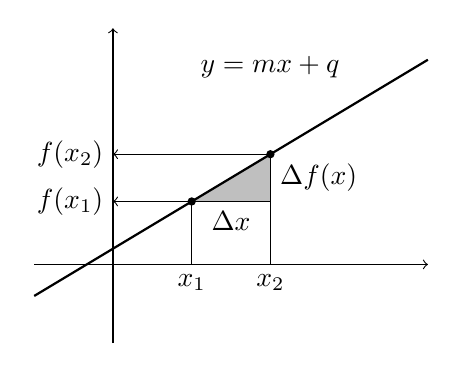
\begin{tikzpicture}[x=1.0cm,y=1.0cm]
    	\draw[->] (-1,0) -- (4,0);
      \draw[->] (0,-1) -- (0,3);
      % y = (3/5)*x + 1/5
      \fill[fill=lightgray,draw] (1,0.8) -- (2,0.8) node [midway,below]{$\Delta x$} -- (2,1.4) node [midway,right]{$\Delta f(x)$};
      \draw[thick] (-1,-0.4) -- (4,2.6);
      \draw[->] (1,0) node[below]{$x_1$} -- (1,0.8)
      -- (0,0.8) node[left]{$f(x_1)$};
      \draw[->] (2,0) node[below]{$x_2$} -- (2,1.4)
      -- (0,1.4) node[left]{$f(x_2)$};
      \fill (1,0.8) circle[radius=1.5pt];
      \fill (2,1.4) circle[radius=1.5pt];
      \node[left] at (3.0,2.5) {$y=mx+q$};
    \end{tikzpicture}
  \end{center}
  \caption{Il grafico di una funzione lineare.}
  \label{fig:funzione_lineare}
\end{figure}

Le \emph{funzioni lineari}%
\mymargin{funzione lineare}%
\index{funzioni lineari}
$f\colon \RR \to \RR$ sono le funzioni per le quali
esistono $m,q\in\RR$ tali che%
\footnote{%
Attenzione: nell'ambito dell'algebra lineare queste
funzioni verrebbero chiamate \emph{lineari affini}, mentre
le funzioni lineari dovrebbero sempre avere $q=0$.
Noi invece (come spesso accade nell'ambito dell'analisi)
chiameremo lineari queste funzioni e chiameremo
\emph{lineari omogenee} quelle con $q=0$.
Il termine \emph{lineare} pervade tutta la matematica 
e si applica in particolare alle equazioni che si ottengono 
tramite le funzioni lineari.
Purtroppo il nome scelto è fuorviante: la parola \emph{linea} viene 
usata a volte come abbreviazione di \emph{linea retta}, quando 
invece sarebbe più giusto utilizzare l'abbreviazione \emph{retta}
in quanto una linea può benissimo essere curva.
In altri contesti (come ad esempio nell'ambito degli ordinamenti)
il termine \emph{lineare} rappresenta un oggetto unidimensionale
senza ramificazioni ed è quindi maggiormente aderente 
al significato originale della parola.
} % marginnote
\[
  f(x) = mx + q.
\]

Se prendiamo due punti $(x_1,f(x_1))$
e $(x_2,f(x_2))$ sul grafico di una funzione lineare
possiamo osservare che si ha
\[
  \frac{f(x_2) - f(x_1)}{x_2 - x_1} = m.
\]
Il coefficiente $m$, dunque, rappresenta la pendenza del
grafico di $f$, ovvero il rapporto tra la variazione
dei valori della funzione $\Delta f = f(x_2) - f(x_1)$
e la variazione della variabile in ingresso
$\Delta x = x_2 - x_1$.
Geometricamente questo è il rapporto tra i due cateti
(base e altezza) che formano un triangolo rettangolo la
cui ipotenusa è il segmento che congiunge i due punti sul grafico.
Il fatto che questo rapporto sia costante significa,
in base al teorema di Talete, che i punti del grafico sono
allineati ovvero che il grafico di una funzione lineare è,
dal punto di vista geometrico, una retta.

\begin{definition}[retta]
  \index{retta}%
  \index{linea!retta}%
  Una \emph{linea retta} (più semplicemente: \emph{retta}) in è un sottospazio affine di dimensione 1 
  ovvero la traslazione di un sottospazio vettoriale di dimensione 1
  (si rimanda al corso di geometria).
\end{definition}

Tutte le rette del piano, 
tranne quelle parallele all'asse delle ordinate,
sono grafico di una funzione lineare.

Si osservi che per $m>0$ la funzione è strettamente crescente,
per $m=0$ la funzione è costante e per $m<0$ la funzione è
strettamente decrescente.

\section{funzioni quadratiche}
\label{sec:funzioni_quadratiche}

\begin{figure}
  \begin{center}
    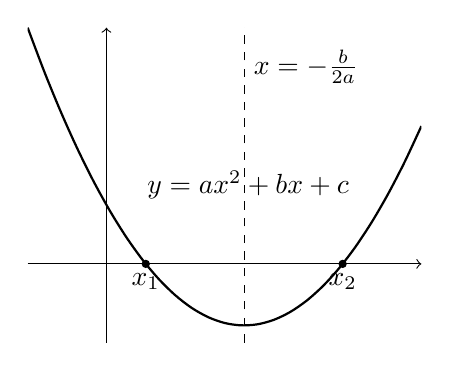
\begin{tikzpicture}[x=1.0cm,y=1.0cm]
      \clip(-1,-1) rectangle (4,3);
    	\draw[->] (-1,0) -- (4,0);
      \draw[->] (0,-1) -- (0,3);
      % y = (3/5)*x + 1/5
      \draw[dashed] (1.75,-1) -- (1.75,4);
      \node[right] at (1.75,2.5){$x=-\frac b {2a}$};
      \draw[domain=-1.0:4.0,smooth,variable=\x,thick] plot
      ({\x}, {0.5*(\x-0.5)*(\x-3.0)});
      \fill (0.5,0.0) node[below]{$x_1$} circle[radius=1.5pt];
      \fill (3,0.0) node[below]{$x_2$} circle[radius=1.5pt];
      \node at (1.8,1) {$y=ax^2+bx+c$};
    \end{tikzpicture}
  \end{center}
  \caption{Il grafico di una funzione quadratica.}
  \label{fig:funzione_quadratica}
\end{figure}

Le funzioni espresse mediante un \emph{polinomio di secondo grado}%
\mymargin{polinomio di secondo grado}%
\index{polinomio!di secondo grado}
\begin{equation}\label{eq:funzione_quadratica}
  f(x) = ax^2 + bx +c
\end{equation}
con $a,b,c\in \RR$, $a\neq 0$, si possono chiamare
\emph{funzioni quadratiche}%
\mymargin{funzioni quadratiche}%
\index{funzione!quadratica}.

Il modello di funzione quadratica è la funzione
$f(x) = x^2$ che (come tutte le potenze di esponente positivo e pari)
risulta essere una funzione pari, strettamente crescente
sull'intervallo $[0,+\infty)$ e strettamente decrescente
su $(-\infty,0]$. La funzione assume solamente valori non negativi
e si annulla solo per $x=0$.
Dunque l'equazione
\[
  x^2 = b
\]
non ha soluzione se $b<0$ ed ha come unica soluzione $x=0$ se $b=0$.
Se $b>0$ sappiamo che
questa equazione ha una unica soluzione positiva $x_1 = \sqrt{b}$
e, per simmetria, ha anche una soluzione negativa $x_2 = -\sqrt{b}$.
Sintetizzando si usa scrivere $x_{1,2} = \pm \sqrt{b}$
per unire in una unica riga le due definizioni.

La generica funzione quadratica~\eqref{eq:funzione_quadratica}
può essere ricondotta al caso modello tramite un cambio
di variabile lineare. In pratica si cerca di comporre il quadrato
di un binomio con un procedimento chiamato
\emph{completamento del quadrato}%
\mymargin{completamento del quadrato}%
\index{completamento del quadrato}:
\begin{equation}\label{eq:24589}
\begin{aligned}
f(x) = ax^2+bx+c
  &= a \Enclose{x^2+\frac b a x + \frac c a}\\
  &= a \Enclose{x^2+2 \frac{b}{2a} x + \frac{b^2}{4a^2} - \frac{b^2}{4a^2} + \frac c a}\\
  &= a \Enclose{\enclose{x+\frac{b}{2a}}^2 - \frac{b^2-4ac}{4a^2}} \\
  &= a\enclose{x+\frac b{2a}}^2  - \frac{b^2-4ac}{4a}.
\end{aligned}
\end{equation}

Ponendo $X=x+\frac b{2a}$ e $Y=y+\frac{b^2-4ac}{4a}$
l'equazione $y=ax^2+bx+c$ diventa quindi $Y=aX^2$. 
Significa
che il grafico della funzione quadratica~\eqref{eq:funzione_quadratica}
si ottiene traslando la curva $y = a x^2$ che, 
dal punto di vista geometrico, si può facilmente
dimostrare essere una parabola con fuoco
nel punto di coordinate $\enclose{0,\frac 1 {4a}}$
e asse la retta di equazione $x=0$.
Dunque il grafico di ogni funzione quadratica è una parabola, 
e più precisamente: ogni parabola con direttrice parallela all'asse delle
ascisse è il grafico di una funzione quadratica.

\begin{definition}[parabola]
  Una parabola con fuoco nel punto $\vec F=(F_1,F_2)\in \RR\times \RR$ 
  e retta direttrice 
  la retta $r \subset \RR\times\RR$ 
  è l'insieme dei punti  $\vec x = (x_1,x_2)\in \RR\times\RR$ 
  equidistanti da $\vec F$ e da $r$:
  \[
  \ENCLOSE{\vec x\in \RR\times\RR\colon 
  \sqrt{(x_1-F_1)^2 + (x_2-F_2)^2} 
  = \inf_{\vec P\in r}\sqrt{(x_1-P_1)^2+(y_1-P_1)^2}
  }.
  \]
\end{definition}

\begin{exercise}
  Si dimostri che per ogni $a\neq 0$ esiste $s\neq 0$ 
  per cui il riscalamento $X=sx$, $Y=sy$ porta il grafico della 
  parabola $y=ax^2$ nel grafico della parabola $Y=X^2$.
  Significa che a meno di isometrie e riscalamenti c'è una 
  unica parabola.
\end{exercise}

Ricordando le proprietà di monotonia della funzione $X\mapsto X^2$
possiamo dedurre che se $a>0$ la funzione $f(x)$ è strettamente
decrescente se ristretta all'intervallo 
$\left(-\infty,-\frac b {2a}\right]$ ed è invece strettamente crescente 
sull'intervallo $\left[-\frac b{2a},+\infty\right)$. 
Ha dunque un punto di minimo in $x=-\frac{b}{2a}$.
Inoltre (sempre se $a>0$) la funzione è superiormente illimitata.
Viceversa se $a<0$ la funzione è inferiormente illimitata ed ha 
un massimo nel punto $x=-\frac{b}{2a}$.

E' molto importante saper risolvere equazioni e disequazioni
quadratiche. Grazie a~\eqref{eq:24589} l'equazione
\[
 a x^2 + bx + c = 0
\]
risulta equivalente a
\[
  \enclose{x+\frac{b}{2a}}^2 = \frac{b^2-4ac}{4a^2}.
\]
Dunque se $b^2-4ac<0$ l'equazione $ax^2+bx+c=0$ non ha soluzioni.
Se $b^2-4ac=0$ l'equazione ha una unica soluzione $x=-\frac{b}{2a}$.
Infine se $b^2-4ac>0$ si ottiene
\[
  x+\frac b{2a} = \pm \frac{\sqrt{b^2-4ac}}{2a}
\]
da cui la famosa formula risolutiva
\mymark{***}
\begin{equation}\label{eq:secondo_grado}
  x_{1,2} = \frac{-b \pm \sqrt{b^2-4ac}}{2a}.
\end{equation}

Risolvendo le disequazioni allo stesso modo, si trova
che la funzione $ax^2+bx+c$ quando $a>0$ è positiva
nei punti esterni alle soluzioni dell'equazione
(in tutti i punti se le soluzioni non esistono) ed
è negativa nei punti interni alle due soluzioni.
Viceversa se $a<0$ la funzione è positiva all'interno
delle due soluzioni e negativa all'esterno.

\section{funzione esponenziale e potenza}
\label{sec:esponenziale}

Osserviamo che l'insieme $\RR_+ = \ENCLOSE{x\in \RR\colon x>0}$ 
dei reali positivi rispetto alla operazione di moltiplicazione 
risulta essere un gruppo moltiplicativo totalmente ordinato, 
denso e continuo. 
Abbiamo già dimostrato tutte queste proprietà della moltiplicazione.
La densità e continuità non vanno verificate in quanto sono proprietà 
dell'ordinamento e non dell'operazione, e l'ordinamento considerato 
su $\RR_+$ è quello ereditato da $\RR$.

Dunque fissato $a>0$ per il teorema~\ref{th:isomorfismo}
esiste una unica funzione $\exp_a\colon \RR \to \RR_+$ 
(chiamata \emph{funzione esponenziale}%
\mynote{funzione esponenziale}%
\index{funzione!esponenziale}%
\index{esponenziale}%
di base $a$)
che sia un omomorfismo monotono del gruppo additivo $\RR$ con il gruppo
moltiplicativo $\RR_+$ e tale che $\exp_a(1)=a$.
La proprietà di omomorfismo in questo caso 
si esprime nella forma seguente: 
\begin{equation}\label{eq:3589673}
  \exp_a(x+y) = \exp_a(x)\cdot \exp_a(y).
\end{equation}
Il teorema~\ref{th:isomorfismo}
ci dice anche che se $n\in \NN$ il valore $\exp_a(n)$ 
non è altro che il prodotto di $a$ 
con sé stesso $n$ volte: $\exp_a(n) = a^n$. 
Ha dunque senso definire 
$a^x = \exp_a(x)$ per ogni $x\in \RR$.
Avremo dunque la proprietà fondamentale della funzione 
esponenziale:
\[
  a^{x+y} = a^x\cdot a^y.
\]

Per ogni $a>0$ e $b\in \RR$ è dunque definita l'espressione $a^b$
(si legga: \emph{$a$ elevato alla potenza $b$}) che si chiama 
\emph{potenza}%
\mynote{potenza}%
\index{potenza}%
di base $a$ ed esponente $b$.

Quando l'esponente è negativo si ha 
\[
  a^{-x} = \frac{1}{a^x}  
\]
in quanto $a^x\cdot a^{-x} = a^{x-x} = a^0 = 1$.
In particolare $a^{-1} = \frac{1}{a}$ è un modo per denotare  
l'inverso moltiplicativo.

Se $a>1$ 
la funzione $a^x$ risulta essere strettamente crescente, 
se $a<1$ la funzione è strettamente decrescente 
e se $a=1$ la funzione $1^x=1$ è costante.

Se $a>0$ e $b>0$ vogliamo dimostrare che vale la proprietà:
\[
  (a\cdot b)^x = a^x\cdot b^x.
\]
Sarà sufficiente dimostrarlo per $a>1$ e $b>1$ in quanto gli 
altri casi si ottengono di conseguenza passando al reciproco.
Osservare che la funzione $f(x)=a^x\cdot b^x$ 
è un omomorfismo
\[
f(x+y) = a^{x+y}b^{x+y} = a^x a^y b^x b^y =  f(x)\cdot f(y)
\]
è crescente (in quanto prodotto di funzioni positive e crescenti)
e vale $f(1) = a\cdot b$. 
Dunque per l'unicità data dal teorema~\ref{th:isomorfismo}
possiamo affermare che $f(x)=(a\cdot b)^x$.

Infine possiamo dimostrare la proprietà delle potenze ripetute:
\[
  \enclose{a^b}^c = a^{b\cdot c}.
\]
Fissati $a>0$ e $b\in \RR$ consideriamo la funzione $f(x) = a^{b\cdot x}$.
osserviamo che $f(x+y) = a^{bx+by}=a^{bx}\cdot a^{by}$ dunque 
la funzione $f$ soddisfa la proprietà di additività. 
Inoltre è una funzione monotona perché composizione di funzioni monotone.
Infine $f(1) = a^b$ e dunque, per l'unicità data dal teorema~\ref{th:isomorfismo}
dovrà essere $f(x) = \enclose{a^b}^x$, come volevamo dimostrare. 

\begin{figure}
  \begin{center}
    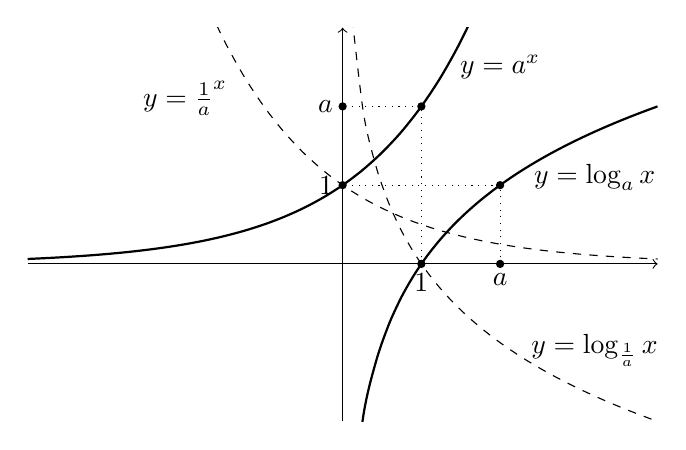
\begin{tikzpicture}[x=1.0cm,y=1.0cm]
      \clip(-4,-2) rectangle (4,3);
    	\draw[->] (-4,0) -- (4,0);
      \draw[->] (0,-2) -- (0,3);
      % y = (3/5)*x + 1/5
      \draw[dotted] (1,0) -- (1,2) -- (0,2);
      \draw[dotted] (2,0) -- (2,1) -- (0,1);
%      \node[right] at (1.75,2.5){$x=-\frac b {2a}$};
      \draw[domain=-2.0:4.0,smooth,variable=\x,dashed] plot
        ({\x}, {pow(2,-\x)});
      \draw[domain=0.1:4.0,smooth,variable=\x,dashed] plot
        ({\x}, {-ln(\x) / ln(2)});
      \draw[domain=-4.0:2.0,smooth,variable=\x,thick] plot
        ({\x}, {pow(2,\x)});
      \node at (2,2.5) {$y=a^x$};
      \node at (-2,2.1) {$y=\enclose{\frac 1 a}^x$};
      \fill (0,1.0) node[left]{\!\!$1$} circle[radius=1.5pt];
      \draw[domain=0.1:4.0,smooth,variable=\x,thick] plot
        ({\x}, {ln(\x) / ln(2)});
      \node at (3.2,1.1) {$y=\log_a x$};
      \node at (3.2,-1.1) {$y=\log_{\frac 1 a} x$};
      \fill (1,0) node[below]{$1$} circle[radius=1.5pt];
      \fill (0,2) node[left]{$a$} circle[radius=1.5pt];
      \fill (2,0) node[below]{$a$} circle[radius=1.5pt];
      \fill (2,1) circle[radius=1.5pt];
      \fill (1,2) circle[radius=1.5pt];
    \end{tikzpicture}
  \end{center}
  \caption{Il grafico della funzione esponenziale e logaritmo 
  in base $a>1$ e $\frac 1 a < 1$ ($a=2$ in figura).}
  \label{fig:esponenziale_logaritmo}
\end{figure}
%
\begin{figure}
  \begin{center}
    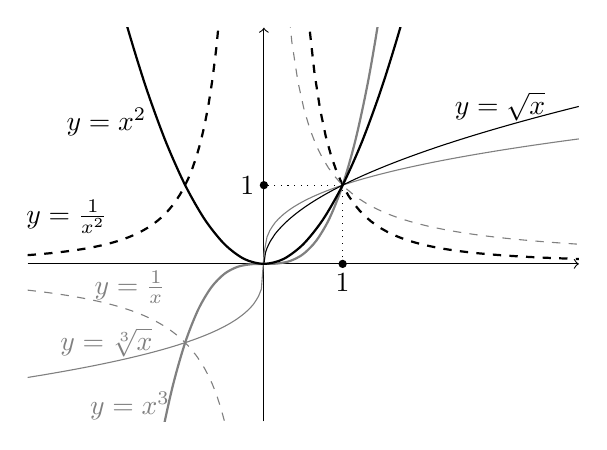
\begin{tikzpicture}[x=1.0cm,y=1.0cm]
      \clip(-3,-2) rectangle (4,3);
    	\draw[->] (-3,0) -- (4,0);
      \draw[->] (0,-2) -- (0,3);
      \draw[dotted] (1,0) -- (1,1) -- (0,1);
      % \draw[dotted] (2,0) -- (2,1) -- (0,1);
      \draw[domain=0.5:4,samples=50,variable=\x,thick,dashed] plot
        ({\x}, {1/(\x*\x))});
      \draw[domain=-3:-0.5,samples=50,variable=\x,thick,dashed] plot
        ({\x}, {1/(\x*\x))});
      \draw[domain=0.2:4,samples=50,variable=\x,dashed,color=gray] plot
        ({\x}, {1/(\x))});
      \draw[domain=-3:-0.5,samples=50,variable=\x,dashed,color=gray] plot
        ({\x}, {1/(\x))});
      \draw[domain=-2.0:2.0,smooth,variable=\x,thick,color=gray] plot
        ({\x}, {\x*\x*\x)});
      \draw[domain=-3.1:4.0,samples=200,variable=\x,color=gray] plot
        ({\x}, {pow(abs(\x),1/3)*\x / abs(\x)});
      \draw[domain=-3.0:3.0,smooth,variable=\x,thick] plot
        ({\x}, {\x*\x});
      \draw[domain=0.0:4.0,samples=200,variable=\x] plot
      ({\x}, {pow(\x,1/2)});
      \node at (-2.0,1.8) {$y=x^2$};
      \node at (3,2) {$y=\sqrt{x}$};
      \node[color=gray] at (-1.7,-1.8) {$y=x^{3}$};
      \node[color=gray] at (-2.0,-1) {$y=\sqrt[3]{x}$};
      \node[color=gray] at (-1.7,-0.3) {$y=\frac 1 x$};
      \node at (-2.5,0.6) {$y=\frac 1 {x^2}$};
      \fill (1,0) node[below]{$1$} circle[radius=1.5pt];
      \fill (0,1) node[left]{$1$} circle[radius=1.5pt];
    \end{tikzpicture}
  \end{center}
  \caption{Grafici tipici di potenze e radici.}
  \label{fig:potenza_radice}
\end{figure}

Osserviamo che la funzione potenza $x^\alpha$ (dove si tiene fisso 
l'esponente e si fa variare la base) è definita tramite la funzione esponenziale 
per ogni $x>0$ e per ogni $\alpha\in \RR$.
Se $\alpha>0$ è naturale definire $0^\alpha = 0$ e quindi 
se $\alpha>0$ 
possiamo considerare definito $x^\alpha$ per ogni $x\ge 0$.
Verifichiamo che la funzione $f(x)=x^\alpha$ è strettamente crescente
 se $\alpha>0$. 
Infatti se $x_2>x_1>0$ e se $\alpha>0$ si ha 
\[
  x_2^\alpha 
  = \enclose{\frac {x_2} {x_1}}^\alpha\cdot {x_1}^\alpha 
  > \enclose{\frac {x_2} {x_1}}^0 \cdot {x_1}^\alpha 
  = x_1^\alpha.
\]


\section{radice $n$-esima}

Dalle proprietà delle potenze ripetute deduciamo che se $x>0$
e $n\in\NN$, $n\ge 1$, si ha $(x^n)^\frac 1 n = x$.
Significa che $x^{\frac 1 n}$ è la funzione inversa di $x^n$ per $x>0$.
Ma la funzione $x^n$ è definita anche per $x\le 0$ e si distinguono due 
casi qualitativamente diversi in base alla parità di $n$.

Se $n$ è pari la funzione $x\mapsto x^n$ non è invertibile in quanto 
$(-x)^n = x^n$. 
Se però restringiamo la funzione $x^n$ ai numeri reali non negativi
la funzione risulta invertibile e la funzione inversa 
che si denota con $x\mapsto\sqrt[n]{x}$ 
può essere definita mediante le potenze come segue:
\[
   \sqrt[n]{x} = \begin{cases}
      x^{\frac 1 n} & \text{se $x>0$}\\
      0 & \text{se $x=0$}
   \end{cases} \qquad \text{se $n$ è pari}.
\]
Se $n$ è dispari la funzione $x\mapsto x^n$ è invertibile su tutto 
$\RR$. 
Infatti $(-x)^n = -x^n$ dunque tale funzione mantiene il segno 
del suo argomento. In tal caso la funzione inversa 
denotata con $x\mapsto \sqrt[n]{x}$
è anch'essa definita su tutto $\RR$ e può essere definita 
nel modo seguente
\[
   \sqrt[n]{x} = \begin{cases}
      x^{\frac 1 n} & \text{se $x>0$} \\ 
      0 & \text{se $x=0$}\\
      -(-x)^{\frac 1 n} & \text{se $x<0$}
   \end{cases}
   \qquad\text{se $n$ è dispari}
\]

Quando l'argomento è positivo la radice $n$-esima 
potrebbe anche essere definita utilizzando il teorema~\ref{th:divisibile}
di divisibilità nell'ambito del gruppo moltiplicativo $\RR_+$.

La radice seconda $\sqrt[2]{x}$ viene usualmente chiamata 
\emph{radice quadrata}%
\mynote{radice quadrata}%
\index{radice!quadrata} e
viene denotata con il simbolo $\sqrt{x}$.
Analogamente la radice terza $\sqrt[3]{x}$ viene usualmente chiamata 
\emph{radice cubica}%
\mynote{radice cubica}%
\index{radice!cubica}.

Per come è definita la radice $n$-esima si ha 
\[
  \sqrt[n]{x^n} = 
  \begin{cases}
     \abs{x} & \text{se $n$ è pari,} \\
     x & \text{se $n$ è dispari.}
  \end{cases}
\]
E' facile verificare che le proprietà 
$\sqrt[n]{x\cdot y} = \sqrt[n]{x} \cdot \sqrt[n]{y}$
e $\sqrt[n]{\sqrt[m]{x}} = \sqrt[nm]{x}$
sono valide in tutti i casi in cui ambo i membri sono ben definiti. 

Ricordiamo che in base al teorema~\ref{th:pitagora} sappiamo 
che $\sqrt 2$ è irrazionale 
(non è razionale, ovvero non è elemento di $\QQ$)
in quanto risolve l'equazione $x^2=2$.

Possiamo quindi osservare che $\QQ$, come $\RR$, è un campo totalmente 
ordinato.
Evidentemente $\QQ$ non può essere continuo, perché se lo fosse 
dovrebbe essere uguale ad $\RR$ per il teorema di unicità degli 
isomorfismi dei gruppi continui ordinati e dovrebbe quindi 
contenere il numero $\sqrt 2$. 

\section{logaritmo}
%
Se $a>0$, $a\neq 1$ la funzione esponenziale 
$\exp_a\colon \RR \to \RR_+$ è bigettiva. 
La funzione inversa $\log_a\colon \RR_+\to \RR$ si chiama \emph{logaritmo}%
\mynote{logaritmo}%
\index{logaritmo} in base $a$ 
e si caratterizza con la seguente proprietà:
\[
  \log_a x = y \iff a^y = x.
\]
La proprietà di omomorfismo diventa:
\[
  \log_a(x\cdot y) =  \log_a x + \log_a y.
\]
Ovviamente vale $\log_a a = 1$ e $\log_a 1 = 0$.
Se $a>1$ la funzione logaritmo è strettamente crescente, se $a<1$ è strettamente decrescente.
La proprietà dell'esponenziale ripetuto si traduce nella seguente:
\[
  \log_a (x^y) = y \log_a x.
\]
E' anche piuttosto utile ricordare la formula per il cambiamento di base:
\[
\log_a x = \frac{\log_b x}{\log_a b}
\]
(valida, come tutte le formule enunciate, se l'argomento del logaritmo 
è positivo e se le basi sono positive diverse da $1$ e diverse tra loro).
Quest'ultima formula si dimostra moltiplicando ambo i membri per $\log_a b$ 
e prendendo quindi l'esponenziale con base $b$ di ambo i membri.


\section{equazioni e disequazioni}

Un problema matematico molto comune è quello di dover risolvere 
equazioni e disequazioni del tipo:
\begin{equation}\label{eq:573197}
  f(x) = b, \quad f(x) \ge b, \quad f(x) > b, 
  \quad f(x) \le b, \quad f(x) < b
\end{equation}
dove $f\colon A \subset \RR \to\RR$ è una funzione data e 
$b\in \RR$ è fissato.

Quando $f$ è strettamente crescente e $b\in f(A)$ 
la soluzione può essere 
scritta banalmente: 
ovviamente deve essere $x\in A$
e ogni equazione o disequazione in~\eqref{eq:573197}
avrà la corrispondente soluzione:
\[
  x= f^{-1}(b), \quad x \ge f^{-1}(b), \quad x>f^{-1}(b),
  \quad x \le f^{-1}(b), \quad x < f^{-1}(b).
\]
Se la funzione fosse strettamente decrescente 
si può procedere allo stesso modo, ma le disuguaglianze si invertono.
Se la funzione fosse strettamente crescente su alcuni intervalli 
e strettamente decrescente su altri si potranno separare i diversi 
casi e si otterranno più soluzioni espresse da uguaglianze
o disuguaglianze.

\begin{example}
  Si risolva la disequazione 
  \[
   \log_2\Enclose{\sqrt[3]{(x+1)^4-3}-2} \le 3. 
  \]
\end{example}%
\begin{proof}[Svolgimento.]
La funzione logaritmo è strettamente crescente ed è definita 
quando l'argomento è positivo. 
Dunque la disequazione data 
è equivalente al sistema di disequazioni:
\[
0 < \sqrt[3]{(x+1)^4 - 3} - 2 \le 8.  
\]
Possiamo sommare $2$ per ottenere 
\[
  2 < \sqrt[3]{(x+1)^4 - 3} \le 10.  
\]
La funzione radice cubica è strettamente crescente 
su tutto $\RR$ quindi possiamo invertirla elevando 
tutto al cubo:
\[
 8 < (x+1)^4 - 3 \le 1000.
\]
Sommiamo $3$:
\[
11 < (x+1)^4 \le 1003.  
\]
L'elevamento alla quarta potenza è strettamente crescente 
solo quando l'argomento è positivo, ed è una funzione pari.
Possiamo quindi affermare che le nostre disequazioni sono 
equivalenti all'unione delle soluzioni di due sistemi:
\[
  \sqrt[4]{11} < x+1 \le \sqrt[4]{1003}
  \qquad\text{o}\qquad 
  -\sqrt[4]{1003} \le x+1 < \sqrt[4]{11}.
\]
Sottraendo $1$ otteniamo infine 
\[
  \sqrt[4]{11} -1 < x \le \sqrt[4]{1003} - 1
  \qquad\text{o}\qquad 
  -\sqrt[4]{1003} -1 \le x < \sqrt[4]{11} -1.
\]
In definitiva l'insieme delle soluzioni è 
\[
\left[-\sqrt[4]{1003} - 1, \sqrt[4]{11}-1\right)
\cup \left(\sqrt[4]{11}-1 , \sqrt[4]{1003} -1\right].  
\]
\end{proof}

Nell'esempio precedente la funzione 
$f(x) = \log_2\Enclose{\sqrt[3]{(x+1)^4-3}-2}$
è ottenuta mediante composizione di funzioni elementari:
\begin{align*}
f &= (x\mapsto \log_2 x)\circ(x\mapsto x-2)\circ (x \mapsto \sqrt[3]{x})\\
  &\quad \circ (x \mapsto x-3) \circ (x\mapsto x^4) \circ (x\mapsto x+1).
\end{align*}
Negli intervalli in cui tutte queste funzioni sono invertibili 
la funzione inversa si ottiene componendo, in ordine opposto,
tutte le inverse:
\begin{align*}
  f^{-1} &= (x\mapsto x-1) \circ (x\mapsto \sqrt[4]{x}) \circ (x \mapsto x+3) \\
    &\quad \circ (x \mapsto x^3) \circ (x \mapsto x+2) \circ (x\mapsto 2^x).
\end{align*}
In effetti il caposaldo $\sqrt[4]{1003}-1$ è proprio tale 
funzione valutata in $b=3$.

Il metodo precedente è puramente algebrico e 
si applica alle equazioni 
come la~\eqref{eq:573197} dove la variabile $x$ 
compare una sola volta e dove la funzione $f$ si esprime 
come composizione di funzioni elementari di cui sappiamo 
scrivere la funzione inversa. 

Ben diverso è il caso in cui nell'equazione la variabile $x$ 
compare più di una volta.
In alcuni casi, come ad esempio,
\[
  x^2 > 2x - 1  
\]
queste equazioni 
possono essere ricondotte al caso precedente tramite 
opportune manipolazioni algebriche.
Il caso delle equazioni quadratiche lo abbiamo 
fatto nel paragrafo precedente utilizzato il completamento 
del quadrato: $x^2-2x = (x-1)^2-1$. 
In altri casi, come ad esempio l'equazione
\[
  2^x = x^2
\]  
le manipolazioni algebriche non sono utili.
Nel capitolo sul calcolo differenziale svilupperemo degli strumenti 
che ci permetteranno di determinare l'andamento di molte di queste 
di funzioni. 
Nel capitolo sulle successioni svilupperemo invece gli strumenti 
che ci permetteranno di determinare le soluzioni mediante 
algoritmi di approssimazione.
Questi strumenti presuppongono il concetto 
di limite e continuità: è sostanzialmente questo che identifica 
la materia chiamata analisi matematica.

\section{cardinalità infinite}

Abbiamo già osservato che $\NN$ è un insieme infinito e dunque (per il teorema~\ref{th:cantor_bernstein})
anche $\ZZ$, $\QQ$ e $\RR$ sono infiniti.
Per gli insiemi finiti se $A\subset B$ ma $A\neq B$ risulta $\#A < \# B$
in quanto $\#A - \#B = \#(B\setminus A) > 0$. 
Dobbiamo però osservare che lo stesso non vale per gli insiemi infiniti.
In effetti la funzione $s\colon \NN \to \NN$ definita da $s(x)=x+1$
risulta essere una bigezione tra $\NN$ e $\NN\setminus\ENCLOSE{0}$. 
Dunque $\#\NN = \#(\NN\setminus\ENCLOSE{0})$ 
nonostante la differenza tra i due insiemi $\ENCLOSE{0}$ abbia 
cardinalità $1$. 
Anche l'insieme dei numeri pari o l'insieme 
dei quadrati perfetti (come aveva notato già Galileo)
hanno la stessa cardinalità di $\NN$ in quanto le funzioni $n\mapsto 2n$
e la funzione $n\mapsto n^2$ sono iniettive.

Non è difficile trovare una funzione iniettiva da $\ZZ$ in $\NN$
(lo lasciamo per esercizio): questo dimostra che anche $\#\ZZ = \# \NN$

Cantor dimostra addirittura che $\#\QQ = \NN$: per farlo utilizza il seguente.

\begin{theorem}[primo metodo diagonale di Cantor]
\label{th:Cantor_primo}%
\index{Cantor!primo metodo diagonale}%
L'insieme $\NN \times \NN$ ha la stessa cardinalità di $\NN$. Di conseguenza
\[
  \# \NN = \# \ZZ = \# \QQ.
  \]
\end{theorem}
%
\begin{proof}[Idea di dimostrazione]
  Numerare le caselle di una scacchiera infinita
  come in Figura~\ref{fig:cantor1}.
  
  Visto che è piuttosto facile trovare una funzione iniettiva 
  da $\QQ$ in $\NN \times \ZZ$ si deduce facilmente che $\#\QQ = \#\NN$.
\end{proof}

\begin{figure}
  \begin{tabular}{c|ccccccc}
   $m$ & $\ddots$\\
   $\vdots$ & $\ddots$ & $\ddots$\\
   3 & 9 & $\nwarrow$ & $\ddots$ \\
   2 & 5 & 8 & 12 & $\ddots$ \\
   1 & 2 & 4 & 7 & 11 & $\ddots$ \\
   0 & 0 & 1 & 3 & 6 & 10 & $\ddots$ \\ \hline
     & 0 & 1 & 2 & 3 & 4 & $\dots$ & $n$
  \end{tabular}
  \caption{
    La numerazione diagonale delle caselle
    di una scacchiera infinita. Si potrebbe verificare
    che il numero presente nella casella di coordinate $(n,m)$
    si scrive come $f(n,m) = \frac{(n+m+1)(n+m)}{2}+m$
    ed è una funzione bigettiva $f\colon \NN\times\NN \to\NN$.}
  \label{fig:cantor1}
\end{figure}

A questo punto si potrebbe pensare che
tutti gli insiemi infiniti siano numerabili.
Invece preso un qualunque insieme (anche infinito)
esiste un insieme con cardinalità strettamente maggiore
come dimostrato nel seguente teorema che è un piccolo gioiello della logica.
In effetti il metodo utilizzato è assimilabile al paradosso del mentitore 
ed è la stessa idea usata nel paradosso di Russell (teorema~\ref{th:Russell}).
L'insieme delle parti $\mathcal P(A)$ è definito a pag.~\pageref{def:insieme_parti}.
%
\begin{theorem}[Cantor]%
\label{th:Cantor}%
  Se $A$ è un qualunque insieme allora $\# \mathcal P(A) > \# A$.
\end{theorem}
%
\begin{proof}
  E' chiaro che $\# A \le \#\mathcal P(A)$ in quanto 
  la funzione $f\colon A \to \mathcal P(A)$ definita da $f(x)=\ENCLOSE{x}$
  è ovviamente iniettiva.

  Supponiamo allora per assurdo che esista $f\colon A\to \mathcal P(A)$
  bigettiva e consideriamo l'insieme 
  \[
    C = \ENCLOSE{x\in A \colon x\not\in f(x)}.  
  \]
  Se $f$ fosse surgettiva dovrebbe esistere $c\in A$ tale che $f(c) = C$.
  Possiamo allora chiederci se $c\in C$ e scoprire che, 
  per definizione di $C$ la proposizione $c\in C$ è equivalente 
  a $c\not\in f(c) = C$. 
  Dunque $c\in C \iff c\not\in C$, che è assurdo.
\end{proof}
%
\begin{corollary}[non esiste l'insieme di tutti gli insiemi]
  Se esistesse un insieme $\mathcal U$ (universo) 
  tale che $\forall x\colon x \in U$, allora 
  si avrebbe $\mathcal \P(\mathcal U) \subset \mathcal U$
  contraddicendo il teorema precedente.
\end{corollary}
%
Per quanto riguarda l'insieme $\RR$ si
scopre in effetti che $\#\RR > \#\NN$
(sempre grazie a Cantor, teorema~\ref{th:cantor_secondo})
e si potrebbe dimostrare che effettivamente $\#\RR = \#\mathcal P(\NN)$.

\section{i numeri complessi}

Dal punto di vista geometrico l'insieme $\CC$ dei \emph{numeri complessi}%
\mymargin{numeri complessi}%
\index{numeri!complessi}
\index{$\CC$}
può essere visto come un modello del piano euclideo.
Sul piano euclideo fissiamo arbitrarimente un punto $0$ in modo da ottenere uno spazio
vettoriale e fissiamo, arbitrariamente, una base $e_1$, $e_2$.
Identifichiamo ogni punto del piano con i corrispondenti vettori
applicati in $0$. La retta generata dal vettore $e_1$ la identifichiamo
con la retta $\RR$ dei numeri reali e quindi poniamo $1=e_1$.
La retta ortogonale generata dal vettore $e_2$ verrà chiamata
retta dei \emph{numeri immaginari} e definiamo $i=e_2$.

Un generico punto $z$ del piano $\CC$ potrà essere scritto in
maniera univoca nella base scelta: $z = x e_1 + y e_2$ ovvero,
per come abbiamo chiamato $e_1$ ed $e_2$:
\[
z = x + i y.
\]
Tale $z$ viene chiamato
\emph{numero complesso} con parte reale $x$ e parte immaginaria $y$.
Questa rappresentazione del numero complesso $z$ viene
chiamata \emph{rappresentazione cartesiana}%
\mymargin{rappresentazione cartesiana}%
\index{rappresentazione!cartesiana} in quanto definisce
il punto $z$ del piano complesso tramite le sue coordinate cartesiane
$x$ e $y$.
I numeri reali sono \emph{immersi} nei complessi, nel senso che se
$x\in \RR$ allora $z= x + i\cdot 0 = x$ è anche un numero complesso.
Il numero complesso $i = 0 + i\cdot 1$ viene chiamata \emph{unità immaginaria}%
\mymargin{unità immaginaria}%
\index{unità!immaginaria}
e i numeri complessi della forma $iy$ sono chiamati \emph{immaginari}.
\index{numeri!immaginari}
\index{immaginario}
Un numero
complesso $z = x+iy$ è quindi una somma tra un numero reale ed un numero
immaginario. Il numero reale $x$ viene chiamato \emph{parte reale}
\index{parte!reale}
di $z$ e
si denota con $x=\Re z$.
\mymargin{$\Re z$}%
\index{$\Re z$}
Il numero reale $y$ viene chiamato
\emph{parte immaginaria}
\index{parte!immaginaria}
di $z$ e si denota con $y=\Im z$
\mymargin{$\Im z$}%
\index{$\Im z$}
(osserviamo che la parte immaginaria di un numero complesso è un numero
reale, non immaginario). Dunque $z= \Re z + i \Im z$.

L'insieme $\CC$, per come
è stato costruito, è uno spazio vettoriale reale di dimensione $2$.
Abbiamo quindi già definite la \emph{addizione}%
\mymargin{addizione}%
\index{addizione}
\index{complessi!addizione}
tra elementi di $\CC$ e la moltiplicazione
tra elementi di $\CC$ ed elementi di $\RR$,
se $a,b,c,d,t\in \RR$ si ha:
\begin{gather*}
 (a+ib) + (c+id) = (a+c) + i (b+d), \\
 t(a+ib) = ta + itb.
\end{gather*}

Vogliamo estendere la \emph{moltiplicazione}%
\mymargin{moltiplicazione}%
\index{moltiplicazione} a tutte le coppie di numeri complessi.
\index{complessi!moltiplicazione}
Imponendo (arbitrariamente) che valga $i\cdot i = -1$ e che rimanga
valida la proprietà distributiva, si ottiene
questa definizione:
\[
   (a+ib) \cdot (c+id) = (ac-bd) + i(ad+bc).
\]

Si può verificare che questa moltiplicazione estende quella ``scalare'' definita
in precedenza.
E' anche facile verificare che addizione e moltiplicazione soddisfano
le proprietà commutativa associativa e distributiva,
che $0$ è elemento neutro per la addizione, che $1$ è elemento neutro
della moltiplicazione.
Si osservi che se $z=x+iy$ non è nullo, allora
\[
  (x+iy) \cdot \frac{x-iy}{x^2+y^2} = 1.
\]
Significa che ogni $z\neq 0$ ammette inverso moltiplicativo e quindi $\CC$
risulta essere un campo.

Osserviamo che su $\CC$ non si definisce una relazione d'ordine perché
in effetti non è possibile definire un ordine ``compatibile'' con le operazioni
appena definite.%
\footnote{%
Se $\CC$ fosse un campo ordinato per assurdo
si dovrebbe avere,
che $z^2\ge 0$ per ogni $z\in \CC$ (questo è vero in tutti i campi ordinati). 
Ma
allora $-1 =i^2 \ge 0$ cioè $1\le 0$ che è in contraddizione
con la proprietà $0<1$ valida in ogni campo ordinato.
} % marginnote

Su $\CC$ definiamo delle ulteriori operazioni.
Il \emph{coniugato}%
\mymargin{coniugato}%
\index{coniugato}%
\index{complessi!coniugio}
di un numero complesso $z=x+iy$ è il numero
$\bar z = x - iy$. Geometricamente l'operazione di coniugio è una simmetria
rispetto alla retta reale. I numeri reali sono in effetti punti fissi del
coniugio (il coniugato di un numero reale è il numero stesso).
E' un semplice esercizio verificare che il coniugio ``attraversa''
somma e prodotto:
\[
\overline{z+w} = \bar z + \bar w, \qquad
\overline{z\cdot w} = \bar z \cdot \bar w.
\]
Ovviamente risulta $\overline {\bar z} = z$.
E' anche utile osservare che si ha:
\begin{equation}\label{eq:re_im}
  \Re z = \frac{z+\bar z}{2}, \qquad
  \Im z = \frac{z-\bar z}{2i}
\end{equation}
e
\[
z \cdot \bar z = (x+iy)(x-iy) = x^2-i^2y^2 = x^2+y^2.
\]

Possiamo allora definire il
\emph{modulo}%
\mymargin{modulo}%
\index{modulo}%
\index{complessi!modulo}
 di un numero complesso $z=x+iy$
come il numero reale
\[
\abs{z} = \sqrt{z\cdot\bar z} = \sqrt{x^2+y^2}.
\]
Geometricamente tale quantità rappresenta la distanza del punto $z$
dal punto $0$ e quindi la distanza tra due numeri complessi $z$ e
$w$ si potrà rappresentare con $\abs{z-w}$.

Osserviamo che se $z = x \in \RR \subset \CC$ il modulo di $z$ coincide
con il valore assoluto: $\abs{z} = \sqrt{x^2} = \abs{x}$ e per questo
motivo non distinguiamo, nelle notazioni, il modulo dal valore assoluto.
Più in generale risulta per ogni $z\in \CC$ (la verifica è immediata):
\[
  \abs{\Re z} \le \abs{z}, \qquad
  \abs{\Im z} \le \abs{z}.
\]

Possiamo a questo punto trovare una utile formula per calcolare
il reciproco di un numero complesso. Essendo infatti
$z\cdot \bar z = \abs{z}^2$ si osserva che
\[
  \frac{1}{z}
  = \frac{\bar z}{ \bar z \cdot z}
  = \frac{\bar z}{\abs{z}^2}.
\]

\begin{theorem}
Il modulo di un numero complesso soddisfa (come il valore assoluto)
le seguenti proprietà
\begin{enumerate}
\item $\big\lvert\abs{z}\big\rvert = \abs{z}$,
\item $\abs{-z} = \abs{z}$ = $\abs{\bar z}$,
\item $\abs{z\cdot w} = \abs{z}\cdot\abs{w}$.
\item $\abs{z+w} \le \abs{z}+\abs{w}$ (convessità),
\item $\abs{z-w} \le \abs{z-v} + \abs{v-w}$ (disuguaglianza triangolare),
\end{enumerate}
\end{theorem}
%
\begin{proof}
La prima proprietà è ovvia in quanto il valore assoluto di un numero reale
non negativo è il numero stesso.

La seconda proprietà viene immediatamente dalla definizione.

Per la terza proprietà sia $z=x+iy$, $w=a+ib$.
Allora:
\begin{align*}
\abs{z\cdot w}
&= \abs{(x+iy)\cdot(a+ib)}
=\abs{xa - y b+ i(xb + ay)} \\
&= \sqrt{(xa-yb)^2 + (xb+ay)^2}\\
&=\sqrt{x^2 a^2 + y^2b^2 - 2xayb + x^2b^2+a^2y^2+2xbay} \\
&=\sqrt{x^2 a^2 + y^2 b^2 + x^2 b^2 + a^2 y^2}\\
&=\sqrt{x^2(a^2+b^2) + y^2(a^2+b^2)}\\
&=\sqrt{(x^2+y^2)(a^2+b^2)}
=\abs{x+iy} \cdot \abs{a+ib}\\
&=\abs{z}\cdot\abs{w}.
\end{align*}

Per la quarta disuguaglianza osserviamo che si ha
\[
  \abs{z+w}^2 = (z+w)\cdot(\bar z + \bar w)
  = \abs{z}^2 + \abs{w}^2 + z\cdot \bar w + \bar z \cdot w
\]
e visto che
\[
  z\cdot \bar w + \bar z \cdot w
  = z \cdot \bar w + \overline{z \cdot \bar w}
  = 2 \Re(z\bar w)
  \le 2 \abs {z\bar w}
  = 2 \abs{z}\cdot\abs{\bar w}
  = 2 \abs{z}\cdot\abs{w}
\]
otteniamo
\[
 \abs{z+w}^2 \le \abs{z}^2+\abs{w}^2 + 2 \abs{z}\cdot\abs{w}
 =\enclose{\abs z + \abs w}^2
\]
che è equivalente alla disuguaglianza di convessità.

La disuguaglianza triangolare è conseguenza immediata della convessità, infatti
\[
  \abs{z-w} = \abs{(z-v) + (v-w)}
  \le \abs{z-v} + \abs{v-w}.
\]
\end{proof}

\begin{figure}
  \begin{center}
    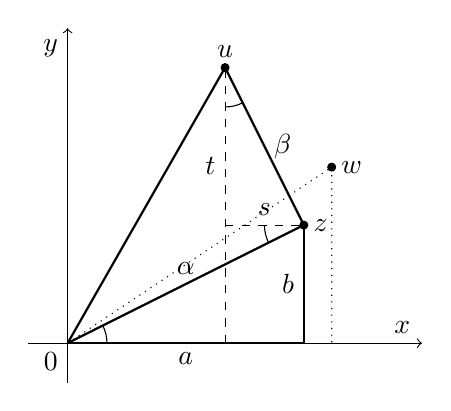
\begin{tikzpicture}[x=0.5cm,y=0.5cm]
    	\draw[->] (-1,0) -- (9,0);
      \draw[->] (0,-1) -- (0,8);
      %
      \draw[dotted] (0,0) -- ({sqrt(45)},{sqrt(20)}) -- ({sqrt(45)},0);
      \draw[fill] ({sqrt(45)},{sqrt(20)}) node[right] {$w$} circle [radius=0.1];
      %
      \draw[thick] (0,0) -- (6,0);
      \draw[thick] (0,0) -- (6,3);
      \draw[thick] (0,0) -- (4,7);
      \draw[thick] (6,0) -- (6,3);
      \draw[thick] (6,3) -- (4,7);
      %
      \draw[dashed] (4,0) -- (4,7);
      \draw[dashed] (4,3) -- (6,3);
      %
      \draw (1,0) arc (0:{atan(1/2)}:1);
      \draw (6,3)+(-1,0) arc (180:{180+atan(1/2)}:1);
      \draw (4,7)+(0,-1) arc (-90:{-90+atan(1/2)}:1);
      %
      \draw[fill] (6,3) node[right] {$z$} circle [radius=0.1];
      \draw[fill] (4,7) node[above] {$u$} circle [radius=0.1];
      %
      \node[below] at (3,0) {$a$};
      \node[left] at (6,1.5) {$b$};
      \node[above] at (3,1.5) {$\alpha$};
      \node[right] at (5,5) {$\beta$};
      \node[above] at (5,3) {$s$};
      \node[left] at (4,4.5) {$t$};
      \node[above] at (8.5,0) {$x$};
      \node[left] at (0,7.5) {$y$};
      \node[below left] at (0,0) {$0$};
    \end{tikzpicture}
  \end{center}
  \caption{Consideriamo i numeri complessi $z=a+ib$ e $w=\alpha+i\beta$
  e supponiamo che sia $\alpha^2 = a^2+b^2$.
  Si consideri il punto $u$ che si ottiene ruotando il punto $w$ dell'angolo
  individuato dal punto $z$. Si avrà allora $u=a-s + i(b+t)$ dove $s$ e $t$
  sono i cateti del triangolo rettangolo con ipotenusa $\beta$.
  Grazie alle proprietà di similitudine dei triangoli si ha
  $\frac{s}{\beta} = \frac{b}{\alpha}$ e $\frac{t}{\beta} = \frac{a}{\alpha}$
  da cui si ottiene quindi $u = a-\frac{b\beta}{\alpha}+i(b+\frac{a\beta}{\alpha})$
  ovvero $\alpha u = (a\alpha - b \beta) + i (b\alpha + a \beta) = z\cdot w$.
  Significa che il numero complesso $z\cdot w$ si trova sulla semiretta
  che individua un angolo che è la somma degli angoli individuati
  dai numeri complessi $z$ e $w$.
  }
  \label{fig:prodotto_complesso}
\end{figure}

Possiamo ora dare una interpretazione geometrica del prodotto $z\cdot w$
tra due numeri complessi. In primo luogo sappiamo che $\abs{z\cdot w} = \abs{z} \cdot \abs{w}$ e dunque il punto del piano che rappresenta il prodotto $z\cdot w$ si trova ad una distanza dall'origine che è pari al prodotto delle distanze
dei punti $z$ e $w$. Inoltre l'angolo individuato da $z\cdot w$ rispetto
all'asse delle $x$ positive risulta uguale alla somma
degli angoli individuati dai punti $z$ e $w$ come mostrato in figura~\ref{fig:prodotto_complesso}.

Anche il piano dei numeri complessi può essere esteso aggiungendoci
un punto all'\emph{infinito}%
\mymargin{infinito}%
\index{infinito}.
A differenza dei reali, su cui era presente un ordinamento che era utile conservare,
nel caso dei numeri complessi è più usuale utilizzare un unico punto infinito
che si denota con \emph{$\infty$}%
\mymargin{$\infty$}%
\index{$\infty$}.
Definiamo il piano dei complessi estesi $\bar \CC$ come
\[
\bar \CC = \CC \cup \ENCLOSE{\infty}.
\]
Definiamo
\begin{align*}
  z + \infty &= \infty \qquad \forall z \in \CC\\
  z - \infty &= \infty \qquad \forall z \in \CC\\
   z\cdot \infty &= \infty \qquad \forall z \in \bar\CC\setminus\ENCLOSE{0} \\
   z / \infty &= 0 \qquad \forall z \in \CC \\
   z / 0 &= \infty \qquad \forall z \in \bar \CC \setminus\ENCLOSE{0}\\
   \bar \infty &= \infty \\
   \abs{\infty} &= +\infty \in \bar \RR.
\end{align*}
Si noti che abbiamo definito la divisione per zero di numeri complessi
(e quindi anche reali) diversi da zero. Il risultato è $\infty$ e quindi
rimane confermato che la divisione per zero non è una operazione valida
se vogliamo un risultato finito.
Una quantità $z\in \bar \CC$ sarà detta \emph{finita} se $z\in \CC$.

\begin{example}
  La funzione $f\colon \bar \CC \to \bar \CC$ 
  definita da 
  \[
  f(z) = \frac{1}{z}
  \]
  è una funzione bigettiva di $\bar \CC$ in sé.
  Dal punto di vista geometrico il coniugato di tale funzione
  ovvero la funzione $z\mapsto \frac 1 {\bar z}$ 
  è l'inversione circolare rispetto al cerchio unitario di $\CC$:
  i punti sulla circonferenza unitaria vengono lasciati fissi,
  i punti all'interno vengono mandati all'esterno rimanendo sullo 
  stesso raggio uscente dall'origine e invertendo il proprio modulo.
  I punti $0$ e $\infty$ si scambiano.
\end{example}

%% % ancora non abbiamo definito il concetto di funzione continua
%% Per le funzioni di variabile complessa e/o a valori complessi 
%% si applica la stessa definizione~\ref{def:continua} di continuità 
%% che abbiamo dato per le funzioni reali utilizzando il modulo 
%% complesso al posto del valore assoluto.
%% \index{continuità!campo complesso}%
%% \index{funzione!continua!complessa}%

\begin{exercise}[vertici di un triangolo equilatero]
Si risolva l'equazione 
\[ 
 z^3 - 1 = 0
\]
nel campo complesso.
\end{exercise}
%
\begin{proof}[Svolgimento.]
Ricordiamo il prodotto notevole:
\[
  z^3 - 1 = (z-1)(z^2+z+1).
\]
Dunque $z=1$ è una soluzione e le altre soluzioni devono risolvere 
l'equazione $z^2+z+1=0$. 
Certamente $z=0$ non è soluzione e dunque possiamo dividere per $z$ 
e ottenere:
\[
  z + 1 + \frac 1 z = 0.
\]
Osserviamo ora che se $z$ è soluzione si ha $1=z^3$
e quindi: $1 = \abs{z^3}= \abs{z}^3$ da cui $\abs z = 1$.
Ma allora $z\cdot \bar z = \abs{z}^2 = 1$ ovvero $\frac 1 z = \bar z$.
Dunque si ha 
\[
    z + 1 + \bar z = 0.
\]
Osserviamo ora che se $z=x+iy$ con $x,y\in \RR$ allora $z+\bar z = 2x$
e quindi 
\[
    2x + 1 = 0 
\]
da cui $x=-\frac 1 2$. Essendo inoltre $x^2+y^2=\abs{z}^2=1$ si ottiene
$y^2 = 1-x^2 = \frac 3 4$ da cui $y=\pm \frac{\sqrt 3}{2}$.

L'equazione data ha quindi $3$ soluzioni:
\[
z_0 = 1, \qquad 
z_{1,2} = -\frac 1 2 \pm i \frac{\sqrt 3} 2.
\]

Questi tre punti, se disegnati sul piano di Gauss, si trovano 
ai vertici di un triangolo equilatero iscritto nella circonferenza unitaria.
Infatti l'interpretazione geometrica del prodotto di numeri complessi ci dice 
che il punto $z_1$ individua sul piano di Gauss un angolo pari 
ad un terzo dell'angolo giro. Inoltre si ha $z_2 = z_1^2$ e dunque 
$z_2$ corrisponde a $\frac 2 3$ di angolo giro e $z_0=z_1^3 = 1$ rappresenta 
l'angolo giro (o l'angolo nullo).
\end{proof}

\section{note storiche}

\label{nota:Peano}%
\index{Peano!Giuseppe}%
\emph{Giuseppe Peano} (1858--1932), matematico torinese, contribuì a porre 
i fondamenti della logica matematica. 
La notazione $\exists$ per il quantificatore universale si deve a lui.
La definizione originale di Peano prendeva $1$ come primo numero
naturale ma nella matematica moderna risulta più comodo includere anche $0$ 
tra i numeri naturali, così come si considera il vuoto tra gli insiemi.

\label{nota:Galileo}%
\index{Galileo!Galilei}%
\emph{Galileo Galilei} (1564--1642) osservò che i quadrati 
perfetti: $1,4,9,16,\dots$ sono da un lato una piccola parte 
di tutti i numeri naturali (questi numeri si distanziano 
sempre di più tra loro) ma d'altro canto sono tanti quanti i numeri naturali 
perché la corrispondenza $n\mapsto n^2$ è biunivoca.

\label{nota:Cantor}%
\index{Cantor!Georg}%
\label{nota:Russell}%
\index{Russell!Bertrand}%
\label{nota:Frege}%
\index{Frege!Gottlob}%
La teoria degli insiemi
è stata introdotta da \emph{Georg Cantor} (1845--1918) senza una vera formalizzazione logica
(oggi la chiameremmo \emph{teoria ingenua degli insiemi}).
\emph{Gottlob Frege} (1848--1925) fu il primo matematico che tentò di formalizzare 
la teoria degli insiemi di Cantor. 
Nel 1902 \emph{Bertrand Russell}, avendo letto il lavoro di Frege, 
gli invio una lettera che enunciava il paradosso da lui scovato:
``Mi trovo in completo accordo con lei in tutte le parti essenziali, in particolare
quando lei rifiuta ogni elemento psicologico dando un grande valore
all'ideografia %[Begriffsschrift]
per il fondamento della matematica e della logica formale [\dots] c'è solo
un punto dove ho incontrato una difficoltà [...]''.
La risposta di Frege (22 giugno 1902) è deprimente:
``La sua scoperta della contraddizione mi ha causato una grandissima sorpresa e,
direi, costernazione, perché ha scosso le basi su cui intendevo costruire l'aritmetica.''
